\documentclass{article}
\usepackage{graphicx} 
\usepackage{float}
\usepackage{booktabs}
\usepackage{array}
\usepackage{arydshln}
\usepackage{siunitx}
\usepackage{hyperref}
\usepackage{cancel}
\usepackage{changepage}
\usepackage{placeins}
\usepackage{enumitem}
\usepackage{siunitx}
%\usepackage{showframe}
%\usepackage{times}

\usepackage{tabularx}
\usepackage{amsmath, amssymb, amscd, MnSymbol, mathrsfs}
\usepackage{cellspace}
\usepackage{tikz}
\usetikzlibrary{calc, patterns, angles, quotes, decorations.markings, decorations.pathmorphing, hobby}
\usepackage{xfrac}

\usepackage{chemfig}
\usepackage{caption}
\usepackage{tcolorbox}
\usepackage{bm}
\usepackage{pdfpages}
\usepackage{empheq}
\usepackage{pgfplots}
\pgfplotsset{compat=1.18}
\usepackage[oldvoltagedirection]{circuitikz}
\usepackage{microtype}
\usepackage{tikz-3dplot}
\usepackage{bibref}
\usepackage{textcomp}
% Custom commands
\newcommand{\vect}[1]{\boldsymbol{\mathbf{#1}}}
\newcolumntype{C}{>{\centering\arraybackslash}X}
\newcolumntype{M}[1]{>{\centering\arraybackslash}m{#1}}

\usetikzlibrary{external}
\tikzexternalize[prefix=figures/]

\newcommand\myfrac[2]{\sfrac{#1\mkern-1.2mu}{#2}}
\usepackage{xcolor}

% Define custom colors
\definecolor{darkblue}{rgb}{0.1,0.1,0.5} % A dark blue shade
\definecolor{formalshade}{rgb}{0.95,0.95,1} % A light blue shade for the background

% For the adjustwidth environment
\PassOptionsToPackage{strict}{changepage}
\usepackage{changepage}

% For formal definitions
\usepackage{framed}

\newcommand{\formalsource}{} % Initialize an empty macro to store the source text

\newenvironment{formal}[1][]{% Start of the environment
    \renewcommand{\formalsource}{#1}% Store the optional argument
    \def\FrameCommand{%
        \hspace{1pt}%
        {\color{gray}\vrule width 2pt}%
        {\color{white}\vrule width 4pt}%
        \colorbox{white}%
    }%
    \MakeFramed{\advance\hsize-\width\FrameRestore}%
    \noindent\hspace{-4.55pt}% Disable indenting the first paragraph
    \begin{adjustwidth}{}{7pt}%
        \vspace{2pt}%
    }%
    {%
        \vspace{4pt}%
        \ifx\formalsource\empty % Check if the source is empty
        \else
        \hfill{\footnotesize{\formalsource}}% Align source to the bottom-right
        \fi
    \end{adjustwidth}\endMakeFramed%
}


% Custom itemize list with images for positive and negative items
\newlist{gitemize}{itemize}{1} % Just one level for the list
\setlist[gitemize,1]{
    leftmargin=2.8em, % Adjust the margin for the list
    labelsep=1em % Control the space between the label and the list item
}

% Define checkmark and cross symbols for positive and negative items
\newcommand{\checkitem}{\raisebox{-0.25\height}{\includegraphics[width=0.4cm]{checkmark.png}}}
\newcommand{\crossitem}{\raisebox{-0.25\height}{\includegraphics[width=0.4cm]{cross.png}}}


\usepackage[margin=1in, left=0.8in, right=0.8in, includeheadfoot,letterpaper]{geometry}
\usepackage{fancyhdr}
\usepackage{graphicx}
\usepackage{tabularray}
\usepackage{varwidth} 


\newcommand{\wm}[1]{%
    \begin{minipage}{1\textwidth}
        #1
    \end{minipage}%
}

\pagestyle{fancy}
\fancyhf{}


\renewcommand{\headrulewidth}{0.4pt}
\renewcommand{\footrulewidth}{0.4pt}
\usepackage{mathtools}
\fancyhead[L]{
\includegraphics[height=1.2cm]{images/Kingston_University_London_logo_200-tablet.png}}
\fancyhead[R]{EG4019 - ME - Engineering Mechanics and Materials}
\fancyfoot[C]{Department of Mechanical Engineering}
\fancyfoot[R]{\thepage}

\geometry{top=0.5in,bottom=0.69in}
\usepackage{scalerel}

\setlength{\headheight}{30pt}
\setlength{\footskip}{20pt}

\fancypagestyle{plain}{
    \fancyhf{} % Clear all header and footer fields for plain style
    \fancyhead[L]{
\includegraphics[height=1.2cm]{images/Kingston_University_London_logo_200-tablet.png}} % Left header
    \fancyhead[R]{EG4019 - ME - Engineering Mechanics and Materials} % Right header
    \fancyfoot[C]{Department of Mechanical Engineering} % Center footer
    \fancyfoot[R]{\thepage} % Right footer (page number)
}


\usepackage[export]{adjustbox}
\usepackage{tocloft}
\renewcommand{\cfttoctitlefont}{}
\renewcommand{\contentsname}{}
\renewcommand{\cftsecleader}{\cftdotfill{\cftdotsep}}

\setlength{\cftbeforesecskip}{0.5em}


\usepackage{xcolor}      % For color options
\usepackage{hyperref}    % For hyperlinks
\usepackage{xurl}        % For better URL handling
\hypersetup{
    colorlinks=true,
    linkcolor=blue!50!black,
    urlcolor=blue,       % Color for URLs
}



%Refer to the equation as \eqref{equation}.
\usepackage{caption}  % This package allows captioning outside of a float
\usepackage[export]{adjustbox}


\usetikzlibrary{patterns}

\usetikzlibrary{patterns.meta}

\pgfdeclarepattern{
    name=hatch,
    parameters={\hatchsize,\hatchangle,\hatchlinewidth},
    bottom left={\pgfpoint{-.1pt}{-.1pt}},
    top right={\pgfpoint{\hatchsize+.1pt}{\hatchsize+.1pt}},
    tile size={\pgfpoint{\hatchsize}{\hatchsize}},
    tile transformation={\pgftransformrotate{\hatchangle}},
    code={
        \pgfsetlinewidth{\hatchlinewidth}
        \pgfpathmoveto{\pgfpoint{-.1pt}{-.1pt}}
        \pgfpathlineto{\pgfpoint{\hatchsize+.1pt}{\hatchsize+.1pt}}
        \pgfpathmoveto{\pgfpoint{-.1pt}{\hatchsize+.1pt}}
        \pgfpathlineto{\pgfpoint{\hatchsize+.1pt}{-.1pt}}
        \pgfusepath{stroke}
    }
}

\tikzset{
    hatch size/.store in=\hatchsize,
    hatch angle/.store in=\hatchangle,
    hatch line width/.store in=\hatchlinewidth,
    hatch size=5pt,           % Smaller hatch size for fewer lines
    hatch angle=45pt,         % More angle to spread lines
    hatch line width=.5pt,    % Thin lines
}

\usepackage[para]{footmisc} % Example of making footnotes run together in a paragraph
\definecolor{darkgreen}{rgb}{0.0, 0.5, 0.0}  % Darker green


\begin{document}
        

    \vspace*{\fill}
    \begin{center}
        \textbf{\Huge Laboratory Report}\\[10pt]
        \LARGE \textbf{Tensile Test}
    \end{center}
    \vspace*{\fill}

    \Large    
    \begin{tabular}{@{}l l l@{}}
        \textbf{Submitted by:} & Sakariye Abiikar (Group Leader)\phantom{ssssss} & K2371673 \\
        & Sandeep Singh & K2314795 \\
        & Aland Floyd Noronha & K2423819 \\
        & Alan Roy & K2314478 \\
        & Alrifai Naim & k2459662 \\
        & Judas Surname & K5671234 \\
    \end{tabular}
    
    \vspace*{\fill}
    
    \begin{tabular}{@{}l l@{}}
        \textbf{Key Dates:} & Date of practical: \\
        & Deadline: 31/12/2024 \\
        & Date of submission: \\
    \end{tabular}
    \vspace*{\fill}
    
    \large
    \newpage\noindent\vspace{2em}
    \begin{center}
        \LARGE \textbf{Contribution Table}\\[3em]
    \end{center}
    

    
    \begin{tblr}{
            colspec={Q[4cm]Q[4cm]Q[4cm]Q[3cm]},
            hlines,vlines,
            cells={valign=m,halign=c},
            rows={ht=4\baselineskip},
            row{1}={ht=1.5\baselineskip,font=\bfseries},
        }
        Student & Course & Contribution & Picture \\ 
        Sakariye Abiikar & Mechanical Engineering & Results, Theory, Recommendations & 
\includegraphics[width=2cm,valign=c]{images/profile.jpg} \\ 
        Andrew Surname & Aviation & Introduction & 
\includegraphics[width=2cm,valign=c]{images/profile.jpg} \\ 
        Lucas Surname & Astro & Results & 
\includegraphics[width=2cm,valign=c]{images/profile.jpg} \\ 
        James Surname & Mechanical Engineering & Discussion, References & 
\includegraphics[width=2cm,valign=c]{images/profile.jpg} \\ 
        Judas Surname & Civil Engineering &  & 
\includegraphics[width=2cm,valign=c]{images/profile.jpg} \\ 
    \end{tblr}
    
    \normalsize
    \newpage
    \noindent\vspace{1em}
    \begin{center}
        \LARGE \textbf{Table of Contents}\\[-0.5em]
    \end{center}
    {
        \hypersetup{linkcolor=black}  % Change TOC link color to red
        \tableofcontents
    }    


    \large\newpage\vspace*{-20pt}

    \section{Abstract}
    \vspace*{1em}
    This study examined the effects of two thermal treatments on the mechanical properties of HE30/BS1476 aluminium alloy, initially characterized by a hardness of 121 HV5, an elastic modulus of 5522.83 N/\(\text{mm}^2\), and an ultimate tensile strength (UTS) of 344.82 N/\(\text{mm}^2\). The aim of the research was to quantify changes in mechanical properties such as hardness, modulus of toughness and resilience, yield strength, ultimate tensile strength (UTS), percentage elongation e.t.c. Hardness was measured using a Zwick Roell ZHU hardness testing machine with a 5 kg load (HV5), and properties such as stress and strain were derived from data obtained using a Zwick Roell 2050 tensile testing machine. The alloy underwent Solution Treatment (ST) at 520\textdegree C for 90 minutes, followed by Precipitation Hardening (PH) at 184\textdegree C for 40 minutes. Results showed that ST significantly softened the material, reducing strength (yield stress by 86\% and UTS by 68\%) while enhancing ductility (ultimate strain increased by 110\% and elongation by 104\%). PH partially restored strength and toughness mechanical properties, with hardness, yield stress, and UTS recovering close to their as-received (AR) values. However, some ductility improvements were retained from ST, leading to a well-balanced material with improved strength, toughness, and ductility, ideal for structural applications.
   
    
    \newpage\vspace*{-20pt}
\section{Introduction}

In engineering, the selection and optimization of materials significantly influence the performance of designs, particularly in the aerospace, automotive, and construction industries. Aluminium alloys are highly valued in these sectors due to their excellent strength-to-weight ratio and corrosion resistance, especially in applications requiring mechanical improvements through controlled processes (thyssenkrupp, 2023).\\[8pt]
Research by metallurgists such as Sorby and Sauveur has demonstrated that \textbf{heat treatment} can significantly enhance the properties of alloys. By altering the microstructure, heat treatments improve tensile strength, hardness, and elasticity. Techniques such as quenching and solution heat treatment are tailored to achieve specific mechanical properties based on the alloy’s intended application (Eurotherm, 2024).\\[8pt] 
\textbf{Aging} is a heat treatment process used to enhance the mechanical properties of aluminum alloys. It involves two main stages: first, the alloy is heated to dissolve alloying elements and then rapidly cooled, creating a supersaturated solid solution. Following this, the alloy undergoes artificial aging, where it is reheated to a lower temperature for a set period. This allows for the formation of fine particles that strengthen the material by impeding dislocation movement, thereby improving its hardness and tensile strength. Aging is crucial for optimizing the performance of aluminum alloys used in various applications (Rajaa et al., 2018).\\[8pt]
The significance of heat treatments is further supported by research. In one study, for example, the hardness of Al 6082 alloy increased from 65 BHN to 102 BHN after 8 hours of solution heat treatment. Furthermore, the alloy's tensile strength increased from 154 MPa to 280 MPa after being aged for 6 hours at 205\textdegree C and 495\textdegree C (Singh et al., 2023). Aluminium alloys like HE30 are ideal for demanding applications in the automotive and aerospace industries because of these microstructural improvements.\\[8pt]
This research investigates the response of HE30 aluminium alloy to thermal treatments, focusing on changes in its mechanical properties.

\newpage\vspace*{-20pt}
\section{Method}
This laboratory research primarily aimed to evaluate the mechanical properties of our alloy samples, focusing on key metrics such as yield strength, ultimate tensile strength (UTS), modulus of elasticity, hardness, and percentage elongation. Understanding these properties is crucial for assessing how the material behaves under stress and determining its suitability for various engineering applications.\\[8pt]
The methodologies used in this study were crafted to optimize the data gathered from individual experiments on the alloys. By employing advanced data analysis techniques like \textbf{Response Surface Methodology (RSM) and Fraction Factorial Design (FFD)} (See Appendix A), we were able to uncover correlations and dependencies that might otherwise go unnoticed. For example, tensile testing not only provided basic parameters like UTS and modulus of elasticity but also offered insights into failure mechanisms and material behavior under specific conditions. This approach minimizes the need for extensive experimental operations while enhancing our understanding of the alloys' properties and facilitating predictive modeling. By concentrating on a limited set of tests that yield insights into multiple material properties, the methodology ensures that each procedure is as informative as possible, reducing resource usage and the potential for error.\\[8pt]
Building on this optimized experimental design, the research approach utilized in this study incorporates an \textbf{Integrated Testing Strategy (ITS)}. ITS combines collected data to provide a comprehensive and precise assessment of the alloy's mechanical properties. It reduces redundancy and streamlines the evaluation process by avoiding reliance on a single test or series of tests. As an example of broader interdisciplinary efforts, the ITS developed in this study was designed to reduce operational costs, minimize resource consumption, and shorten the time required to carry out processes (Rovida et al., 2015; Alan Turing Institute, 2024)\\[8pt]
Our approach was characterized by the following key procedures:
\begin{enumerate}[itemsep=-0.5mm]
    \item Dimensional Analysis
    \item Hardness Testing
    \item Tensile Testing 
\end{enumerate}
\footnote{Note that \textbf{Sample Preparation} is separate from the testing process; therefore, it is not considered a part of the list of procedures in the experiment 'we' conducted.} By designing the experiment with this set of procedures, each offering multiple insights through its respective process, we were able to perform a comprehensive evaluation of the alloy's mechanical properties. This approach minimized time, resource consumption and potential errors, ensuring the accuracy and reliability of the results while providing a robust dataset for detailed analysis and interpretation of the alloy's performance characteristics.

\newpage

\section{Experimental Procedures}
The alloys employed in this study originate from HE30/BS1476. The designation HE30 pertains to a temper classification established under the now-defunct BS 1476 standard, which detailed the heat treatment and aging protocols for aluminium alloys. Introduced in 1955 and revised until 1987, BS 1476 was formally withdrawn on June 21, 2022.\\[8pt]
Despite the withdrawal of BS 1476, the temper designation HE30 remains intrinsically linked to the aluminium alloy 6082, a material extensively utilized in engineering applications. its well-documented temper conditions include:
\begin{itemize}[itemsep=1pt]
    \item \textbf{T6}: Solution heat-treated and artificially aged.
    \item \textbf{O}: Fully annealed (softened state).
    \item \textbf{T4}: Solution heat-treated and naturally aged.
    \item \textbf{T651}: Solution heat-treated, stress-relieved, and artificially aged.
\end{itemize}
The absence of BS 1476 does not hinder the characterization of HE30, as the chemical composition of 6082 is standardized under EN 573-3, which aligns with internationally recognized specifications for this alloy. While BS 1476 specifies HE30, BS EN 573-3 defines 6082-T6, ensuring continuity in the alloy's description and application (Acton Bright Steel, 2024).

\subsection{Description}
Key details are as follows:
\begin{formal}[Truventor, 2019]
Aluminium HE 30 alloy a.k.a AL 6082 is a medium strength alloy with excellent corrosion resistance. It has the highest strength of 6000 (6XXX) series alloys. It is also known as a structural alloy. In block, plate, or bar form, AL HE 30 alloy is most commonly used in machining.\\[8pt]
Although it is a relatively new alloy, due to its higher strength, AL HE 30 has replaced AL 6061 in many applications. The addition of a large amount of manganese controls the grain structure which in turn results in a stronger alloy.\\[8pt]
\begin{minipage}[t]{0.57\textwidth}
    \textbf{Characteristics:}
    \begin{itemize}[itemsep=-1mm]
    \item High strength-to-weight ratio makes it ideal for lightweight structures.
    \item Most versatile and highest strength alloy in the 6000 series Aluminum.
    \item Good machinability compared to metals like Stainless Steel (SS) and Mild Steel (MS).
    \item Lightweight and corrosion-resistant components.
    \item Alternative to plastics in high-stress applications.
    \item Lower fatigue strength and elastic strength compared to steels.
\end{itemize}
\end{minipage}\hspace{2.4em}
\begin{minipage}[t]{0.45\textwidth}
\textbf{Applications:}
\begin{itemize}[itemsep=-1mm]
    \item Automotive components.
    \item Electronic applications.
    \item Aerospace components.
    \item Trusses, frames, and beams.
\end{itemize}
\end{minipage}\\
\vspace{1pt}
\end{formal}
\newpage\noindent
Aluminium alloy 6082 and HE30 are corresponding designations, though not precisely equivalent, with minor differences in composition and performance (aalco, 2019). As BS 1476, which defines HE30, was withdrawn in 2022, obtaining its exact specifications would require consulting the British Standards Institution (BSI). For this study, we will treat HE30 as equivalent to 6082, simplifying the analysis of the alloy's properties and subsequent discussions, while acknowledging potential slight differences.
\subsection{Composition}
\centering
\begin{minipage}{0.44\textwidth}
    \centering
    \renewcommand{\arraystretch}{1.4}

        \begin{tabular}{|>{\normalsize\bfseries}l|>{\normalsize}c|}
            \hline
            \large \textbf{Chemical Element} & \textbf{\% Present} \\ \hline
            Aluminium (Al)            & Balance             \\ \hline
            Copper (Cu)               & 0.1 max        \\ \hline
            Magnesium (Mg)            & 0.6 - 1.2         \\ \hline
            Silicon (Si)              & 0.7 - 1.3         \\ \hline
            Iron (Fe)                 & 0.5 max         \\ \hline
            Manganese (Mn)            & 0.4 - 1         \\ \hline
            Zinc (Zn)                 & 0.2 max        \\ \hline
            Chromium (Cr)             & 0.25 max        \\ \hline
            Titanium (Ti)             & 0.1 max        \\ \hline
            Other (Each)              & 0.05 max        \\ \hline
            Others (Total)            & 0.15 max        \\ \hline
        \end{tabular}
        \captionof{table}{Chemical Composition of Alloy 6082 (BS EN 573-3:2009) (aalco, 2019)}
        \label{tab:composition_6082}

        
    \vspace{1em}
    \begin{tabular}{|>{\normalsize\bfseries}l|>{\normalsize}c|}
        \hline
        \large\textbf{Chemical Element} & \large\textbf{\% Present} \\ \hline
        Aluminium (Al)            & Remainder         \\ \hline
        Copper (Cu)               & 0.1 max           \\ \hline
        Magnesium (Mg)            & 0.4 - 1.5         \\ \hline
        Silicon (Si)              & 0.6 - 1.3         \\ \hline
        Iron (Fe)                 & 0.6 max           \\ \hline
        Manganese (Mn)            & 0.4 - 1         \\ \hline
        Zinc (Zn)                 & 0.1 max           \\ \hline
        Chromium (Cr)             & 0.5 max           \\ \hline
        Titanium (Ti)             & 0.2 max           \\ \hline
    \end{tabular}
    \captionof{table}{Chemical Composition of HE30/BS1476 according to Dr. Santiago's Data}
    \label{tab:composition_he30}
\end{minipage}
\hfill
\begin{minipage}{0.53\textwidth}
    The composition of 6082 conforms to the standard specifications for this aluminium alloy at the BS EN 573-3:2009, as detailed in Table \ref{tab:composition_6082}. These values are consistent with industry standards for 6082, providing a foundation for further analysis.\\[8pt]
    Once again, I stress that there may be minor differences in the composition of HE30, especially in accordance with the BS 1476 specifications.\\[8pt] 
    The values listed here are provided for reference, but the exact composition of the specific HE30 alloy we used should be verified for accurate work in our lab, as it may not align with typical web standards.
    \vspace{1em}\hrule\vspace{1em}
    Although I do have actual information regarding the "Aluminium alloy to the HE30 BS1476 specification" from Dr. Santiago shown in Table \ref{tab:composition_he30}, it is important to note that this source lacks proper documentation, and its credibility remains uncertain.\\[8pt]
    The BS1476 has been withdrawn and has not been explicitly updated or replaced, as I stated. It is still largely unreferenced and not widely recognised in the contemporary literature. So this data provided contradicts to much of what is being currently pertaining to the standard.\\[8pt]
    Although there are significant differences between the two sources in terms of composition, I have chosen to adopt Dr. Santiago's version for the purpose of this work. This decision is based on the fact that the table he provided reflects the information he, as my instructor, has shared with me. While I acknowledge the discrepancies and the lack of clear sourcing in his data, I consider it appropriate to proceed with his version for expediency, particularly as it aligns with the guidance he has given in our coursework.
\end{minipage}\\

\raggedright

\subsection{Heat Treatments and Alloy Conditions}
Each sample was treated under different conditions to evaluate the effect of heat treatment on its mechanical properties. The samples were provided in the typical bone-shaped form for tensile testing. The heat treatment conditions are as follows:
\begin{itemize}[itemsep=-1mm]
    \item \textbf{AR (As Received)}: The sample was used without any heat treatment, in its initial state as supplied.
    \item \textbf{ST (Solution Treatment)}: The sample was heated at 520\textdegree C for 90 minutes to dissolve precipitates, improving ductility. The exact quenching method is unspecified.
    \item \textbf{PH (Precipitation Hardening)}: The sample was first heated at 520\textdegree C for 90 minutes, followed by aging at 184\textdegree C for 40 minutes to enhance strength and hardness.
\end{itemize}
These treatments were applied to assess how they influence the alloy's mechanical properties.



% Here is the guidline/rules for this subsection
% Experimental procedures describe the precise, step-by-step actions required to carry out an experiment—such as specific instructions like "do this" or "do that"—ensuring repeatability and accuracy in obtaining results. These procedures are intended to allow any individual to physically replicate the experiment.

%SAMPLES: 
% Description of the alloy, Composition, CSA (mention dimensions are measured by a calliper), Nomenclature, Heat treatments, Picture before testing, etc

% HARDNESS: 
% Testing machine (pics), Procedure (pics)

% TENSILE TEST: 
% Machine (pics), Procedure (pics)


\def\imas{2.4cm}
\subsection{Equipment List}
\begin{table}[H]
    \centering
    \begin{tblr}{
            colspec = {Q[4cm] Q[4cm] Q[8cm]},
            hlines, vlines,
            rows={ht=4\baselineskip},
            cell{1-4,6}{1} = {font=\bfseries},
            cells = {valign=m,halign=c},
            column{3} = {valign=h,halign=l},
            row{1} = {ht=2\baselineskip,font=\bfseries,c,m},
        }
        \textbf{Equipment} & \textbf{Image} & \textbf{Reasoning} \\ 
        Digital Caliper & 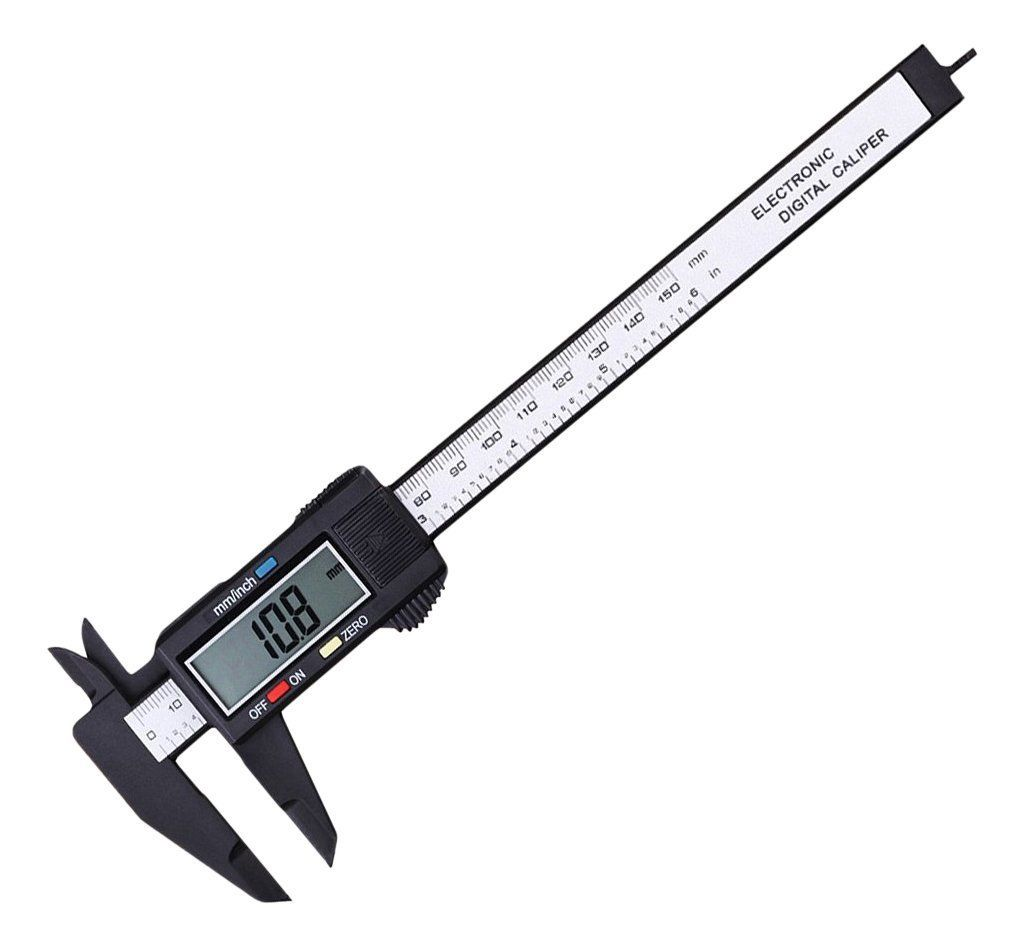
\includegraphics[width=\imas,valign=c]{images/digital_vernier_caliper.jpg} & Enables precise and accurate measurement of small dimensions, such as the width, thickness, and length of the alloys gauge, crucial for ensuring consistency in the data calculations for accurate results. \\
        Vickers Hardness Testing Machine & 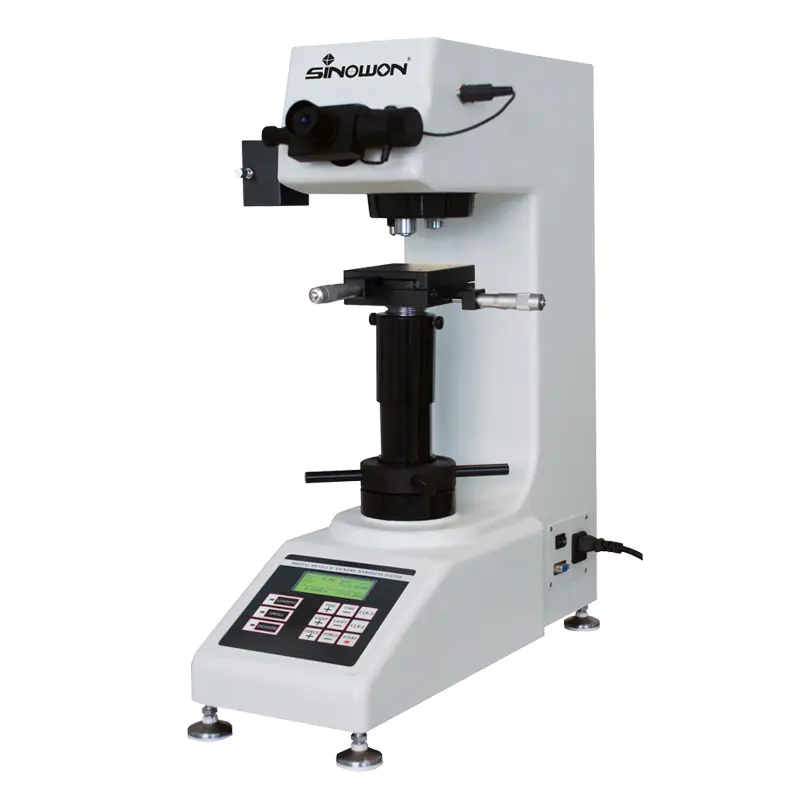
\includegraphics[width=2.1cm,height=2.4cm,valign=c]{images/hardness.png} & Used to measure the hardness of the alloys by applying a standardized force to create an indentation, which is then used to assess and determine the material's resistance to deformation. \\
        Zwick Roell 2050 Tensile Testing Machine & 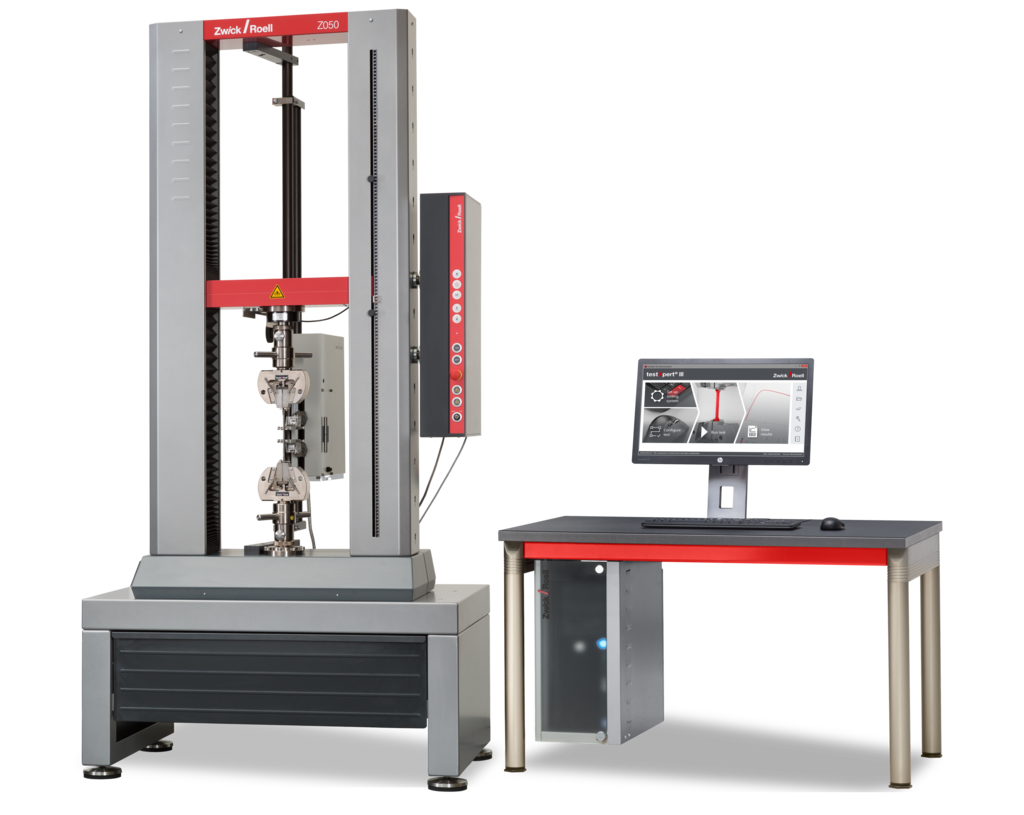
\includegraphics[width=\imas,valign=c]{images/tensilemachine.png} & Evaluates the tensile strength and mechanical properties of the alloys under uniaxial tension, providing data essential for material performance analysis and comparisons. \\
        \textbf{Personal Protective Equipment (PPE):} Safety glasses, closed-toe shoes, lab coat & 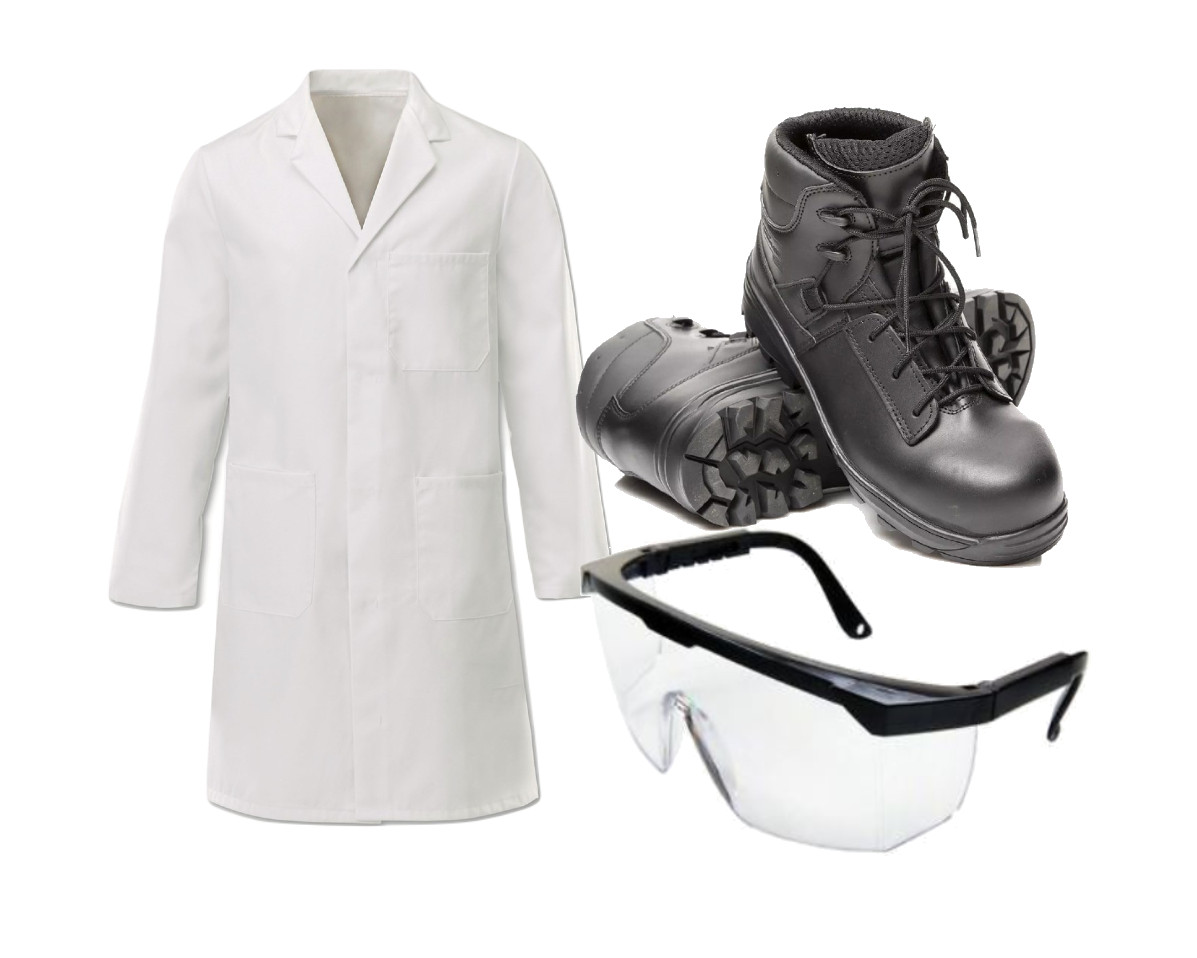
\includegraphics[width=\imas,valign=c]{images/ppe.jpg} & Protects against potential hazards in tensile testing, such as flying debris from specimen fracture, pinch points in the testing machine, and general laboratory risks further shown in Table \ref{tab:risk-assessment}.\\
        Camera/Smartphone and Stationery & 
\includegraphics[width=\imas,valign=c]{images/stationary.png} & For documenting experimental setups, procedures, capturing visual evidence of results, recording detailed observations, calculations, and procedural notes for accurate reporting. \\
    \end{tblr}
    \caption{Overview of Equipment Used in the Experiment}
    \label{tab:equipment_overview}
\end{table}

    

\newcommand{\mr}[2]{%
    \begin{varwidth}{#2}%
        #1%
    \end{varwidth}%
}


\subsection{Risk Assessment}
The experimental procedures involved several potential hazards. The identified risks, their levels, and mitigation strategies are outlined below:
\begin{table}[h!]
    \centering
    \begin{tblr}{
            width=\linewidth,
            colspec={Q[4cm]Q[5cm]Q[2cm,c,m]Q[5cm]},
            rows = {ht=4\baselineskip},
            row{1} = {font=\bfseries,c,m,ht=1.5\baselineskip},            
            rows,columns = {valign=m},
            hlines, vlines
        }
        Hazard & Risk & Level of Risk & Control Measures \\
        Tensile testing machine & \mr{Pinching or crushing injuries from moving parts}{5cm} & High & Keep hands and body away from moving components during operation; follow machine's safety protocols. \\
        \mr{Sharp edges of dogbone samples}{4cm} & \mr{Cuts or injuries while handling samples}{5cm} & Medium & \mr{Handle with care; use gloves when measuring and mounting samples.}{5cm} \\
        \mr{Vickers hardness testing machine}{4cm} & Injury from improper handling or sample misplacement & Medium & Ensure proper training before operation; position samples correctly and keep fingers clear. \\
        \mr{General laboratory environment}{4cm} & Slips, trips, and falls due to clutter or spills & Low & Maintain a tidy workspace; clean spills immediately; wear appropriate footwear. \\
    \end{tblr}
    \caption{Identified hazards, associated risks, levels, and control measures.}
    \label{tab:risk-assessment}
\end{table}

\section{Conducting the Experiment}
For the experiment, we were provided with three samples, which are visually represented in the image below:
\begin{figure}[H] 
    \centering 
    \includegraphics[width=0.6\textwidth,height=0.3\textheight]{example-image} 
    \caption{Visual representation of the three samples} 
    \label{fig:samples} 
\end{figure}
\newpage\noindent
Additionally, we were given an A4 sheet with a form to complete, as shown below:

\begin{figure}[H] 
    \centering 
    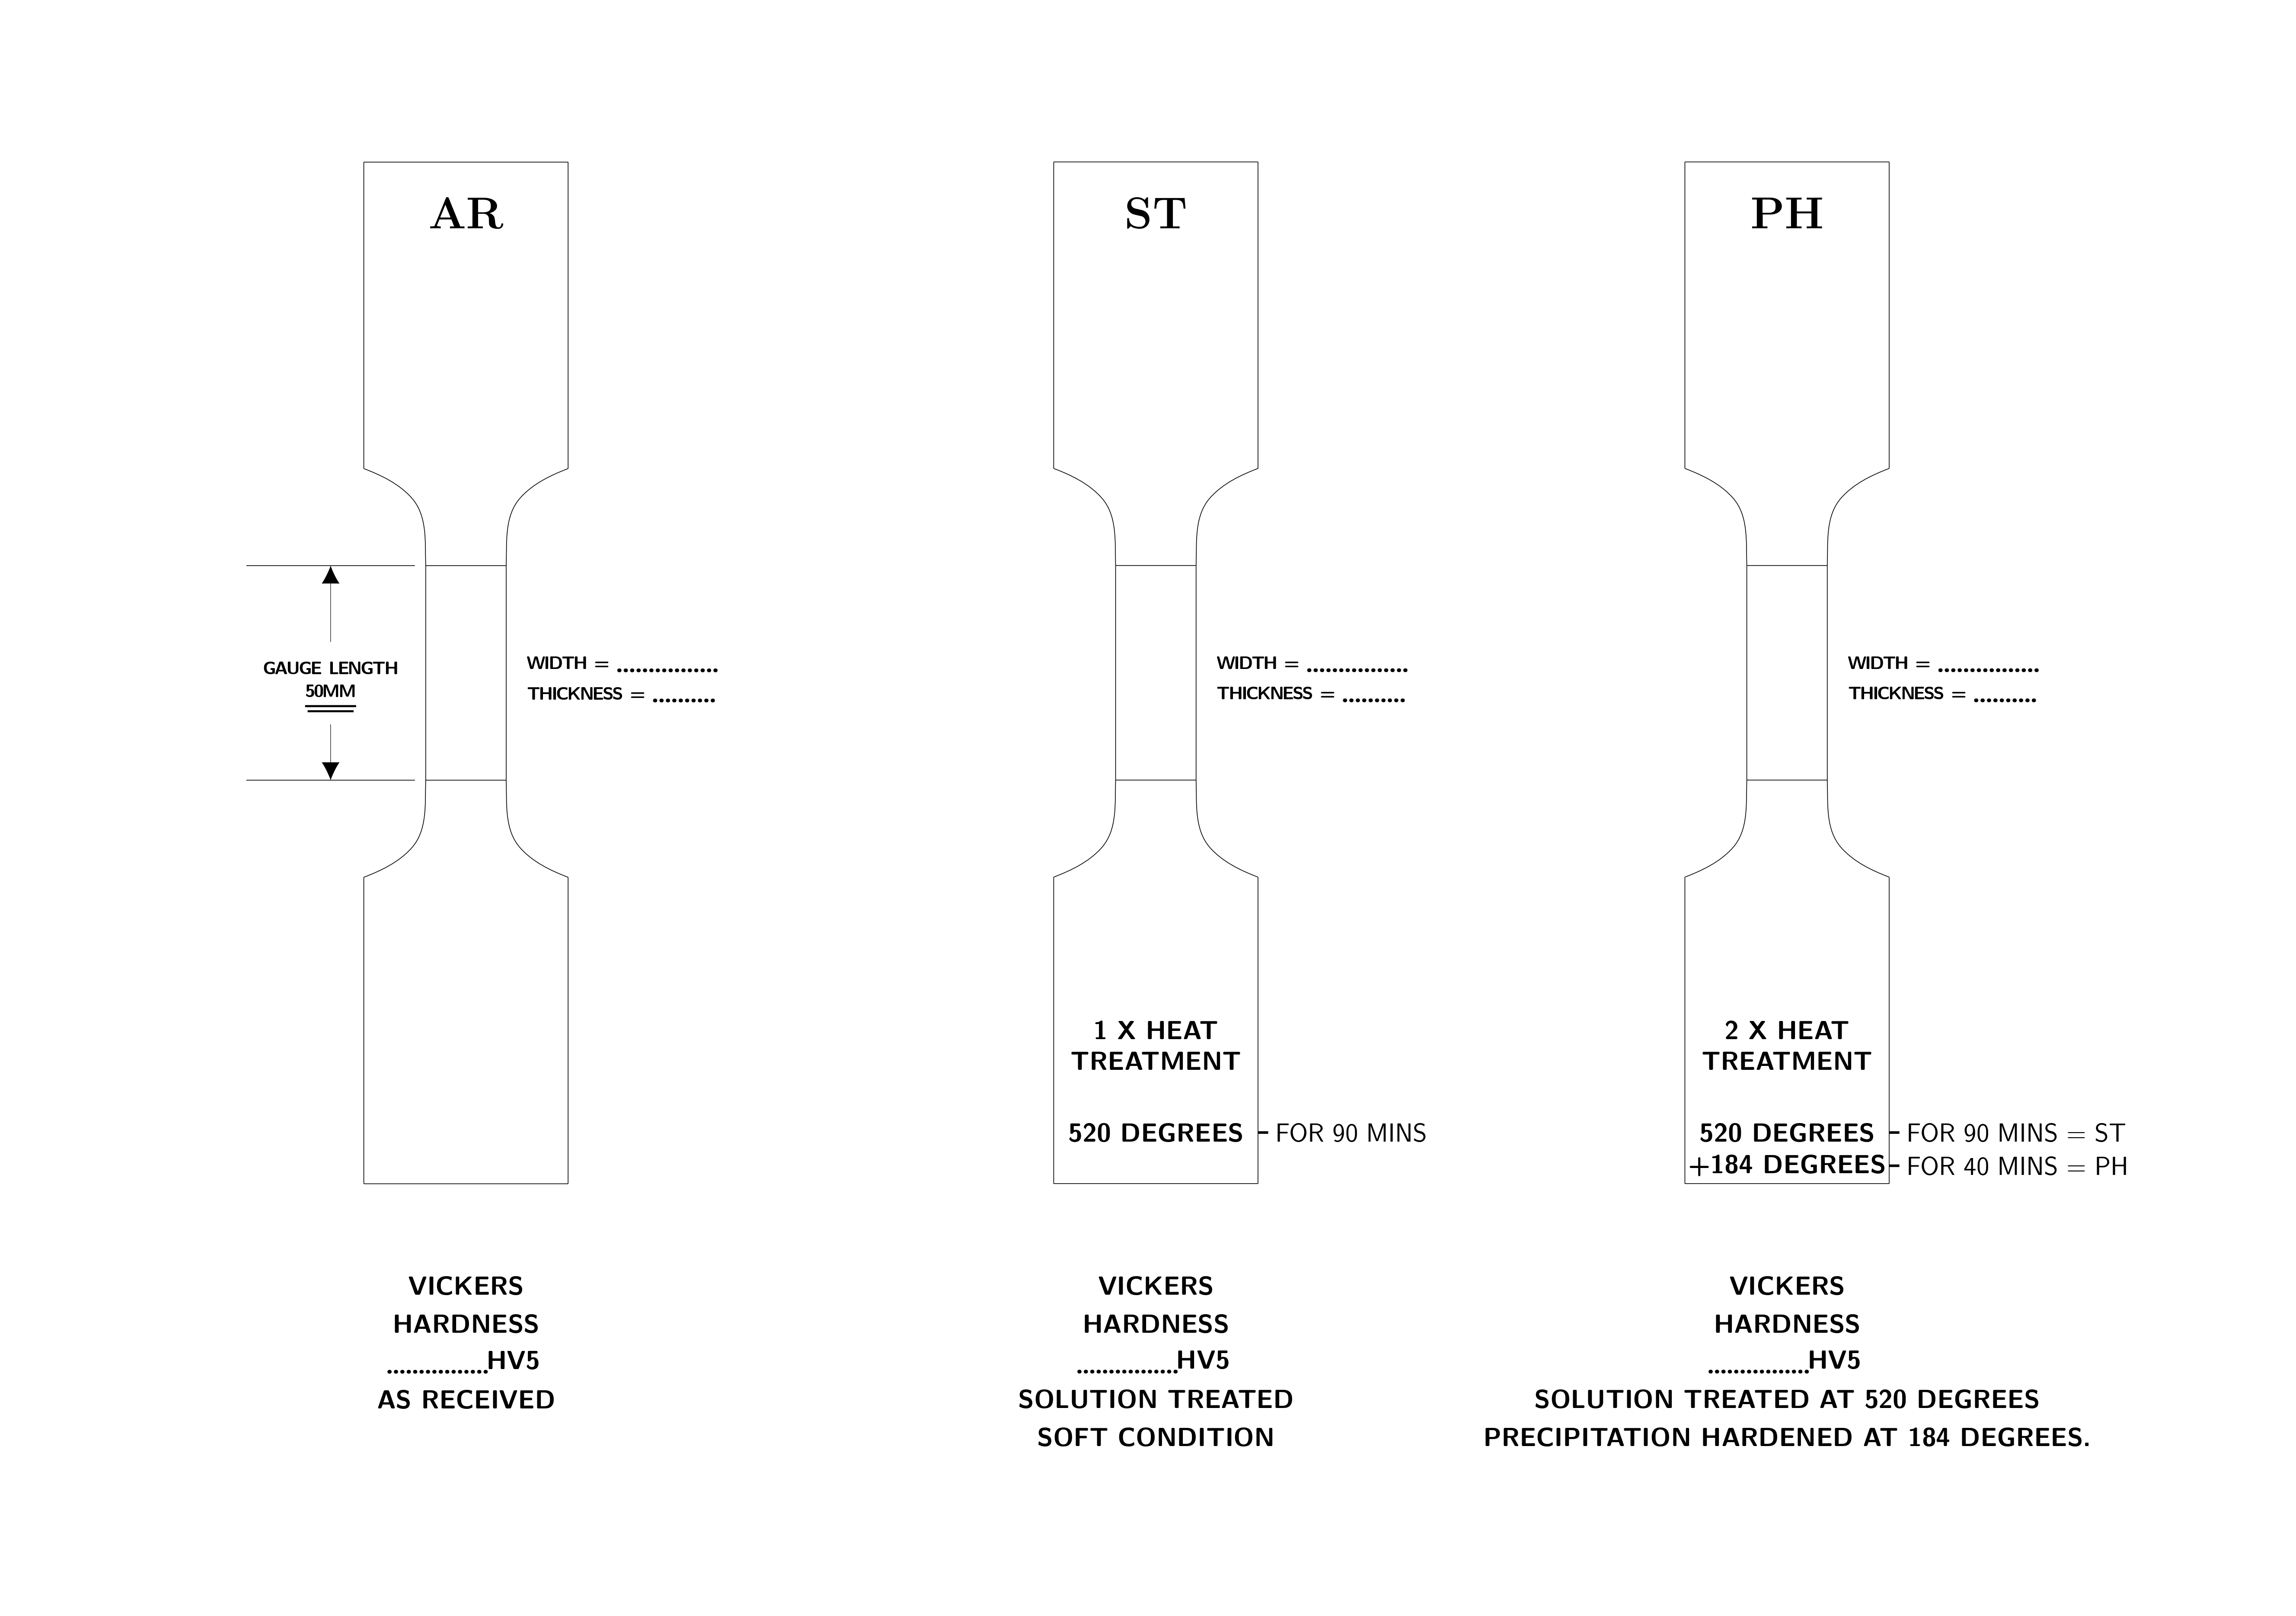
\includegraphics[width=0.95\textwidth,cfbox=gray!22 1pt]{figures/alloys_base.jpg} % LoL this shit would have been like 1k plus line at the least
    \caption{Form for recording sample measurements and hardness} 
    \label{fig:alloys} 
\end{figure}

\textbf{General Overview:}
The experiment was conducted in two phases: measuring the dimensions and hardness of alloy samples, followed by testing their tensile properties with the Zwick Roell 2050 Tensile Testing Machine. \\[8pt]
In the first phase, the width and length of each sample were recorded using digital calipers (in millimeters), while hardness was measured with a Vickers Hardness test machine using the HV5 scale. These tasks were conducted simultaneously, as both are quick and independent processes.\\[8pt]
After documenting the dimensions and hardness on the data sheet (See Figure \ref{fig:alloys}), we proceeded to the second phase of the experiment, were each sample was subjected to a controlled tensile force until fracture using the Zwick Roell 2050 Tensile Testing Machine. The data, including force applied vs change in length was recorded on a shared graph for all three alloys, this along with a table outlining key metrics for the respective graphs.\\[8pt] 
This information was printed on an A4 sheet and given for additional examination outside of the lab (see Figure \ref{fig:tensile_results}). Important parameters, including stress, strain, yield strength, uts, and others are to be calculated after the experiment and are presented as a key part of analysis in this report.\\[8pt]
The following subsections detail the use of the equipment, outlining each step of the procedure.\\
\newpage\newgeometry{margin=1in,right=0.8in,left=0.8in,bottom=0.65in}
\begin{minipage}{0.32\textwidth}
\hspace{2em}
\begin{tikzpicture}[rotate around y=225, use Hobby shortcut,scale=0.35, every node/.style={scale=0.35}]
    \LARGE
    \def\width{4}
    \def\gap{10}
    \def\main{8}
    \def\curvy{1.9}
    \def\depth{3}
    
    \def\n{3.3}
    \def\z{1/\n}
    \pgfmathsetmacro{\s}{1-\z}
    
    \coordinate (A) at (0,\main,0);
    \coordinate (B) at (\width*\z-\width*\z*0.23,\main+\curvy-\curvy*0.7,0);
    \coordinate (C) at (\width*\z,\main+\curvy,0);
    
    \coordinate (A2) at (\width,\main,0);
    \coordinate (B2) at (\width*\s+\width*\z*0.23,\main+\curvy-\curvy*0.7,0);
    \coordinate (C2) at (\width*\s,\main+\curvy,0);
    
    \coordinate (A3) at (0,\main+\gap,0);
    \coordinate (B3) at (\width*\z-\width*\z*0.23,\main+\gap-\curvy+\curvy*0.7,0);
    \coordinate (C3) at (\width*\z,\main+\gap-\curvy,0);
    
    \coordinate (A4) at (\width,\main+\gap,0);
    \coordinate (B4) at (\width*\s+\width*\z*0.23,\main+\gap-\curvy+\curvy*0.7,0);
    \coordinate (C4) at (\width*\s,\main+\gap-\curvy,0);
    
    % Back variation with \depth (subtracting \depth from the z-coordinate)
    \coordinate (A') at (0,\main,\depth);
    \coordinate (B') at (\width*\z-\width*\z*0.23,\main+\curvy-\curvy*0.7,\depth);
    \coordinate (C') at (\width*\z,\main+\curvy,\depth);
    
    \coordinate (A2') at (\width,\main,\depth);
    \coordinate (B2') at (\width*\s+\width*\z*0.23,\main+\curvy-\curvy*0.7,\depth);
    \coordinate (C2') at (\width*\s,\main+\curvy,\depth);
    
    \coordinate (A3') at (0,\main+\gap,\depth);
    \coordinate (B3') at (\width*\z-\width*\z*0.23,\main+\gap-\curvy+\curvy*0.7,\depth);
    \coordinate (C3') at (\width*\z,\main+\gap-\curvy,\depth);
    
    \coordinate (A4') at (\width,\main+\gap,\depth);
    \coordinate (B4') at (\width*\s+\width*\z*0.23,\main+\gap-\curvy+\curvy*0.7,\depth);
    \coordinate (C4') at (\width*\s,\main+\gap-\curvy,\depth);
    
    
    % Back face fill
    \fill[black!40] 
    (0,0,\depth) -- (\width,0,\depth) -- (\width,\main,\depth) 
    to[hobby,tension=3] (\width,\main,\depth) .. (\width*\s+\width*\z*0.23,\main+\curvy-\curvy*0.7,\depth) .. (\width*\s,\main+\curvy,\depth) -- 
    (\width*\s,\main+\gap-\curvy,\depth) 
    to[hobby,tension=3] (\width*\s,\main+\gap-\curvy,\depth)  .. (\width*\s+\width*\z*0.23,\main+\gap-\curvy+\curvy*0.7,\depth) .. (\width,\main+\gap,\depth) --
    (\width,2*\main+\gap,\depth) -- (0,2*\main+\gap,\depth) -- 
    (0,\main+\gap,\depth) to[hobby,tension=3] (0,\main+\gap,\depth) .. (\width*\z-\width*\z*0.23,\main+\gap-\curvy+\curvy*0.7,\depth) .. (\width*\z,\main+\gap-\curvy,\depth) --
    (\width*\z,\main+\curvy,\depth) to[hobby,tension=3] (\width*\z,\main+\curvy,\depth) .. (\width*\z-\width*\z*0.23,\main+\curvy-\curvy*0.7,\depth) .. (0,\main,\depth) --
    cycle;
    
    % Curves fills with refined fades
    \fill[left color=gray!80, middle color=gray!50, right color=gray!20, opacity=0.8] 
    (A) to[hobby,tension=3] (A) .. (B) .. (C) -- (C3) to[hobby,tension=3] (C3) .. (B3) .. (A3) -- 
    (A3') to[hobby,tension=3] (A3') .. (B3') .. (C3') --
    (C') to[hobby,tension=3] (C') .. (B') .. (A') -- cycle;
    
    \fill[left color=gray!80, middle color=gray!50, right color=gray!20, opacity=0.8] 
    (A2) to[hobby,tension=3] (A2) .. (B2) .. (C2) -- (C4) to[hobby,tension=3] (C4) .. (B4) .. (A4) -- 
    (A4') to[hobby,tension=3] (A4') .. (B4') .. (C4') --
    (C2') to[hobby,tension=3] (C2') .. (B2') .. (A2') -- cycle;
    
    
    \draw[-,hobby,tension=3] (A2') .. (B2') .. (C2');
    \draw[-,hobby,tension=3] (A4') .. (B4') .. (C4');
    
    % Fill for bottom rectangle section
    \fill[black!33] 
    (0,0,0) -- (\width,0,0) -- (\width,0,\depth) -- (0,0,\depth) -- cycle;
    \fill[black!33] 
    (0,0,0) -- (0,\main,0) -- (0,\main,\depth) -- (0,0,\depth) -- cycle;
    \fill[black!40] 
    (\width,0,0) -- (\width,\main,0) -- (\width,\main,\depth) -- (\width,0,\depth) -- cycle;
    
    % Fill for top rectangle section
    \fill[black!30] 
    (0,2*\main+\gap,0) -- (\width,2*\main+\gap,0) -- (\width,2*\main+\gap,\depth) -- (0,2*\main+\gap,\depth) -- cycle;
    \fill[black!30] 
    (0,\main+\gap,0) -- (0,2*\main+\gap,0) -- (0,2*\main+\gap,\depth) -- (0,\main+\gap,\depth) -- cycle;
    \fill[black!33] 
    (\width,\main+\gap,0) -- (\width,2*\main+\gap,0) -- (\width,2*\main+\gap,\depth) -- (\width,\main+\gap,\depth) -- cycle;
    
    
    
    % Front face fill
    \fill[black!36] 
    (0,0,0) -- (\width,0,0) -- (\width,\main,0) 
    to[hobby,tension=3] (A2) .. (B2) .. (C2) -- 
    (\width*\s,\main+\gap-\curvy,0) 
    to[hobby,tension=3] (C4) .. (B4) .. (A4) --
    (\width,2*\main+\gap,0) -- (0,2*\main+\gap,0) -- 
    (0,\main+\gap,0) to[hobby,tension=3] (A3) .. (B3) .. (C3) --
    (\width*\z,\main+\curvy,0) to[hobby,tension=3] (C) .. (B) .. (A) --
    cycle;
    \draw[hobby,tension=3] (A) .. (B) .. (C);
    \draw[hobby,tension=3] (A2) .. (B2) .. (C2);
    \draw[hobby,tension=3] (A3) .. (B3) .. (C3);
    \draw[hobby,tension=3] (A4) .. (B4) .. (C4);
    \draw[dashed, opacity=0.3,hobby,tension=3] (A3') .. (B3') .. (C3');
    \draw[dashed, opacity=0.3,hobby,tension=3] (A') .. (B') .. (C');
    % Front face outline
    
    \draw[-] (0,0,0) -- (\width,0,0);
    \draw[-] (0,0,0) -- (0,\main,0);
    \draw[-] (\width*\z,\main+\curvy,0) -- (\width*\z,\main+\gap-\curvy,0);
    \draw[-] (0,\main+\gap,0) -- (0,2*\main+\gap,0);
    \draw[-] (0,2*\main+\gap,0) -- (\width,2*\main+\gap,0);
    \draw[-] (\width,2*\main+\gap,0) -- (\width,\main+\gap,0);
    \draw[-] (\width*\s,\main+\curvy,0) -- (\width*\s,\main+\gap-\curvy,0);    
    \draw[-] (\width,0,0) -- (\width,\main,0);
    
    
    
    
    
    % Back face outline
    
    
    \draw[dashed, opacity=0.3] (\width*\z,\main+\curvy,\depth) -- (\width*\z,\main+\gap-\curvy,\depth);
    \draw[-] (\width*\s,\main+\curvy,\depth) -- (\width*\s,\main+\gap-\curvy,\depth);
    \draw[dashed, opacity=0.3] (0,0,\depth) -- (\width,0,\depth);
    \draw[dashed, opacity=0.3] (0,0,\depth) -- (0,\main,\depth);
    \draw[-] (\width,0,\depth) -- (\width,\main,\depth);
    \draw[dashed, opacity=0.3] (0,\main+\gap,\depth) -- (0,2*\main+\gap,\depth);
    \draw[-] (0,2*\main+\gap,\depth) -- (\width,2*\main+\gap,\depth);
    \draw[-] (\width,2*\main+\gap,\depth) -- (\width,\main+\gap,\depth);
    
    
    
    % Connect front and back faces
    %botom
    \draw[-] (\width,\main,0) -- (\width,\main,\depth);
    \draw[-] (\width,0,0) -- (\width,0,\depth);
    \draw[dashed, opacity=0.3] (0,0,0) -- (0,0,\depth);
    \draw[-] (0,\main,0) -- (0,\main,\depth);
    %top
    \draw[-] (\width,\main+\gap,0) -- (\width,\main+\gap,\depth);
    \draw[-] (\width,2*\main+\gap,0) -- (\width,2*\main+\gap,\depth);
    \draw[-] (0,2*\main+\gap,0) -- (0,2*\main+\gap,\depth);
    \draw[dashed, opacity=0.3] (0,\main+\gap,0) -- (0,\main+\gap,\depth);
    
    
    
    %curves
    
    \draw[{Latex[length=1.93mm,width=1.93mm]}-{Latex[length=1.93mm,width=1.93mm]},line width=0.5mm] (C) -- (C2) node[below=-3,right=45] {\Huge \textbf{Width}};
    \draw[dashed, opacity=0.3] (C3) -- (C4);
    \draw[dashed, opacity=0.3] (C') -- (C2');
    \draw[dashed, opacity=0.3] (C3') -- (C4');
    \draw[dashed, opacity=0.3] (C) -- (C');
    \draw[{Latex[length=1.93mm,width=1.93mm]}-{Latex[length=1.93mm,width=1.93mm]},line width=0.5mm] (C2) -- (C2') node[below=-2,left] {\Huge \textbf{Thickness}};
    \draw[dashed, opacity=0.3] (C3) -- (C3');
    \draw[dashed, opacity=0.3] (C4) -- (C4');
    
    \draw[latex-latex, line width=0.5mm] 
    ($ (C) - (0.4,0,0) $) 
    -- ($ (C3) - (0.4,0,0) $) 
    node[right=5, midway] {\Huge \textbf{Length}};
    
\end{tikzpicture}
\end{minipage}\hfill
\begin{minipage}{0.65\textwidth}
\subsection{Measurements}\label{Measurements}
\vspace{0.5em}
\begin{center}
    \begin{tblr}{
        width=\textwidth,
        colspec={X[2,c]X[1,c]X[1,c]X[1,c]},
        hlines,vlines,
        rows={ht=1\baselineskip},
        row{1} = {ht=1\baselineskip,font=\bfseries,c,m},
        cells={valign=m,halign=c}
    }
    Property (mm) & AR & ST & PH \\
    Width   & 11.98 & 12.00 & 11.97 \\
    Thickness & 6.00  & 6.38  & 6.18  \\
    Length & 50.00 & 50.00 & 50.00 \\
\end{tblr}
\end{center}
\captionof{table}{Dimensions of AR, ST, and PH}
\label{tab:dimensions}
\vspace{1em}
\noindent
We measured the dimensions of each alloys gauge region using a digital calliper and recorded the results on the data sheet (See Figure \ref{fig:alloys}). We were informed that the gauge length was 50 mm, but we did not measure it ourselves.\\[8pt] 
Although checking measurements is good practice, it was determined the cross-sectional area (CSA) analysis does not require it, \textbf{however} it is needed for further analysis for several other parameters in the data section.
\end{minipage}
\subsection{Hardness Test}
To evaluate the hardness of our alloys, we employed the Vickers Hardness (HV) test, among others methods (See Section \ref{hardnesstypes}).\\[8pt]
The Vickers Hardness (HV) test is known as a precise and versatile method for measuring material hardness through indentation. It employs a diamond-shaped indenter with a square base at an included angle of 136\textdegree \ between opposing faces (See Figure \ref{fig:vickers-diagram}) (Ultramag, 2024; ZwickRoell, 2024).\\[8pt]
\begin{minipage}{0.55\textwidth}
    The indenter is pressed into the material under a specific load, typically ranging from 1 to 100 kgf\footnotemark, applied for 10 to 15 seconds (Ultramag, 2024). In our case, a load of 5 kgf (approximately \SI{49.03}{\newton}) was applied for a duration of approximately 1–5 seconds. This test is referred to as HV5.\\[8pt]
    The process began by pressing the indenter onto the alloy surface, creating an indent.\\[8pt] 
    Afterward, using a dial, we adjusted the two parallel lines to align with the indent, measuring the first distance, \(d_1\), ensuring the indent was accurately positioned between the two sides (See Figure \ref{fig:vickers}).\\[8pt]
    Once the first measurement was confirmed, we repositioned the sample and took the second distance measurement, \(d_2\), for the indent.
\end{minipage}\hspace{1em}
\begin{minipage}{0.4\textwidth}\centering
\begin{figure}[H]
    \centering
    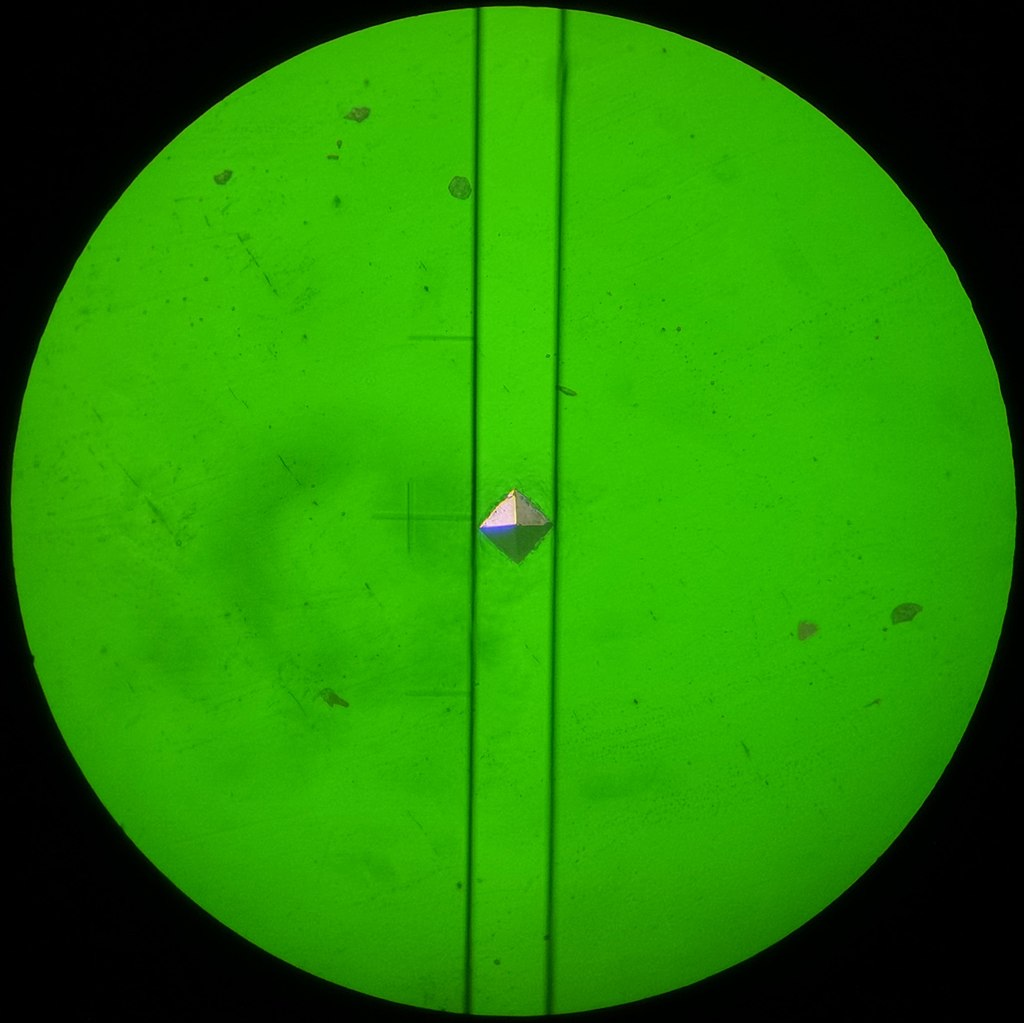
\includegraphics[width=0.8\textwidth]{images/1024px-Vicker_Hardness_-_Diamond_Indentation.jpg}
    \caption{Illustration showing the indent and the parallel lines used for measuring the indentation. (Wikipedia)}
    \label{fig:vickers}
\end{figure}
\end{minipage}\\[8pt]\footnotetext{{1 kilogram-force (kgf) is the force exerted by one kilogram of mass under standard gravity (\SI{9.81}{\meter\per\second\squared}), approximately equal to \SI{9.81}{\newton}.}}Finally, once both distances were recorded by the machine, we pressed a button to calculate the hardness.
\newpage\newgeometry{left=0.8in,right=0.8in,bottom=0.9in}
To ensure accuracy and consistency, this process was done at least 2-3 times for each given alloy and the resulting hardness values were recorded on the data sheet (See Figure \ref{fig:alloys}) for later analysis.\\[8pt]
Although the machine automatically calculates the hardness, it is important to understand the underlying process. The Vickers hardness is determined by a fixed force and the indentation area, which is calculated using the average of the diagonals $d_1$ and $d_2$, along with the indentation geometry (ZwickRoell, 2024). I demonstrate and derive the pertinent equation and calculation for the HV5 test within theory section (See Section \ref{meanhard}).\\[8pt]
The recorded results were documented on the data sheet as follows:\\
\vspace{0.3em}
\begin{center}
    \begin{tblr}{
            width=\textwidth,
            colspec={X[3,c]X[0.75,c]X[0.75,c]X[0.75,c]X[0.75,c]X[0.75,c]X[0.75,c]X[0.8,c]X[0.8,c]X[0.8,c]},
            hlines,vlines,
            rows={ht=1\baselineskip},
            row{1} = {ht=1\baselineskip,font=\bfseries,c,m},
            cells={valign=m,halign=c}
        }
        Property (\(\bm{\text{unitless}}\)) & \SetCell[c=2]{c} AR & & \SetCell[c=2]{c} ST & & \SetCell[c=3]{c} PH & & \\
        HV5 (Individual) & 119 & 123 & 36 & 36.8 & 102.8 & 131 & 126 \\
    \end{tblr}
    \captionof{table}{HV5 Data}
    \label{tab:hv5}
\end{center}
\vspace{0.3em}
Here Table \ref{tab:hv5} shows the individual Vickers hardness (HV5) values for each alloy, with averages to be calculated in the Data and Results section.\\[8pt]
\vspace{1em}
\begin{minipage}{0.4\textwidth}
    \begin{figure}[H]
    \centering
    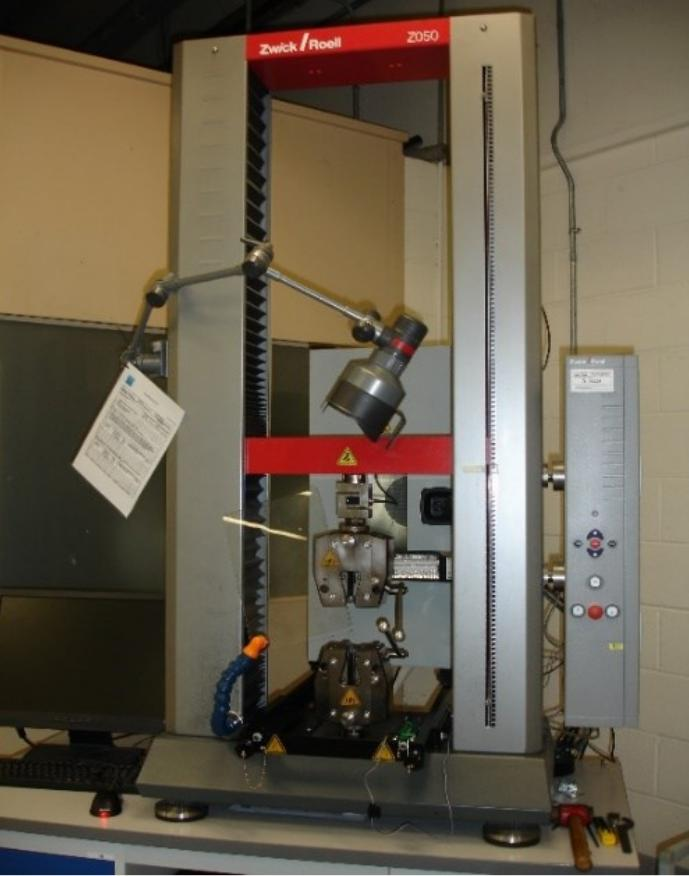
\includegraphics[width=0.8\textwidth]{images/tensile_machine.jpg}
    \caption{A Zwick tensile 50 kN testing similar to the one used}
    \label{fig:tensile_machine}
    \end{figure}
\end{minipage}\hfill
\begin{minipage}{0.555\textwidth}
\subsection{Tensile Test}
This phase of the experiment focused tensile testing to assess the alloy's mechanical characteristics. The tensile tester used in this lab was a {Zwick machine}, with a maximum load capacity of 50 kN and an adjustable pulling rate (See Figure \ref{fig:tensile_machine}).\\[8pt]
An axial load was applied to the standardised dog-bone-shaped alloy as part of the destructive test procedure. The alloy, which had a precisely sized gauge length, was held firmly at both ends and extended at a regulated pace until it broke.\\[8pt]
For analysis, a real-time plot of force (N) versus change in length (mm) was generated during the experiment.
\end{minipage}\\[8pt]
Once the test was completed, i.e., after the specimen broke, the system also provided a table outlining details such as \textbf{Maximum Load (N)} \& \textbf{Extension at Break (mm)} \footnote{Table title terminology has been reworded for clarity. The original table titles are phrased strangely and incorrectly in a sense. A more detailed explanation and possible justification is provided in a later section.}. This process was automated using the manufacturer's software. The machine did not account for the sample's thickness or width, or simply by observation it was not given, making the data for these parameters invalid.\\[8pt]
To gain further insights, we must relate the generated data to the initial measurements (e.g., cross-sectional area and gauge length (see Section \ref{Measurements})). Although inputting these values directly into the machine could have provided more prevalent tables and stress-strain curves, this was likely avoided to promote independent analysis and a deeper understanding of the process.

\begin{figure}[H]
    \centering    
    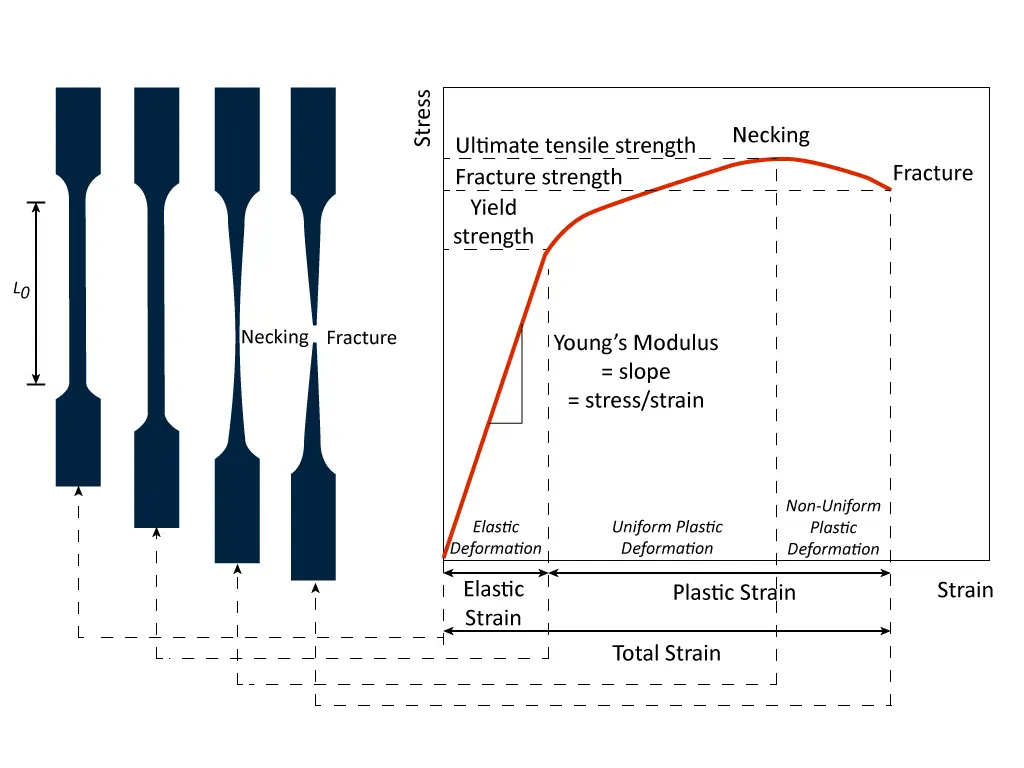
\includegraphics[width=0.7\textwidth]{images/simwiki-stress-strain-shape-evolution.png}
    \captionof{figure}{The shape of a ductile specimen changes during tensile testing (ADMET, 2017)}
    \label{fig:alloys_next_graph}
\end{figure}
This stress-strain graph, though not produced during our lab, illustrates key regions corresponding to visual changes in the alloy. While our real-time force vs. change in length graph isn't a true stress-strain curve, it represents similar principles due to proportional relationships. Thus, observed deformations can be linked to these stages. (For Further explanations see Section \ref{tt}).\\[8pt]
The procedure followed during the tensile test was as follows: 
\begin{enumerate}
    \item We ensured all safety precautions, including wearing safety glasses and maintaining a safe distance (approximately 1.5 meters) from the equipment before starting the test.
    \item Upon initiating the test by clicking the "Start" button, the upper and lower grips moved in opposite directions according to the set pulling rate.
    \item The initial \textbf{elastic deformation region}, where the material experienced reversible stretching, was not noticeably perceptible in the alloys if not closely observant, due to the small change in length during this phase.\footnote{This region also corresponds to the Lüders region, where some materials undergo localized yielding before uniform plastic deformation. Whether this occurred in our alloy is uncertain, as I do not observe it in the graph produced by the machine (see Figure \ref{fig:tensile_results}). Regardless, no visible change in the material's shape or bands is seen during this phase.}
    \item Following the elastic region, the material enters the \textbf{uniform plastic deformation region}, where the material elongates uniformly across the specimen, and the elongation becomes more noticeable, with no localized necking occurring as of yet.
    \item The first noticeable event was \textbf{necking}, which appears as a localized narrowing of the material in the gauge length area, signaling the beginning of plastic deformation. This is the point where the material begins to stretch unevenly.
\end{enumerate}
\newpage
\begin{enumerate}
    \item[6.] After necking, in the \textbf{non-uniform plastic deformation region}, the graph displayed distinct behaviors (though the earlier regions also exhibited varying characteristics in the rate of change) depending on the alloy being tested (see Figure \ref{fig:stress_strain}):
    \begin{itemize}
        \item For the solution-treated (ST) alloy, necking continued to propagate slowly, allowing further elongation before breaking, with the neck widening visibly before final failure.
        \item For the as-received (AR) and precipitation-hardened (PH) alloys, necking intensified rapidly, resulting in a more pronounced narrowing of the specimen and leading to quicker fracture.
    \end{itemize}
    The plot produced captured these differences, showing a sharp drop in force once the material reached its breaking point (See Figure \ref{fig:force_elong}).
\end{enumerate}
Once all three alloys broke, we were left with a shared force vs. change in length data and a table of results from the machine for all three alloys, this was to be printed all on an A4 sheet by ZwickRoell.\\ 
\vspace{3em}
\begin{center}
    \begin{minipage}{0.45\textwidth}
    \centering    
    \includegraphics[width=\textwidth]{images/image(6).jpeg}
    \captionof{figure}{The three broken alloys, showing the final stage of deformation after tensile testing.}
    \label{fig:broken_alloys}
\end{minipage}%
\hfil
\begin{minipage}{0.45\textwidth}
    \centering    
    \includegraphics[width=\textwidth]{example-image}
    \captionof{figure}{A4 machine data, including shared table and graph of alloys.}
    \label{fig:tensile_results}
     \footnotemark 
\end{minipage}
\end{center}
    \footnotetext{This is better represented in the Data and Result section}

   \newpage

    \section{Theory}
    
    In this section, I will outline the theoretical foundations underlying the methods and analyses used in this experiment. This includes the conceptual frameworks, mathematical models, and principles that explain the phenomena under investigation.\\[8pt]
    By detailing the reasoning behind the techniques and approaches employed, I aim to establish a solid foundation for the experimental procedures and data analysis, ensuring that the conclusions drawn are based on sound scientific principles.\\[8pt]
    Important theoretical ideas pertaining to our lab's work will be covered in this part, namely:
    \begin{itemize}
        \item \textbf{Hardness}
        \item \textbf{Tensile Testing}
        \begin{itemize}
            \item \textbf{Stress \& Strain}
            \item \textbf{Young's Modulus}
            \item \textbf{Hooke's Law}
            \item \textbf{Yield Point}
            \item \textbf{Modulus of Resilience}
            \item \textbf{Ultimate Tensile Strength (UTS)}
            \item \textbf{Modulus of Toughness}
            \item \textbf{Ductility}
            \item \textbf{Material Property Ratios}
        \end{itemize}
    \end{itemize}
    Understanding all these properties will enable us to fully characterize the mechanical performance of the material under stress, allowing us to calculate them from the data collected during the experiment and fully assess our alloy.
    \newpage
   \subsection{Hardness}\label{hardnesstypes}
    Hardness is a material property that measures its resistance to deformation, scratching, or penetration by external forces. It is a critical factor in evaluating the durability and wear resistance of materials, often used in material science and engineering to determine suitability for specific applications (ScienceDirect, n.d.).\\[8pt]
    The concept of hardness is multifaceted, encompassing several types:
    \begin{itemize}
        \item \textbf{Scratch Hardness}: The resistance of a material to scratching, often assessed using the Mohs scale, which ranks materials based on their ability to scratch one another.
        \item \textbf{Indentation Hardness}: This measures resistance to permanent deformation under localized pressure, typically using methods like the Brinell, Vickers, Rockwell or Knoop hardness tests.
        \item \textbf{Rebound Hardness}: The ability of a material to resist impact, evaluated through methods such as the Shore scleroscope test.
    \end{itemize}
    These approaches rely on different theoretical principles. For instance, indentation hardness tests use mathematical models to relate the force applied and the resulting deformation, often involving elastic and plastic deformation mechanics. The Mohs scale, on the other hand, is more qualitative and based on empirical observations.\\[8pt]
    Understanding hardness is essential in applications ranging from manufacturing to material selection, where wear resistance, strength, and surface durability are critical considerations.\\[1.5em]

    \begin{figure}[H]
        \centering
        \begin{minipage}{0.45\textwidth}
            \vspace{-1em}
            \subsubsection{Vickers Hardness Calculation}\label{VHC}
            
            \centering
            \vspace{2em}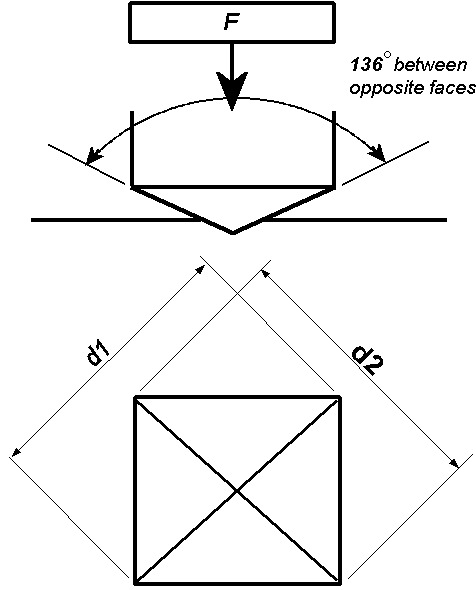
\includegraphics[width=0.8\textwidth]{figures/3537580_orig-0000.jpg}
            \caption{Diagram showing the diamond-shaped indenter with the 136° angle and diagonals \(d_1\) and \(d_2\). (ResearchGate, 2009)}
            \label{fig:vickers-diagram}
        \end{minipage}\hfill
        \begin{minipage}{0.51\textwidth}
            The Vickers hardness (HV) is calculated using the applied force (\(F\)) and the surface area (\(A\)) of the indentation. 
            \begin{equation}
                \text{HV} = \frac{F}{A}
            \end{equation}
            Where:
            \begin{itemize}[itemsep=-1mm]
                \item HV: Vickers hardness (dimensionless)
                \item \(F\): Applied force (kilogram-force, \(\text{kgf}\)) or (Newtons, \(\text{N}\))
                \wm{\item \(A\): Surface area of the indentation (millimetres \\squared, \(\text{mm}^2\))}            
            \end{itemize}
            The formula for $A$ incorporates the geometry of the diamond pyramid indenter, such that surface area \(A\) can be expressed as:
            \begin{equation}
                A = \frac{d^2}{2\sin\left(\frac{136^\circ}{2}\right)} \approx \frac{d^2}{1.854} 
            \end{equation}
            \begin{itemize}[itemsep=-1mm]
                \item \( d \): Arithmetic mean of the diagonals \( d_1 \) and \( d_2 \) (millimetres, \(\text{mm}\))
            \end{itemize}
            so that it can be expressed in terms of the diagonals as follows:
            \begin{equation}
                A= \frac{\left(\frac{d_1+d_2}{2}\right)^2}{2\sin\left(\frac{136^\circ}{2}\right)} \approx \frac{\left(d_1 + d_2\right)^2}{7.236}
            \end{equation}
        \end{minipage}\\
    \end{figure}
    \vspace{-1em}\newpage\noindent
    Thus the derived formula is commonly shown as
    \begin{equation}
        {\text{HV} = \frac{F}{A} \approx \, \frac{1.854 \times F}{d^2} \approx \, \frac{7.236\times F}{\left(d_1 + d_2\right)^2}}    
    \end{equation} 
    The HV5 test we conducted applied a fixed load of 5 kgf (49.03 N), and the hardness was calculated via the machine as:  
    \begin{equation}
        \text{HV5} = \frac{49.03}{A} \approx \, \frac{90.902}{d^2} \approx \, \frac{354.781}{\left(d_1 + d_2\right)^2}
    \end{equation}
    Values for \(d_1\) and \(d_2\) were obtained from the machine dial, and the corresponding hardness values were calculated accordingly. It is worth noting, if not already disclosed, that the resulting HV and HV5 values are expressed as dimensionless numbers. Special thanks to N.A.S.R.U.L DESIGN (2024) for their valuable insights and assistance with the logical framework.\\[1em]
    \hrule\vspace{1em}
    Going into detail about each type of hardness, along with their specific equations and characteristics, seems excessive for this context. I concentrated on Vickers hardness because it directly relates to the test we performed. My goal is to include only the information that is specifically relevant to this report.
    
    \newpage

    \subsection{Tensile Testing}\label{tt}
    
    \begin{formal}[iqytechnicalcollege, 2012]
        Tensile testing is used to establish operational load limits for metals and alloys. A sample of the material is prepared so that a force can be applied along its axis. A central portion of the sample is reduced in width so that it will experience the highest stresses.\\[8pt]
        The tensile test measures the ability of a material to support a stress (force per unit area). The response of a tensile sample to the application of an increasing stress can be described in terms of elastic and plastic behavior. Initially, the sample undergoes elastic elongation as it is pulled. As increasing stress is applied, the sample undergoes permanent deformation; that is, plastic strain.\\[8pt]
        A stress-strain curve is used to determine the point at which the reversible elastic strain is exceeded and permanent or plastic deformation occurs. The yield strength is the stress necessary to cause significant plastic deformation (usually defined as 0.2\% strain).\\[8pt]
        Young’s modulus, or the modulus of elasticity, states the relationship between stress and strain represented by the straight-line portion of the stress-strain curve. It reflects the tendency of a material to deflect under a given applied stress.\\[8pt]
        Once yielding has begun, there is significant motion of dislocations within the metal grains. Grain boundaries, phase boundaries, and other dislocations hinder their movement. As more obstacles are encountered, the stress necessary to cause continued dislocation movement becomes greater. The maximum stress that the material can withstand before breaking is the ultimate tensile strength.\\[8pt]
        Reduction of area and percent elongation can be calculated from the broken sample. They are both indicators of a material’s ductility.
        \end{formal}

     Stress and strain are fundamental concepts in tensile testing:\\[8pt]
     \subsection{Stress}
     \textbf{Stress} ($\sigma$) is the force (\(F\)) divided by the cross-sectional area (\(A\)) where that force is applied perpendicular to the material. In a tensile test, specifically the \textit{engineering stress}, the area is constant (initial area $A_0$), while the applied force ($F$) changes. Mathematically, it is expressed as:\\[8pt]
    \begin{minipage}{0.46\textwidth}
            \begin{equation}
                \sigma = \frac{F}{A}
                \label{eq:stress}
            \end{equation}
            \begin{itemize}[left=0pt,itemsep=-1mm]
            \wm{\item \(\sigma\): Stress (Pascals, Pa) or (Newtons per metre, \(\text{N/m}^2\))}
            \wm{\item \(F\): Applied force (Newtons, N)}
            \wm{\item \(A\): Cross-sectional area (metres squared, \(\text{m}^2\))}
            \end{itemize}
        \end{minipage}\hfill
        \begin{minipage}{0.47\textwidth}
            \begin{equation}
                A = w \times d
                \label{eq:csa}
            \end{equation}
            \begin{itemize}[left=0pt,itemsep=-1mm]
                \wm{\item \(A\): Cross-sectional area (meters squared, \(\text{m}^2\))}
                \wm{\item \(w\): Width (meters, \(\text{m}\))}
                \wm{\item \(d\): Depth or thickness (meters, \(\text{m}\))}            
            \end{itemize}
        \end{minipage}\\[8pt]
        The final stress should be expressed in Newtons per meter, in so unit conversions must be applied where necessary to achieve that.
        \newpage
        Stress ($\sigma$) is a measure of how much internal resistance a material has against external forces that try to change its shape. It indicates how a material responds to applied loads, detailing the intensity of the internal force for each unit area.\\[8pt]
        Understanding stress is essential for analyzing how materials deform under various loading conditions and is crucial for evaluating their strength and structural integrity, especially before any yielding or plastic deformation takes place.        

        \subsection{Strain}
        Strain ($\varepsilon$) is defined as the ratio of the change in length ($\Delta L$) to the original length ($L_0$) of the material, where these lengths refer to the gauge length used in a tensile test. The original length \(L_0\) is constant, and the change in length \(\Delta L\) varies. Unlike stress, strain is a dimensionless quantity because it indicates how much a material stretches or compresses in response to stress, without having any units. It can be mathematically expressed as:\\[8pt]
        
        \begin{minipage}{0.48\textwidth}
            \begin{equation}
                \varepsilon = \frac{\Delta L}{L_0}
                \label{eq:strain}
            \end{equation}
            \begin{itemize}[left=0pt,itemsep=-1mm]
                \item \( \varepsilon \): Strain (no units)
                \item \( \Delta L \): Change in length (meters, \(\text{m}\))
                \item \( L_0 \): Original length (meters, \(\text{m}\))    
            \end{itemize}
        \end{minipage}\hfill
        \begin{minipage}{0.48\textwidth}
            \begin{equation}
                \Delta L = \left| L - L_0 \right|
                \label{eq:deltaL}
            \end{equation}
            \begin{itemize}[left=0pt,itemsep=-1mm]
                \item \( \Delta L \): Change in length (meters, \(\text{m}\))
                \item \( L \): Current length (meters, \(\text{m}\))\footnotemark
                \item \( L_0 \): Original length (meters, \(\text{m}\))
            \end{itemize}
        \end{minipage}\\[8pt]
        Unit conversions should ensure that $\Delta L$ and $L_0$ are in the same units, with the final strain ($\varepsilon$) being unitless.\\[8pt]
        Strain ($\varepsilon$) measures how much a material deforms when a force is applied. It reflects the change in length relative to the material's original length.\\[8pt]
        Grasping the concept of strain is essential for understanding how materials behave under load, especially regarding their elasticity. It shows whether a material can return to its original shape after the load is removed (elastic deformation) or if it will undergo permanent deformation (plastic deformation). Because it helps determine the point at which a material may fail or become permanently deformed.
        \footnotetext{In practice, tensile testing machines usually determine displacement by counting incremental encoder pulses instead of measuring absolute position. The overall displacement is computed by adding these incremental changes starting from the initial reference point.}

    \subsection{True Stress and Strain}
    Engineers typically work with \textbf{engineering stress}, which is the force divided by the original area of the specimen before loading (See Eq. \ref{eq:stress}).\\[8pt] However, as a material is loaded, the area decreases. The \textbf{true stress}, $(\tilde{\sigma})$, considers the actual area of the specimen. Because the area decreases as a material is loaded, true stress is higher than engineering stress.\\[8pt]
    The figure below shows an engineering stress-strain curve as compared to a true stress-strain curve. Because the engineering stress is calculated as force divided by the original area (which is constant), the engineering stress-strain curve has the same shape as the load-deflection curve. The engineering stress-strain curve drops after the ultimate strength is reached because the force that can be supported by the material drops as it begins to neck down. However, the stress value in the true stress-strain curve always increases as the strain increases. This is because the instantaneous value of area is used when calculating true stress. Even when the force supported by the material \newpage 
    drops, the reduction in the specimen area outweighs the reduction in force, and the stress continues to increase. (mechanicalc, 2024)    
    \begin{figure}[H]
        \centering
        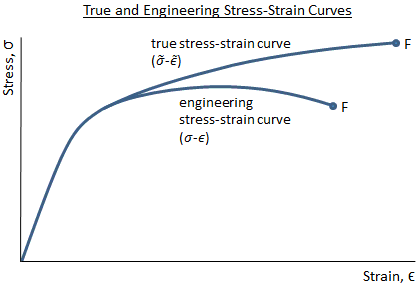
\includegraphics[width=0.6\textwidth]{images/true-stress-strain-diagram-01.png}
        \caption{True and engineering Stress and Strain curves (mechanicalc, 2024)}
        \label{fig:tvn}
    \end{figure}
    It should be noted that the engineering stress and the true stress are essentially the same in the linear-elastic region of the stress-strain curve. Because engineers typically operate within this linear-elastic region (it is uncommon to design a structure that is intended to operate beyond the elastic limit), it is valid to work with engineering stress as opposed to true stress.\\[8pt]
    \textbf{Engineering strain} is the change in length divided by the original length (See Eq. \ref{eq:strain}) Instead of just calculating a single value of $\Delta L$, consider that the change in length is divided among many small increments, $\Delta L_j$. The strain is also calculated in small increments:
    \begin{equation}
        \varepsilon_j = \frac{\Delta L_j}{L_j},
    \end{equation}
    where $\Delta L_j$ is the change in length for an increment, and $L_j$ is the length at the start of the increment. As these increments become infinitesimally small, the summation of the strains approaches the \textbf{true strain} ($\tilde{\varepsilon}$):
    \begin{equation}
        \tilde{\varepsilon} = \int_{L_0}^{L} \frac{dL}{L}=\ln\left(\frac{L}{L_0}\right)=\ln(1+\varepsilon)
    \end{equation}
    If it is assumed that the volume is constant throughout the deflection, then true stress and strain can be calculated as:
    \begin{align}
        \text{True Stress:} & \quad \tilde{\sigma} = \sigma \left( 1 + \varepsilon \right) \\
        \text{True Strain:} & \quad \tilde{\varepsilon} = \ln \left(\frac{A_0}{A}\right)
    \end{align}
    where $\tilde{\sigma}$ and $\tilde{\varepsilon}$ are the true stress and strain, and $\sigma$ and $\varepsilon$ are the engineering stress and strain.
    \newpage
    \subsection{Young's Modulus}
    \textbf{Young's Modulus} (\(E\)) (also known as \textit{Modulus of Elasticity}) defines the relationship between stress (\(\sigma\)) and strain (\(\varepsilon\)) as a linear fraction. It represents the rate at which stress leads to strain in a material and is determined from the tensile test within the elastic region. Mathematically, it is expressed as:
    \begin{equation}
        E = \frac{\sigma}{\varepsilon} 
        \label{eq:ym}
    \end{equation}
    \begin{itemize}[itemsep=-1mm]
        \item \( E \): Young's modulus (Pascals, Pa) or (Newtons per metre, \(\text{N/m}^2\)).
        \item \( \sigma \): Stress Pascals (Pascals, Pa) or (Newtons per metre, \(\text{N/m}^2\))
        \item \( \varepsilon \): Strain (no units).
    \end{itemize}    
    The formulas for stress (\( \sigma \)) (Eq. \ref{eq:stress}) and strain (\( \varepsilon \))(Eq. \ref{eq:strain}) can be used to expand the equation, and if needed, Eq. \ref{eq:deltaL} and Eq. \ref{eq:csa} can be incorporated for further elaboration. This can also be written as follows\footnote{Relevant units and variables are from the equations named, so i will not do an itemize for this}:
    \begin{equation}
        E = \frac{F \times L_0}{A\times\Delta L} = \frac{F \times L_0}{\left(w\times d\right)\left(L-L_0\right)}
    \end{equation}
{\begin{minipage}{0.5\textwidth}
    \begin{figure}[H]
        \centering
        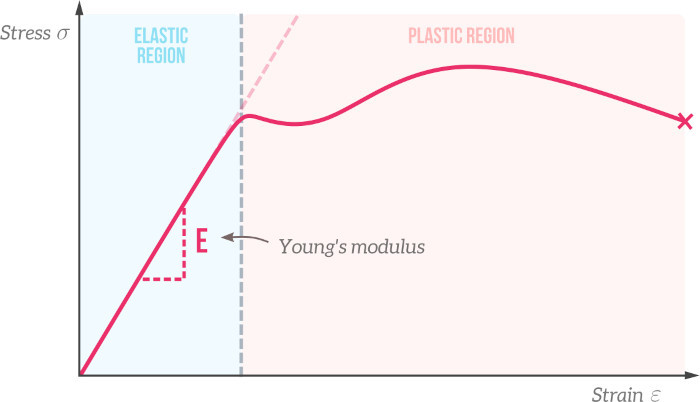
\includegraphics[width=1\textwidth]{images/stress-strain-youngs-modulus2.jpg}
        \caption{Stress and Strain graph showing Young's Modulus in the elastic region.}
        \label{fig:young}
    \end{figure}
\end{minipage}}\hspace{1em}
{\begin{minipage}{\dimexpr\textwidth-0.55\textwidth\relax}
    Young's Modulus ($E$) is a key material property that defines the relationship between stress ($\sigma$) and strain ($\varepsilon$) within the elastic range of a material's deformation. It indicates the stiffness of a material, showing how much strain will result from a specific stress.
    
    In a tensile test, Young's Modulus is calculated from the linear section of the stress-strain curve, 
\end{minipage}
known as the elastic region, where the material deforms in proportion to the applied load, as illustrated above (See Figure \ref{fig:young}).\\[8pt]  
In this region, the material will revert to its original shape once the load is removed, and the relationship between stress and strain remains linear.\\[8pt] 
Young's Modulus is significant because it quantifies a material's stiffness, which is crucial for selecting appropriate materials in engineering and construction.
\begin{itemize}
    \item \textbf{High }\(\bm{E}\): A higher Young's Modulus signifies that the material is stiffer, enabling it to resist deformation more effectively under stress. This characteristic is particularly beneficial in situations where minimal elastic deformation is essential, such as in the design of structural components or precision instruments.
    \item \textbf{Low }\(\bm{E}\): On the other hand, materials with a lower Young's Modulus are more flexible and may be better suited for applications that require compliance or the capacity to absorb energy.
\end{itemize}
    \newpage

    \subsection{Hooke's Law}
    One might see Hooke's law and be confused since this relates to springs, but here i show how the stress-strain, Young's modulus relationship interlinks with it. Hooke's law is an empirical law which states that the force needed to extend or compress a spring by some distance scales linearly with respect to that distance (Wikipedia, 2024).\\[8pt]
    In its simplest form, Hooke's Law states that:
    \begin{equation}
        F = kx
    \end{equation}
    Where:
    \begin{itemize}[itemsep=-1mm]
        \item $F$: Applied force (Newtons, N)
        \item $k$: Spring constant (Newtons per metre, N/m)
        \item $x$ Displacement (metres, m)
    \end{itemize}
    Note displacement is from equilibrium position\\[8pt] 
    This principle applies not only to springs but also to any elastic material. Here i prove such a thing, we begin with the stress-strain relationship, Young's Modulus (\(E\)) Eq. \ref{eq:ym} in tensile testing \footnote{Most equations presented here are meant only for derivation purposes (to prove my point). They consist of straightforward rearrangements and are not meant to be individually referenced at any particular point; hence, they are not numbered.}:    
    \[E = \frac{\sigma}{\varepsilon}\]
    \begin{center}
    Rearranging this equation to solve for stress (Multiply both sides by \(\varepsilon\)), we get:
    \[\sigma = E\varepsilon\]
    Next, we substitute the definition of stress as force (\(F\)) divided by the cross-sectional area (\(A\)):
    \[\frac{F}{A} = E\varepsilon\]
    To isolate the force (\(F\)), we multiply both sides by the cross-sectional area (\(A\)):
    \[F = A \times E\varepsilon\]
    Now, recall that strain (\(\varepsilon\)) is defined as the ratio of the change in length (\(\Delta L\)) to the original length (\(L_0\)):
    \[F = A \times E\frac{\Delta L}{L_0}\]
    Simplifying further, we get:
    \[F = \left(\frac{AE}{L_0}\right)\Delta L\]
    Since the cross-sectional area (\(A\)), Young's Modulus (\(E\)), and the original length (\(L_0\)) are constants, we can combine them into a new constant \(k = \frac{AE}{L_0}\), so the equation becomes:
    \begin{equation}
        F = k\Delta L
    \end{equation}
    Here, \(k = \frac{AE}{L_0}\) is the effective spring constant, which represents the material's resistance to deformation, analogous to the spring constant in Hooke's Law.    
    \end{center}
    \newpage



\begin{minipage}{0.52\textwidth}
This essentially proves that the extension (\(\Delta L\)) of the elongated body is proportional to the applied force (\(F\)), provided the limit of proportionality is not exceeded. 
\begin{equation}
    \Delta L \propto F
\end{equation}
This derivation demonstrates how Hooke's Law, typically associated with springs, applies to elastic materials in general.\\[8pt] 
However, it's crucial to understand the limitations and broader applications of this principle.
\begin{itemize}
    \item The law assumes a linear relationship between stress and strain, which holds true only in the elastic region (See Figure \ref{fig:young}).
\end{itemize}
\end{minipage}\hfill
\begin{minipage}{0.45\textwidth}
    \begin{figure}[H]
    \centering
    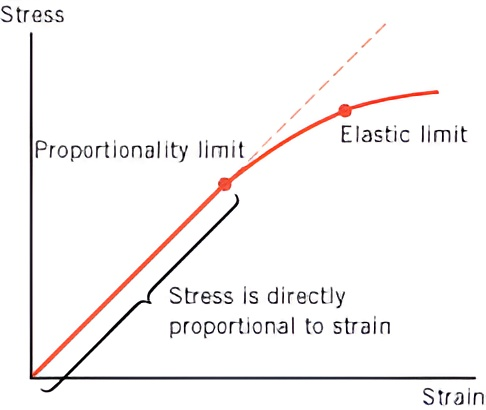
\includegraphics[width=0.87\textwidth]{images/hook(1).png}
    \caption{Illustration of the Stress-Strain Relationship Under Hooke’s Law}
    \label{fig:hook}
\end{figure}
\end{minipage}
\begin{itemize}
    \item In so, Hooke's Law is valid only within the elastic limit of a material, where deformation is reversible. Beyond this limit, permanent deformation occurs, and the stress-strain relationship becomes non-linear.
    \item Temperature significantly affects material properties, including Young's Modulus, altering material stiffness.
\end{itemize}
The linear behavior up to the elastic limit is due to the proportional stretching of atomic bonds relative to the applied force. This allows for reversible deformation. Beyond the elastic limit, atomic bonds begin to permanently deform, leading to plastic deformation and deviation from linearity (semanticscholar, 2017). \\[8pt]

Several misconceptions surround Hooke's Law, one of which is that materials react instantly to applied loads, adhering to Hooke's Law right away. In truth, many materials display time-dependent behaviors like \textbf{creep} (gradual deformation under constant stress) or \textbf{stress relaxation} (a decrease in stress under constant strain). These behaviors indicate that the straightforward, linear relationship outlined by Hooke's Law may not always represent the initial or only response of a material to applied forces. While I acknowledge this misconception, it will not be covered in depth in this report. \\[8pt]
A thorough understanding of Hooke's Law, its limitations, and its relationship with Young's Modulus is vital for effectively modeling and engineering material behavior across various applications.    
    
    \newpage
\subsection{Yield Point and Yield Strength}

 The \textbf{yield point} on a stress-strain curve marks the transition from elastic to plastic behavior. Below this point, the material deforms elastically and returns to its original shape when the stress is removed. Beyond this point, plastic deformation occurs, and some deformation becomes permanent.\\[8pt]
 The \textbf{yield strength} (\( \sigma_y \)) is the stress at the yield point and the corresponding strain called \textbf{yield strain} (\( \varepsilon_y \)). Mathematically, we can represent this point on the stress-strain curve as \( (\sigma_y,\ \varepsilon_y) \). To perform further calculations related to this point, such as the modulus of resilience (See Section \ref{mor}).\\[8pt]
This point marks the onset of plastic deformation. For materials like aluminum and cold-worked steel, which do not exhibit a distinct yield point due to a gradual transition to plastic deformation, the \textbf{offset yield point} (proof stress) is used. It is typically defined as 0.2\% of the strain within the proportionality limit, with the offset being from zero.\\[8pt] 
Yielding can be defined in several ways:\\
\begin{minipage}{0.4\textwidth}
     \begin{figure}[H]
     \centering
     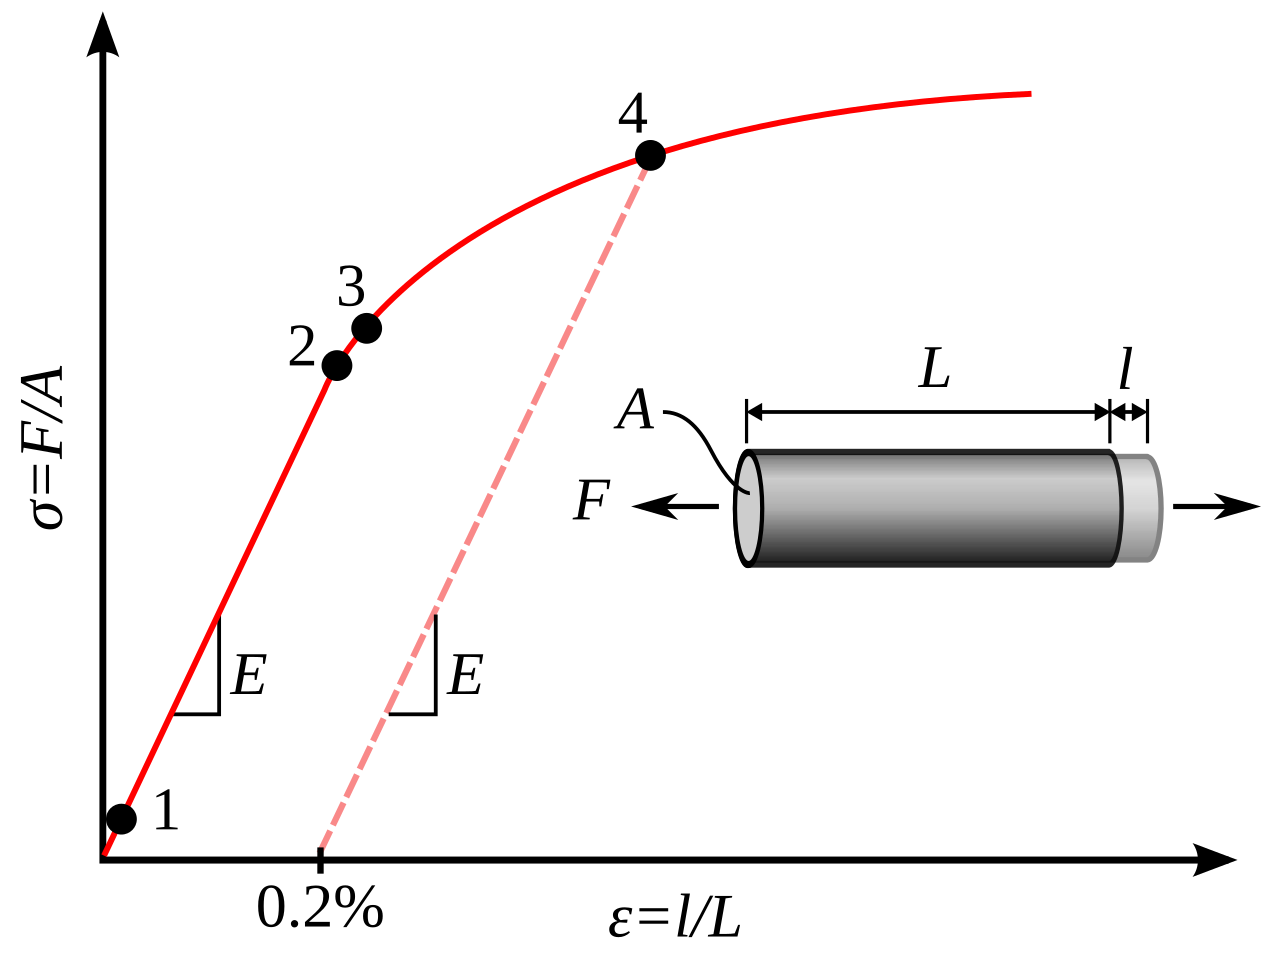
\includegraphics[width=1\textwidth]{images/Metal_yield.png}
     \caption{Stress–strain curve showing typical yield behavior for nonferrous alloys (stress (\(\sigma\)), shown as a function of strain (\(\epsilon\))) (Wikipedia, 2024)}
     \label{fig:str}
 \end{figure} 
 \end{minipage}\hfil
\begin{minipage}{0.6\textwidth}
 \begin{enumerate}
     \item \textbf{True elastic limit:} The lowest stress at which dislocations move. This definition is rarely used since dislocations move at very low stresses, and detecting such movement is very difficult (Wikipedia, 2024).
     \item \textbf{Proportionality Limit:} The point where stress is proportional to strain, corresponding to Hooke's law.
     \item \textbf{Elastic Limit (Yield Strength)}: The lowest stress at which permanent deformation occurs \((\sigma_y,\ \varepsilon_y)\).
     \item \textbf{Offset Yield Point (Proof Stress):} Used when no distinct yield point is observed, typically defined at 0.2\% plastic strain.
 \end{enumerate}
  \end{minipage}\\[8pt]
\textbf{Upper and Lower Yield Points:} For materials like mild steel, an upper yield point is followed by a drop to a lower yield point. The lower yield point is used for conservative design (Wikipedia, 2024).\\[8pt]
The \textbf{Elastic Limit (Yield Strength)} is important in determining the maximum allowable load a material can bear without permanent deformation. It is distinct from the \textit{ultimate tensile strength} (UTS), which is the maximum load a material can withstand before failure. For ductile materials, the ratio of yield strength to UTS is often used in applications like pipelines and is proportional to the strain hardening exponent shown in the ratio section (See Section \ref{}).
    
\newpage    

\subsection{Resilience and Modulus of Resilience}\label{mor}

The \textbf{modulus of resilience} is defined as the \textbf{maximum energy} absorbed \textbf{per unit volume} of a material due to straining up to the elastic limit. It represents the energy stored in the material when it deforms elastically, following Hooke's Law, without any permanent deformation. It is typically denoted as \( U_r \). Mathematically, the modulus of resilience is given by:

\begin{equation}
    U_r = \frac{\text{Proof Resilience}}{\text{Volume of the object}}
\end{equation}

Where proof resilience refers to the area under the stress-strain curve up to the elastic limit. To understand the modulus of resilience, it is important to first define \textbf{resilience} and \textbf{proof resilience}.

\begin{center}
\begin{minipage}[t]{0.46\textwidth}
\begin{figure}[H]
    \centering
    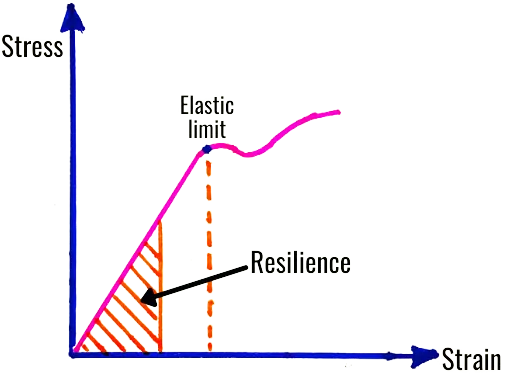
\includegraphics[width=0.87\textwidth]{images/resilience-1.png}
    \caption{resilience (mechcontent,2024)}
    \label{fig:resilience}
\end{figure}
\textbf{Resilience} is the \textbf{energy stored} in an object or specimen when it is strained below the elastic limit. More specifically, it is the strain energy stored in the object up to the elastic limit. It can also be described as the area under the load deflection curve up to the elastic limit (mechanicalc,2024;mechcontent,2024;testbook,2023).
\end{minipage}\hfil
\begin{minipage}[t]{0.46\textwidth}
\begin{figure}[H]
    \centering
    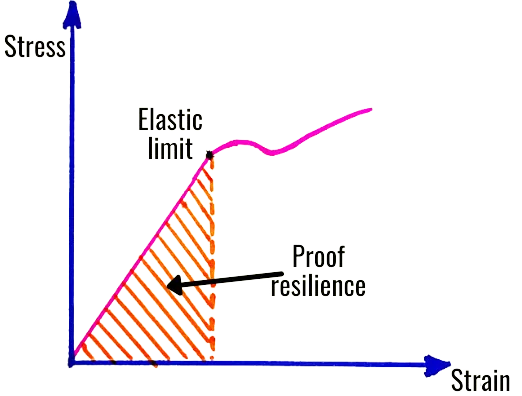
\includegraphics[width=0.87\textwidth]{images/proof-resilience-1.png}
    \caption{proof-resilience, (mechcontent,2024)}
    \label{fig:proof-resilience}
\end{figure}
\textbf{Proof resilience} is the \textbf{maximum value} of resilience, or the maximum amount of strain energy absorbed by the object up to the elastic limit. This energy does not cause permanent deformation. Proof resilience is also represented by the area under the stress-strain curve up to the elastic limit (mechcontent,2024;testbook,2023).
\end{minipage}

\end{center}

The \textbf{modulus of resilience} ($U_r$) quantifies the strain energy stored in a material up to its elastic limit. It is expressed as:
\begin{equation}
    U_r = \int_0^{\varepsilon_y} \sigma \, d\varepsilon
\end{equation}
In this equation, $\sigma$ represents the stress at a given strain $\varepsilon$, and $d\varepsilon$ is the infinitesimal change in strain. The integral sums the infinitesimal energy contributions $\sigma d\varepsilon$ from zero to the yield strain $\varepsilon_y$, which corresponds to the yield stress $\sigma_y$.\\[8pt]
\textbf{For materials exhibiting linear elastic behavior up to the yield point, the relationship between stress and strain is linear, and the integral can be simplified, else this is the general form.} 
\newpage
In this case, the area under the stress-strain curve up to the yield point (which is a triangle) gives the modulus of resilience:
\begin{equation}
    U_r = \frac{1}{2} \sigma_y \varepsilon_y
\end{equation}
\begin{itemize}[itemsep=-1mm]
    \item \(U_r\): Modulus of resilience (Joules per cubic meter, \( \text{J/m}^3 \)).
    \item \( \sigma_y \): {Yield stress} (Pascals, Pa) or (Newtons per meter squared, \( \text{N/m}^2 \))
    \item \( \varepsilon_y \): {Yield strain} (no units)
\end{itemize}
This represents the area of a triangle under the stress-strain curve, where \( \sigma_y \) is the yield stress and \( \varepsilon_y \) is the yield strain.\\[8pt]
Alternatively, using Young's modulus (\( E \)), the modulus of resilience can be written as:
\begin{equation}
    U_r = \frac{\sigma_y^2}{2E}
\end{equation}
Where:
\begin{itemize}[itemsep=-1mm]
    \item \( E \): {Young's modulus} (Pascals, Pa) or (Newtons per meter squared, \( \text{N/m}^2 \))
\end{itemize}
The formula represents the modulus of resilience, which is the maximum strain energy per unit volume that the material can store in the elastic region (up to the yield point) without permanent deformation. Volume does not explicitly appear because the modulus of resilience (\(U_r\)) is defined strain energy density, which is the strain energy per unit volume. This is equal to the area under the stress-strain diagram:  Stress (\(\sigma\)) and strain (\(\varepsilon\)) are normalized measures that inherently account for material dimensions, so their product directly yields energy density without needing to include volume in the formula.\\[8pt]
Off course for non-linear elastic materials, the area under the stress-strain curve up to the yield point must be calculated directly, as the simplified formulas may not apply.
\newpage    

\subsection{Ultimate Tensile Strength (UTS)}
Ultimate Tensile Strength (UTS) represents the maximum stress ($\sigma_{u}$) a material can withstand while being stretched before it breaks. It is determined from a stress-strain curve as the \textbf{peak stress value} prior to fracture and is crucial for ensuring safety in applications such as cables, bridges, and other load-bearing components. Its theoretical background is relatively straightforward compared to other material properties.\\[8pt]
It corresponds to the maximum force ($F_{\text{max}}$) applied relative to the original cross-sectional area ($A$) of the material. The equation for UTS is:
\begin{equation}
    \sigma_{u} = \frac{F_{\text{max}}}{A}
\end{equation}
\begin{itemize}[itemsep=-1mm]
    \item $\sigma_{u}$: Ultimate Tensile Strength (Mega Pascals, MPa)
    \item $F_{\text{max}}$: Maximum applied force (Newtons, N)
    \item $A$: Original cross-sectional area (metres squared, $\text{m}^2$)
\end{itemize}
In practical terms, UTS measures the maximum force per unit area a material can handle before failure. The value of UTS ($\sigma_{u}$) is observed directly from experimental data as the highest stress on a stress-strain curve. However, this equation is not always a useful analytical tool, as UTS is an observational property rather than a predictive one, especially since we typically use stress-strain relationships as the foundation for analysis.
\begin{center}
    \begin{minipage}{0.47\textwidth}\centering
        \begin{figure}[H]
            \centering
            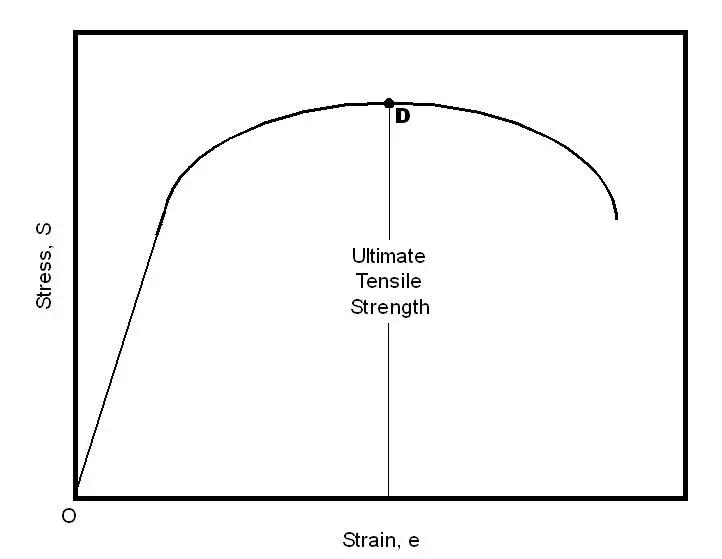
\includegraphics[width=0.9\textwidth]{images/ultimate-tensile-strength.png}
            \caption{Ultimate Tensile Strength (where point D is $\sigma_{u}$) (admet, 2024).}
            \label{fig:uts}
        \end{figure}
    \end{minipage}\hfil
    \begin{minipage}{0.45\textwidth}
        The UTS marks the transition where the material reaches its maximum load-bearing capacity before necking begins.\\[8pt] 
        After UTS, the material experiences localized deformation and ultimately fractures.\\[8pt]
        Ultimate Tensile Strength is commonly reported in units such as  Mega Pascals (MPa). These units are used because UTS values are typically large, making these units practical for communicating and comparing material performance.    
    \end{minipage}
\end{center}
Understanding the plastic behavior beyond UTS is essential for applications requiring high ductility and toughness, such as forming and shaping processes.


\newpage

\subsection{Ductility}\label{Ductility}
\begin{formal}[mechanicalc, 2024]
Ductility is an indication of how much plastic strain a material can withstand before it breaks. A ductile material can sustain large strains even after it has begun to yield. Common measures of ductility include percent elongation and reduction in area , as discussed in this section.
After a specimen breaks during a tensile test, the final length of the specimen is measured, and the \textbf{plastic strain at failure} $(\varepsilon_f)$, is calculated:
\begin{equation}
    \varepsilon_f = \frac{L_f - L_0}{L_0}
    \label{duc}
\end{equation}
\begin{itemize}[itemsep=-1mm]
    \item $\varepsilon_f$: Plastic strain at failure (no units)
    \item $L_0$: Original length (metres, m)
    \item $L_f$: Final length (metres, m)
\end{itemize}
It is important to note that after the specimen breaks, the elastic strain that existed while the specimen was under load is recovered. Therefore, the measured difference between the final and initial lengths gives the plastic strain at failure (mechanicalc, 2024). This is illustrated in the figure below:\\[8pt]
\begin{minipage}{0.45\textwidth}\centering
    \begin{figure}[H]
    \centering
    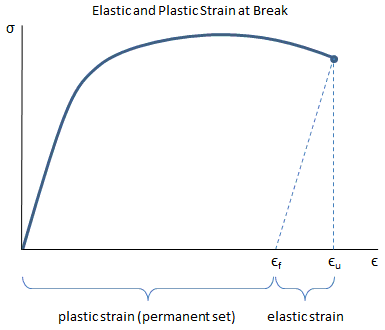
\includegraphics[width=1.1\textwidth]{images/elastic-plastic-strain-at-break-01.png}
    \caption{Elastic and Plastic Strain at Break (mechanicalc, 2024).}
    \label{fig:strain-break}
\end{figure}
\end{minipage}\hfill
\begin{minipage}{0.49\textwidth}
In the figure, it can be seen that the plastic strain at failure, is the strain remaining in the material after the elastic strain has been recovered.\\[8pt]
The \textbf{percent elongation} \((eL)\) is calculated from the plastic strain at failure by:
\begin{equation}
    eL = \varepsilon_f \times 100\% = \frac{L_f - L_0}{L_0} \times 100\%
    \label{el}
\end{equation}
\begin{itemize}[itemsep=-1mm]
    \item $eL$: Percent elongation (Percent, \%)
\end{itemize}
The percent elongation is a commonly provided material property, so the plastic strain at failure is typically calculated from the percent elongation:
\begin{equation}
    \varepsilon_f = \frac{eL}{100\%}
\end{equation}
\end{minipage}\\[8pt]
The \textbf{ultimate strain} $(\varepsilon_u)$ accounts for both plastic and elastic strain at failure, representing the total strain at failure as the sum of the plastic strain and the elastic strain:
\begin{equation}
    \varepsilon_u = \varepsilon_f + \frac{\sigma_{u}}{E}
    \label{useless}
\end{equation}
\begin{itemize}[itemsep=-1mm]
    \item $\varepsilon_u$: Ultimate strain (No units)
    \item $\sigma_{u}$: Ultimate stress (Pascals, Pa) or (Newtons per metre, \(\text{N/m}^2\))
    \item $E$: Young's modulus (Pascals, Pa) or (Newtons per metre, \(\text{N/m}^2\))
\end{itemize} 
\end{formal}
\newpage
While \ref{useless} provides a theoretical relationship between ultimate strain, plastic strain at failure, ultimate stress, and Young's modulus, its practical utility is limited because ultimate strain is typically measured directly from experimental data rather than calculated\\[8pt]
The stress at the ultimate strain is known as the \textbf{Fracture Stress} \((\sigma_f)\) represents the stress at the point where the material breaks. It is typically less than the Ultimate Tensile Strength (UTS) for ductile materials because the material continues to deform plastically after reaching UTS but before fracturing.\\[8pt]
Another important material property that can be measured during a tensile test is the reduction in area, which is calculated by:
\begin{equation}
    \text{Reduction in Area} = \frac{A_0 - A_f}{A_0} \times 100\%
\end{equation}
\begin{itemize}[itemsep=-1mm]
    \item $A_0$ Original cross-sectional area
    \item $A_f$ Cross-sectional area after fracture
\end{itemize}
Again units are only relevant in ensuring that the Reduction in Area percentage is dimensionless or properly represented as a percentage. It is also important to remember that percent elongation and reduction in area account for the plastic components of the axial strain and the lateral strain, respectively.\\



    \newpage

\subsection{Toughness and Modulus of Toughness}

\textbf{Toughness} is a material's ability to absorb energy up to the point of fracture, combining strength and ductility. In material science, toughness is typically determined as the area under the load vs deflection curve, which represents the energy absorbed by the material.\\[8pt]
\begin{formal}[mechanicalc, 2024]
    The \textbf{modulus of toughness} quantifies the strain energy density a material can absorb just before fracturing, calculated from the total area under the stress-strain curve up to the point of fracture. It can be approximated by dividing the stress-strain curve into triangular and rectangular sections, with the height being the average of the yield and ultimate strengths.
\begin{center}
    \begin{minipage}{0.5\textwidth}\centering
        \begin{figure}[H]
            \centering
            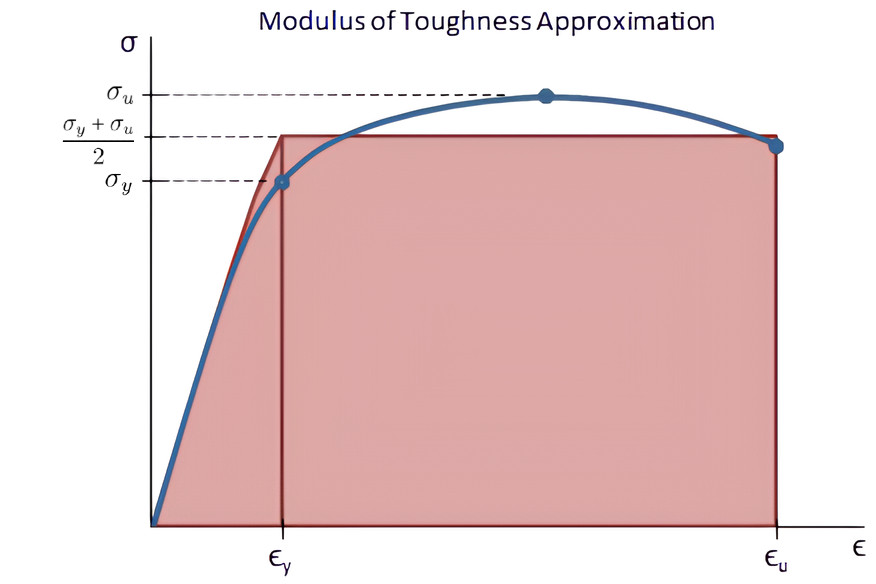
\includegraphics[width=1\textwidth]{images/modulus-of-toughness-approx-01(1).jpg}
            \caption{modulus-of-toughness-approx (mechanicalc, 2024)}
            \label{fig:mot}
        \end{figure}
    \end{minipage}\hfil
    \begin{minipage}{0.45\textwidth}
        \begin{equation}
            \begin{aligned}
                U_t &\approx \left(\frac{\sigma_{y} + \sigma_{u}}{2}\right)\times\left(\varepsilon_u - \frac{\varepsilon_y}{2}\right)\\
                &\approx \varepsilon_u\left(\frac{\sigma_{y} + \sigma_{u}}{2}\right) -\frac{1}{2E}\left(\frac{\sigma_{y} + \sigma_{u}}{2}\right)^2
            \end{aligned}
        \end{equation}
        Where:
        \begin{itemize}[left=0pt, itemsep=-1mm]
            \item \( U_t \): Modulus of toughness (Pascals, Pa)
            \item $\sigma_y$: Tensile yield strength (Pascals, Pa)
            \item $\sigma_u$: Tensile ultimate strength (Pascals, Pa)
            \item $\varepsilon_y$: Strain at yield (no units)
            \item $\varepsilon_u$: Ultimate strain (no units)
            \item $E$: Elastic modulus (Pascals, Pa)
        \end{itemize}
    \end{minipage}
\end{center}
For a more accurate calculation, the \textbf{Ramberg-Osgood equation} can be used to approximate the stress-strain curve, followed by integration to find the area under the curve.\\[8pt]
The plastic region (rectangular portion) of the stress-strain curve significantly contributes to toughness. Ductile materials can withstand more plastic strain than brittle ones, so they exhibit a higher modulus of toughness, even with the same yield strength. While structures are designed to keep stresses within the elastic region, ductile materials with a higher modulus of toughness are better suited for applications involving accidental overloads.
\end{formal}

\newpage

\subsection{Material Property Ratios}\label{mpr}
\vspace{0.5em}
\begin{enumerate}
    
    \item \textbf{Strength Ratio}:\\[8pt]
    \begin{minipage}{0.3\textwidth}
        \begin{equation}
            \frac{\sigma_u}{\sigma_y}
        \end{equation}
    \end{minipage}\hfill
    \begin{minipage}{0.6\textwidth}
        This ratio compares the ultimate tensile strength (\(\sigma_u\)) to the yield strength (\(\sigma_y\)), providing an idea of how much additional strain a material can take beyond the yield point before failure.
    \end{minipage}
    
    \item \textbf{Strain Ratio}:\\[8pt]
    \begin{minipage}{0.3\textwidth}
        \begin{equation}
            \frac{\varepsilon_u}{\varepsilon_y}
        \end{equation}
    \end{minipage}\hfill
    \begin{minipage}{0.6\textwidth}
        This ratio compares the ultimate strain (\(\varepsilon_u\)) to the strain at yield (\(\varepsilon_y\)), reflecting how much plastic deformation a material can undergo compared to its initial elastic deformation.
    \end{minipage}
    
    \item \textbf{Toughness-to-Resilience Ratio}:\\[8pt]
    \begin{minipage}{0.3\textwidth}
        \begin{equation}
            \frac{U_t}{U_r}
        \end{equation}
    \end{minipage}\hfill
    \begin{minipage}{0.6\textwidth}
        This ratio compares the modulus of toughness (energy absorbed before fracture) to the modulus of resilience (energy absorbed without permanent deformation), providing insight into the material's energy absorption capacity.
    \end{minipage}
    
    \item \textbf{Fracture-to-UTS Stress Ratio}:\\[8pt]
    \begin{minipage}{0.3\textwidth}
        \begin{equation}
            \frac{\sigma_f}{\sigma_u}
        \end{equation}
    \end{minipage}\hfill
    \begin{minipage}{0.6\textwidth}
        This ratio compares the fracture stress (\(\sigma_f\)) to the ultimate tensile strength (\(\sigma_u\)), indicating how much higher the material's ultimate strength is compared to the fracture strength.
    \end{minipage}
    
\end{enumerate}
\vspace{1em}
\textbf{Note:} While there are many other material property ratios that can be derived, we focus here on these four key ratios due to their relevance in understanding the fundamental mechanical behavior of materials. Other ratios, such as the Young’s Modulus to Yield Strength ratio or the Slimness ratio, may provide useful insights but are beyond the scope of this discussion.

        
    \newpage\vspace*{-20pt}
    
    \section{Data, Calculations and Results}
    
    While the tensile test provides valuable information about a material's strength and ductility, there are certain parameters that cannot be directly derived or accurately measured in this specific test setup. These limitations include:
    \begin{itemize}[left=0pt, itemsep=-1mm]
        \item \textbf{Reduction in Area:} The reduction in area, which measures the change in cross-sectional area at the point of fracture, cannot be directly determined in this test setup as the fracture point and necking behavior are not fully captured i.e they weren't measured.
        \item \textbf{True Stress and True Strain:} The calculation of true stress and true strain requires continuous measurement of the specimen's dimensions during deformation. In this case, only engineering stress and strain are measured, which are based on the original dimensions of the specimen and do not account for changes in geometry during deformation.
    \end{itemize}
    As a result, certain material properties that rely on these parameters are not directly available from the current tensile test data. Regardless we move on with the analysis.\\
    \vspace{1em}
    \hrule
    \vspace{1em}
    Now that we have collected the following data:
    \begin{itemize}
        \item Hardness (HV5)
        \item Gauge [Width (\(w\)), Thickness (\(d\)), Length (\(L_0\))]
        \item Corresponding set of values of Forces \((F)\) that relate to a specific Change in Length \((\Delta L)\).
    \end{itemize}
    We can derive several mechanical properties from the test data. The properties outlined in the theory section include:
    \begin{itemize}
        \item Cross-Sectional Area ($A_0$)
        \item Stress ($\sigma$) and Strain ($\varepsilon$)
        \item Stiffness ($k$) and Young's Modulus ($E$)
        \item \textbf{Yield point:} Yield Strength ($\sigma_y$) and Yield Strain ($\varepsilon_y$)
        \item Resilience ($U_r$) and Toughness ($U_t$)
        \item Ultimate Strength ($\sigma_u$)
        \item \textbf{Fracture point:} Ultimate Strain ($\varepsilon_u$) and Fracture Stress ($\sigma_f$)
        \item Plastic Strain at Failure ($\varepsilon_f$) and Percent Elongation ($eL$)  
        \item Material Property Ratios
    \end{itemize}
    These derived properties help us fully characterize the mechanical performance of the material under stress. \textbf{All interpretations of results are included in the Discussion Section.}
    \newpage
    \subsection{Hardness}\label{meanhard}
    While we've gone over the important equations for the Vickers hardness test, in this prior theory section (See Section \ref{VHC}) there's no need to actually do the calculations by hand since the machine has already provided the results. I hope this much is clear by now.\\[8pt] 
    The data recorded in Table \ref{tab:hv5} is outlined as such:\vspace{1em}
    \begin{center}
        \begin{tblr}{
                width=\textwidth,
                colspec={X[3,c]X[0.75,c]X[0.75,c]X[0.75,c]X[0.75,c]X[0.75,c]X[0.75,c]X[0.8,c]X[0.8,c]X[0.8,c]},
                hlines,vlines,
                rows={ht=1\baselineskip},
                row{1} = {ht=1\baselineskip,font=\bfseries,c,m},
                cells={valign=m,halign=c}
            }
            Property (\(\bm{\text{unitless}}\)) & \SetCell[c=2]{c} AR & & \SetCell[c=2]{c} ST & & \SetCell[c=3]{c} PH & & \\
            HV5 (Individual) & 119 & 123 & 36 & 36.8 & 102.8 & 131 & 126 \\
        \end{tblr}
    \end{center}\vspace{1em}
    To calculate the mean (or average) for each set of values, 
    sum all individual values and divide by the total number of values, as shown by the formula:
    \begin{equation}
        \text{Mean} = \frac{\sum x_i}{n}
    \end{equation}
    Where:
    \begin{itemize}[itemsep=-1mm]
        \item \textbf{Mean}: The arithmetic average, representing the central tendency of the dataset.
        \item \( x_i \): Each individual value in the dataset.
        \item \( n \): The total number of values in the dataset.
        \item \( \sum x_i \): The sum of all individual values.
    \end{itemize}
    Before calculating the mean, it is important to identify and remove outliers. 
    During the lab, it was determined that the value \textbf{102.8 from PH was an outlier}. With this adjustment, the results can now proceed as follows:\\
    \begin{center}
    \begin{minipage}{0.3\textwidth}\centering
            \textbf{AR:}
            \[\sum x_i = 119 + 123 = 242\]
            \[n = 2 \; \Rightarrow \; \text{Mean} = \frac{242}{2} = 121\]
    \end{minipage}\hspace{0.8em}\vrule\hspace{0.8em}
    \begin{minipage}{0.3\textwidth}\centering
        \textbf{ST:}
        \[\sum x_i = 36 + 36.8 = 72.8\]
        \[n = 2 \; \Rightarrow \; \text{Mean} = \frac{72.8}{2} = 36.4\]
    \end{minipage}\hspace{0.8em}\vrule\hspace{0.8em}
    \begin{minipage}{0.3\textwidth}\centering    
        \textbf{PH:}
        \[\sum x_i = 131 + 126 = 257\]
        \[n = 2 \; \Rightarrow \; \text{Mean} = \frac{257}{2} = 128.5\]
    \end{minipage}
    \end{center}    
    Thus, the means for each group are as follows:\vspace{1em}
        \begin{table}[H]
            \centering
            \begin{tblr}{
                    width=\textwidth,
                    colspec={X[3,c]X[1,c]X[1,c]X[1,c]},
                    hlines,vlines,
                    rows={ht=1\baselineskip},
                    row{1} = {ht=1\baselineskip,font=\bfseries,c,m},
                    cells={valign=m,halign=c}
                }
                Property (\(\bm{\text{unitless}}\)) & AR & ST & PH \\
                HV5 (Average) & 121 & 36.4 & 128.5 \\
            \end{tblr}
            \caption{HV5 individual and mean data}
            \label{tab:hv5mean}
        \end{table}
        
    Honestly this is pretty much it for the hardness test we got our individual and averages there's not much else we can do with this.
    \newpage
    
        \subsection{Cross-Sectional Areas (CSA)}
        
        \begin{center}
        \begin{minipage}{0.3\textwidth} 
            \centering
            \begin{tikzpicture}[rotate around y=225, use Hobby shortcut, scale=0.25, every node/.style={scale=0.25}]
                \large
                \def\width{4}
                \def\gap{10}
                \def\main{8}
                \def\curvy{1.9}
                \def\depth{3}
                
                \def\n{3.3}
                \def\z{1/\n}
                \pgfmathsetmacro{\s}{1-\z}
                
                \coordinate (A) at (0,\main,0);
                \coordinate (B) at (\width*\z-\width*\z*0.23,\main+\curvy-\curvy*0.7,0);
                \coordinate (C) at (\width*\z,\main+\curvy,0);
                
                \coordinate (A2) at (\width,\main,0);
                \coordinate (B2) at (\width*\s+\width*\z*0.23,\main+\curvy-\curvy*0.7,0);
                \coordinate (C2) at (\width*\s,\main+\curvy,0);
                
                \coordinate (A3) at (0,\main+\gap,0);
                \coordinate (B3) at (\width*\z-\width*\z*0.23,\main+\gap-\curvy+\curvy*0.7,0);
                \coordinate (C3) at (\width*\z,\main+\gap-\curvy,0);
                
                \coordinate (A4) at (\width,\main+\gap,0);
                \coordinate (B4) at (\width*\s+\width*\z*0.23,\main+\gap-\curvy+\curvy*0.7,0);
                \coordinate (C4) at (\width*\s,\main+\gap-\curvy,0);
                
                % Back variation with \depth (subtracting \depth from the z-coordinate)
                \coordinate (A') at (0,\main,\depth);
                \coordinate (B') at (\width*\z-\width*\z*0.23,\main+\curvy-\curvy*0.7,\depth);
                \coordinate (C') at (\width*\z,\main+\curvy,\depth);
                
                \coordinate (A2') at (\width,\main,\depth);
                \coordinate (B2') at (\width*\s+\width*\z*0.23,\main+\curvy-\curvy*0.7,\depth);
                \coordinate (C2') at (\width*\s,\main+\curvy,\depth);
                
                \coordinate (A3') at (0,\main+\gap,\depth);
                \coordinate (B3') at (\width*\z-\width*\z*0.23,\main+\gap-\curvy+\curvy*0.7,\depth);
                \coordinate (C3') at (\width*\z,\main+\gap-\curvy,\depth);
                
                \coordinate (A4') at (\width,\main+\gap,\depth);
                \coordinate (B4') at (\width*\s+\width*\z*0.23,\main+\gap-\curvy+\curvy*0.7,\depth);
                \coordinate (C4') at (\width*\s,\main+\gap-\curvy,\depth);
                
                
                % Back face fill
                \fill[black!40] 
                (0,0,\depth) -- (\width,0,\depth) -- (\width,\main,\depth) 
                to[hobby,tension=3] (\width,\main,\depth) .. (\width*\s+\width*\z*0.23,\main+\curvy-\curvy*0.7,\depth) .. (\width*\s,\main+\curvy,\depth) -- 
                (\width*\s,\main+\gap-\curvy,\depth) 
                to[hobby,tension=3] (\width*\s,\main+\gap-\curvy,\depth)  .. (\width*\s+\width*\z*0.23,\main+\gap-\curvy+\curvy*0.7,\depth) .. (\width,\main+\gap,\depth) --
                (\width,2*\main+\gap,\depth) -- (0,2*\main+\gap,\depth) -- 
                (0,\main+\gap,\depth) to[hobby,tension=3] (0,\main+\gap,\depth) .. (\width*\z-\width*\z*0.23,\main+\gap-\curvy+\curvy*0.7,\depth) .. (\width*\z,\main+\gap-\curvy,\depth) --
                (\width*\z,\main+\curvy,\depth) to[hobby,tension=3] (\width*\z,\main+\curvy,\depth) .. (\width*\z-\width*\z*0.23,\main+\curvy-\curvy*0.7,\depth) .. (0,\main,\depth) --
                cycle;
                
                % Curves fills with refined fades
                \fill[left color=gray!80, middle color=gray!50, right color=gray!20, opacity=0.8] 
                (A) to[hobby,tension=3] (A) .. (B) .. (C) -- (C3) to[hobby,tension=3] (C3) .. (B3) .. (A3) -- 
                (A3') to[hobby,tension=3] (A3') .. (B3') .. (C3') --
                (C') to[hobby,tension=3] (C') .. (B') .. (A') -- cycle;
                
                \fill[left color=gray!80, middle color=gray!50, right color=gray!20, opacity=0.8] 
                (A2) to[hobby,tension=3] (A2) .. (B2) .. (C2) -- (C4) to[hobby,tension=3] (C4) .. (B4) .. (A4) -- 
                (A4') to[hobby,tension=3] (A4') .. (B4') .. (C4') --
                (C2') to[hobby,tension=3] (C2') .. (B2') .. (A2') -- cycle;
                
                
                \draw[-,hobby,tension=3] (A2') .. (B2') .. (C2');
                \draw[-,hobby,tension=3] (A4') .. (B4') .. (C4');
                
                % Fill for bottom rectangle section
                \fill[black!33] 
                (0,0,0) -- (\width,0,0) -- (\width,0,\depth) -- (0,0,\depth) -- cycle;
                \fill[black!33] 
                (0,0,0) -- (0,\main,0) -- (0,\main,\depth) -- (0,0,\depth) -- cycle;
                \fill[black!40] 
                (\width,0,0) -- (\width,\main,0) -- (\width,\main,\depth) -- (\width,0,\depth) -- cycle;
                
                % Fill for top rectangle section
                \fill[black!30] 
                (0,2*\main+\gap,0) -- (\width,2*\main+\gap,0) -- (\width,2*\main+\gap,\depth) -- (0,2*\main+\gap,\depth) -- cycle;
                \fill[black!30] 
                (0,\main+\gap,0) -- (0,2*\main+\gap,0) -- (0,2*\main+\gap,\depth) -- (0,\main+\gap,\depth) -- cycle;
                \fill[black!33] 
                (\width,\main+\gap,0) -- (\width,2*\main+\gap,0) -- (\width,2*\main+\gap,\depth) -- (\width,\main+\gap,\depth) -- cycle;
                
                
                
                % Front face fill
                \fill[black!36] 
                (0,0,0) -- (\width,0,0) -- (\width,\main,0) 
                to[hobby,tension=3] (A2) .. (B2) .. (C2) -- 
                (\width*\s,\main+\gap-\curvy,0) 
                to[hobby,tension=3] (C4) .. (B4) .. (A4) --
                (\width,2*\main+\gap,0) -- (0,2*\main+\gap,0) -- 
                (0,\main+\gap,0) to[hobby,tension=3] (A3) .. (B3) .. (C3) --
                (\width*\z,\main+\curvy,0) to[hobby,tension=3] (C) .. (B) .. (A) --
                cycle;
                \draw[hobby,tension=3] (A) .. (B) .. (C);
                \draw[hobby,tension=3] (A2) .. (B2) .. (C2);
                \draw[hobby,tension=3] (A3) .. (B3) .. (C3);
                \draw[hobby,tension=3] (A4) .. (B4) .. (C4);
                \draw[dashed, opacity=0.3,hobby,tension=3] (A3') .. (B3') .. (C3');
                \draw[dashed, opacity=0.3,hobby,tension=3] (A') .. (B') .. (C');
                % Front face outline
                
                \draw[-] (0,0,0) -- (\width,0,0);
                \draw[-] (0,0,0) -- (0,\main,0);
                \draw[-] (\width*\z,\main+\curvy,0) -- (\width*\z,\main+\gap-\curvy,0);
                \draw[-] (0,\main+\gap,0) -- (0,2*\main+\gap,0);
                \draw[-] (0,2*\main+\gap,0) -- (\width,2*\main+\gap,0);
                \draw[-] (\width,2*\main+\gap,0) -- (\width,\main+\gap,0);
                \draw[-] (\width*\s,\main+\curvy,0) -- (\width*\s,\main+\gap-\curvy,0);    
                \draw[-] (\width,0,0) -- (\width,\main,0);
                
                
                
                
                
                % Back face outline
                
                
                \draw[dashed, opacity=0.3] (\width*\z,\main+\curvy,\depth) -- (\width*\z,\main+\gap-\curvy,\depth);
                \draw[-] (\width*\s,\main+\curvy,\depth) -- (\width*\s,\main+\gap-\curvy,\depth);
                \draw[dashed, opacity=0.3] (0,0,\depth) -- (\width,0,\depth);
                \draw[dashed, opacity=0.3] (0,0,\depth) -- (0,\main,\depth);
                \draw[-] (\width,0,\depth) -- (\width,\main,\depth);
                \draw[dashed, opacity=0.3] (0,\main+\gap,\depth) -- (0,2*\main+\gap,\depth);
                \draw[-] (0,2*\main+\gap,\depth) -- (\width,2*\main+\gap,\depth);
                \draw[-] (\width,2*\main+\gap,\depth) -- (\width,\main+\gap,\depth);
                
                
                
                % Connect front and back faces
                %botom
                \draw[-] (\width,\main,0) -- (\width,\main,\depth);
                \draw[-] (\width,0,0) -- (\width,0,\depth);
                \draw[dashed, opacity=0.3] (0,0,0) -- (0,0,\depth);
                \draw[-] (0,\main,0) -- (0,\main,\depth);
                %top
                \draw[-] (\width,\main+\gap,0) -- (\width,\main+\gap,\depth);
                \draw[-] (\width,2*\main+\gap,0) -- (\width,2*\main+\gap,\depth);
                \draw[-] (0,2*\main+\gap,0) -- (0,2*\main+\gap,\depth);
                \draw[dashed, opacity=0.3] (0,\main+\gap,0) -- (0,\main+\gap,\depth);
                
                
                
                %curves
                \draw[dashed, opacity=0.3] (C) -- (C2);
                \draw[dashed, opacity=0.3] (C3) -- (C4);
                \draw[dashed, opacity=0.3] (C') -- (C2');
                \draw[dashed, opacity=0.3] (C3') -- (C4');
                \draw[dashed, opacity=0.3] (C) -- (C');
                \draw[dashed, opacity=0.3] (C2) -- (C2');
                \draw[dashed, opacity=0.3] (C3) -- (C3');
                \draw[dashed, opacity=0.3] (C4) -- (C4');
                
                
                \fill[opacity=0.6,pattern={Lines[
                    distance=1mm,
                    angle=45,
                    line width=0.4mm
                    ]},
                pattern color=blue
                ] (C2) -- (C) -- (C3) -- (C4) -- cycle;
                
            \end{tikzpicture}\\
            \color{blue} \textbf{\textsf{CSA 1}}
        \end{minipage}\hspace{-1em}
        \begin{minipage}{0.3\textwidth}
            \centering
            \begin{tikzpicture}[rotate around y=225, use Hobby shortcut, scale=0.25, every node/.style={scale=0.25}]
                \large
                \def\width{4}
                \def\gap{10}
                \def\main{8}
                \def\curvy{1.9}
                \def\depth{3}
                
                \def\n{3.3}
                \def\z{1/\n}
                \pgfmathsetmacro{\s}{1-\z}
                
                \coordinate (A) at (0,\main,0);
                \coordinate (B) at (\width*\z-\width*\z*0.23,\main+\curvy-\curvy*0.7,0);
                \coordinate (C) at (\width*\z,\main+\curvy,0);
                
                \coordinate (A2) at (\width,\main,0);
                \coordinate (B2) at (\width*\s+\width*\z*0.23,\main+\curvy-\curvy*0.7,0);
                \coordinate (C2) at (\width*\s,\main+\curvy,0);
                
                \coordinate (A3) at (0,\main+\gap,0);
                \coordinate (B3) at (\width*\z-\width*\z*0.23,\main+\gap-\curvy+\curvy*0.7,0);
                \coordinate (C3) at (\width*\z,\main+\gap-\curvy,0);
                
                \coordinate (A4) at (\width,\main+\gap,0);
                \coordinate (B4) at (\width*\s+\width*\z*0.23,\main+\gap-\curvy+\curvy*0.7,0);
                \coordinate (C4) at (\width*\s,\main+\gap-\curvy,0);
                
                % Back variation with \depth (subtracting \depth from the z-coordinate)
                \coordinate (A') at (0,\main,\depth);
                \coordinate (B') at (\width*\z-\width*\z*0.23,\main+\curvy-\curvy*0.7,\depth);
                \coordinate (C') at (\width*\z,\main+\curvy,\depth);
                
                \coordinate (A2') at (\width,\main,\depth);
                \coordinate (B2') at (\width*\s+\width*\z*0.23,\main+\curvy-\curvy*0.7,\depth);
                \coordinate (C2') at (\width*\s,\main+\curvy,\depth);
                
                \coordinate (A3') at (0,\main+\gap,\depth);
                \coordinate (B3') at (\width*\z-\width*\z*0.23,\main+\gap-\curvy+\curvy*0.7,\depth);
                \coordinate (C3') at (\width*\z,\main+\gap-\curvy,\depth);
                
                \coordinate (A4') at (\width,\main+\gap,\depth);
                \coordinate (B4') at (\width*\s+\width*\z*0.23,\main+\gap-\curvy+\curvy*0.7,\depth);
                \coordinate (C4') at (\width*\s,\main+\gap-\curvy,\depth);
                
                
                % Back face fill
                \fill[black!40] 
                (0,0,\depth) -- (\width,0,\depth) -- (\width,\main,\depth) 
                to[hobby,tension=3] (\width,\main,\depth) .. (\width*\s+\width*\z*0.23,\main+\curvy-\curvy*0.7,\depth) .. (\width*\s,\main+\curvy,\depth) -- 
                (\width*\s,\main+\gap-\curvy,\depth) 
                to[hobby,tension=3] (\width*\s,\main+\gap-\curvy,\depth)  .. (\width*\s+\width*\z*0.23,\main+\gap-\curvy+\curvy*0.7,\depth) .. (\width,\main+\gap,\depth) --
                (\width,2*\main+\gap,\depth) -- (0,2*\main+\gap,\depth) -- 
                (0,\main+\gap,\depth) to[hobby,tension=3] (0,\main+\gap,\depth) .. (\width*\z-\width*\z*0.23,\main+\gap-\curvy+\curvy*0.7,\depth) .. (\width*\z,\main+\gap-\curvy,\depth) --
                (\width*\z,\main+\curvy,\depth) to[hobby,tension=3] (\width*\z,\main+\curvy,\depth) .. (\width*\z-\width*\z*0.23,\main+\curvy-\curvy*0.7,\depth) .. (0,\main,\depth) --
                cycle;
                
                % Curves fills with refined fades
                \fill[left color=gray!80, middle color=gray!50, right color=gray!20, opacity=0.8] 
                (A) to[hobby,tension=3] (A) .. (B) .. (C) -- (C3) to[hobby,tension=3] (C3) .. (B3) .. (A3) -- 
                (A3') to[hobby,tension=3] (A3') .. (B3') .. (C3') --
                (C') to[hobby,tension=3] (C') .. (B') .. (A') -- cycle;
                
                \fill[left color=gray!80, middle color=gray!50, right color=gray!20, opacity=0.8] 
                (A2) to[hobby,tension=3] (A2) .. (B2) .. (C2) -- (C4) to[hobby,tension=3] (C4) .. (B4) .. (A4) -- 
                (A4') to[hobby,tension=3] (A4') .. (B4') .. (C4') --
                (C2') to[hobby,tension=3] (C2') .. (B2') .. (A2') -- cycle;
                
                
                \draw[-,hobby,tension=3] (A2') .. (B2') .. (C2');
                \draw[-,hobby,tension=3] (A4') .. (B4') .. (C4');
                
                % Fill for bottom rectangle section
                \fill[black!33] 
                (0,0,0) -- (\width,0,0) -- (\width,0,\depth) -- (0,0,\depth) -- cycle;
                \fill[black!33] 
                (0,0,0) -- (0,\main,0) -- (0,\main,\depth) -- (0,0,\depth) -- cycle;
                \fill[black!40] 
                (\width,0,0) -- (\width,\main,0) -- (\width,\main,\depth) -- (\width,0,\depth) -- cycle;
                
                % Fill for top rectangle section
                \fill[black!30] 
                (0,2*\main+\gap,0) -- (\width,2*\main+\gap,0) -- (\width,2*\main+\gap,\depth) -- (0,2*\main+\gap,\depth) -- cycle;
                \fill[black!30] 
                (0,\main+\gap,0) -- (0,2*\main+\gap,0) -- (0,2*\main+\gap,\depth) -- (0,\main+\gap,\depth) -- cycle;
                \fill[black!33] 
                (\width,\main+\gap,0) -- (\width,2*\main+\gap,0) -- (\width,2*\main+\gap,\depth) -- (\width,\main+\gap,\depth) -- cycle;
                
                
                
                % Front face fill
                \fill[black!36] 
                (0,0,0) -- (\width,0,0) -- (\width,\main,0) 
                to[hobby,tension=3] (A2) .. (B2) .. (C2) -- 
                (\width*\s,\main+\gap-\curvy,0) 
                to[hobby,tension=3] (C4) .. (B4) .. (A4) --
                (\width,2*\main+\gap,0) -- (0,2*\main+\gap,0) -- 
                (0,\main+\gap,0) to[hobby,tension=3] (A3) .. (B3) .. (C3) --
                (\width*\z,\main+\curvy,0) to[hobby,tension=3] (C) .. (B) .. (A) --
                cycle;
                \draw[hobby,tension=3] (A) .. (B) .. (C);
                \draw[hobby,tension=3] (A2) .. (B2) .. (C2);
                \draw[hobby,tension=3] (A3) .. (B3) .. (C3);
                \draw[hobby,tension=3] (A4) .. (B4) .. (C4);
                \draw[dashed, opacity=0.3,hobby,tension=3] (A3') .. (B3') .. (C3');
                \draw[dashed, opacity=0.3,hobby,tension=3] (A') .. (B') .. (C');
                % Front face outline
                
                \draw[-] (0,0,0) -- (\width,0,0);
                \draw[-] (0,0,0) -- (0,\main,0);
                \draw[-] (\width*\z,\main+\curvy,0) -- (\width*\z,\main+\gap-\curvy,0);
                \draw[-] (0,\main+\gap,0) -- (0,2*\main+\gap,0);
                \draw[-] (0,2*\main+\gap,0) -- (\width,2*\main+\gap,0);
                \draw[-] (\width,2*\main+\gap,0) -- (\width,\main+\gap,0);
                \draw[-] (\width*\s,\main+\curvy,0) -- (\width*\s,\main+\gap-\curvy,0);    
                \draw[-] (\width,0,0) -- (\width,\main,0);
                
                
                
                
                
                % Back face outline
                
                
                \draw[dashed, opacity=0.3] (\width*\z,\main+\curvy,\depth) -- (\width*\z,\main+\gap-\curvy,\depth);
                \draw[-] (\width*\s,\main+\curvy,\depth) -- (\width*\s,\main+\gap-\curvy,\depth);
                \draw[dashed, opacity=0.3] (0,0,\depth) -- (\width,0,\depth);
                \draw[dashed, opacity=0.3] (0,0,\depth) -- (0,\main,\depth);
                \draw[-] (\width,0,\depth) -- (\width,\main,\depth);
                \draw[dashed, opacity=0.3] (0,\main+\gap,\depth) -- (0,2*\main+\gap,\depth);
                \draw[-] (0,2*\main+\gap,\depth) -- (\width,2*\main+\gap,\depth);
                \draw[-] (\width,2*\main+\gap,\depth) -- (\width,\main+\gap,\depth);
                
                
                
                % Connect front and back faces
                %botom
                \draw[-] (\width,\main,0) -- (\width,\main,\depth);
                \draw[-] (\width,0,0) -- (\width,0,\depth);
                \draw[dashed, opacity=0.3] (0,0,0) -- (0,0,\depth);
                \draw[-] (0,\main,0) -- (0,\main,\depth);
                %top
                \draw[-] (\width,\main+\gap,0) -- (\width,\main+\gap,\depth);
                \draw[-] (\width,2*\main+\gap,0) -- (\width,2*\main+\gap,\depth);
                \draw[-] (0,2*\main+\gap,0) -- (0,2*\main+\gap,\depth);
                \draw[dashed, opacity=0.3] (0,\main+\gap,0) -- (0,\main+\gap,\depth);
                
                
                
                %curves
                \draw[dashed, opacity=0.3] (C) -- (C2);
                \draw[dashed, opacity=0.3] (C3) -- (C4);
                \draw[dashed, opacity=0.3] (C') -- (C2');
                \draw[dashed, opacity=0.3] (C3') -- (C4');
                \draw[dashed, opacity=0.3] (C) -- (C');
                \draw[dashed, opacity=0.3] (C2) -- (C2');
                \draw[dashed, opacity=0.3] (C3) -- (C3');
                \draw[dashed, opacity=0.3] (C4) -- (C4');
                
                
                \fill[opacity=0.6,pattern={Lines[
                    distance=1mm,
                    angle=45,
                    line width=0.4mm
                    ]},
                pattern color=green!70!black
                ] (C2) -- (C4) -- (C4') -- (C2') -- cycle;
            \end{tikzpicture}\\    
            \color{green!50!black} \textbf{\textsf{CSA 2}}
        \end{minipage}\hspace{-1em}
        \begin{minipage}{0.3\textwidth}
            \centering
            \begin{tikzpicture}[rotate around y=225, use Hobby shortcut, scale=0.25, every node/.style={scale=0.25}]
                \large
                \def\width{4}
                \def\gap{10}
                \def\main{8}
                \def\curvy{1.9}
                \def\depth{3}
                
                \def\n{3.3}
                \def\z{1/\n}
                \pgfmathsetmacro{\s}{1-\z}
                
                \coordinate (A) at (0,\main,0);
                \coordinate (B) at (\width*\z-\width*\z*0.23,\main+\curvy-\curvy*0.7,0);
                \coordinate (C) at (\width*\z,\main+\curvy,0);
                
                \coordinate (A2) at (\width,\main,0);
                \coordinate (B2) at (\width*\s+\width*\z*0.23,\main+\curvy-\curvy*0.7,0);
                \coordinate (C2) at (\width*\s,\main+\curvy,0);
                
                \coordinate (A3) at (0,\main+\gap,0);
                \coordinate (B3) at (\width*\z-\width*\z*0.23,\main+\gap-\curvy+\curvy*0.7,0);
                \coordinate (C3) at (\width*\z,\main+\gap-\curvy,0);
                
                \coordinate (A4) at (\width,\main+\gap,0);
                \coordinate (B4) at (\width*\s+\width*\z*0.23,\main+\gap-\curvy+\curvy*0.7,0);
                \coordinate (C4) at (\width*\s,\main+\gap-\curvy,0);
                
                % Back variation with \depth (subtracting \depth from the z-coordinate)
                \coordinate (A') at (0,\main,\depth);
                \coordinate (B') at (\width*\z-\width*\z*0.23,\main+\curvy-\curvy*0.7,\depth);
                \coordinate (C') at (\width*\z,\main+\curvy,\depth);
                
                \coordinate (A2') at (\width,\main,\depth);
                \coordinate (B2') at (\width*\s+\width*\z*0.23,\main+\curvy-\curvy*0.7,\depth);
                \coordinate (C2') at (\width*\s,\main+\curvy,\depth);
                
                \coordinate (A3') at (0,\main+\gap,\depth);
                \coordinate (B3') at (\width*\z-\width*\z*0.23,\main+\gap-\curvy+\curvy*0.7,\depth);
                \coordinate (C3') at (\width*\z,\main+\gap-\curvy,\depth);
                
                \coordinate (A4') at (\width,\main+\gap,\depth);
                \coordinate (B4') at (\width*\s+\width*\z*0.23,\main+\gap-\curvy+\curvy*0.7,\depth);
                \coordinate (C4') at (\width*\s,\main+\gap-\curvy,\depth);
                
                
                % Back face fill
                \fill[black!40] 
                (0,0,\depth) -- (\width,0,\depth) -- (\width,\main,\depth) 
                to[hobby,tension=3] (\width,\main,\depth) .. (\width*\s+\width*\z*0.23,\main+\curvy-\curvy*0.7,\depth) .. (\width*\s,\main+\curvy,\depth) -- 
                (\width*\s,\main+\gap-\curvy,\depth) 
                to[hobby,tension=3] (\width*\s,\main+\gap-\curvy,\depth)  .. (\width*\s+\width*\z*0.23,\main+\gap-\curvy+\curvy*0.7,\depth) .. (\width,\main+\gap,\depth) --
                (\width,2*\main+\gap,\depth) -- (0,2*\main+\gap,\depth) -- 
                (0,\main+\gap,\depth) to[hobby,tension=3] (0,\main+\gap,\depth) .. (\width*\z-\width*\z*0.23,\main+\gap-\curvy+\curvy*0.7,\depth) .. (\width*\z,\main+\gap-\curvy,\depth) --
                (\width*\z,\main+\curvy,\depth) to[hobby,tension=3] (\width*\z,\main+\curvy,\depth) .. (\width*\z-\width*\z*0.23,\main+\curvy-\curvy*0.7,\depth) .. (0,\main,\depth) --
                cycle;
                
                % Curves fills with refined fades
                \fill[left color=gray!80, middle color=gray!50, right color=gray!20, opacity=0.8] 
                (A) to[hobby,tension=3] (A) .. (B) .. (C) -- (C3) to[hobby,tension=3] (C3) .. (B3) .. (A3) -- 
                (A3') to[hobby,tension=3] (A3') .. (B3') .. (C3') --
                (C') to[hobby,tension=3] (C') .. (B') .. (A') -- cycle;
                
                \fill[left color=gray!80, middle color=gray!50, right color=gray!20, opacity=0.8] 
                (A2) to[hobby,tension=3] (A2) .. (B2) .. (C2) -- (C4) to[hobby,tension=3] (C4) .. (B4) .. (A4) -- 
                (A4') to[hobby,tension=3] (A4') .. (B4') .. (C4') --
                (C2') to[hobby,tension=3] (C2') .. (B2') .. (A2') -- cycle;
                
                
                \draw[-,hobby,tension=3] (A2') .. (B2') .. (C2');
                \draw[-,hobby,tension=3] (A4') .. (B4') .. (C4');
                
                % Fill for bottom rectangle section
                \fill[black!33] 
                (0,0,0) -- (\width,0,0) -- (\width,0,\depth) -- (0,0,\depth) -- cycle;
                \fill[black!33] 
                (0,0,0) -- (0,\main,0) -- (0,\main,\depth) -- (0,0,\depth) -- cycle;
                \fill[black!40] 
                (\width,0,0) -- (\width,\main,0) -- (\width,\main,\depth) -- (\width,0,\depth) -- cycle;
                
                % Fill for top rectangle section
                \fill[black!30] 
                (0,2*\main+\gap,0) -- (\width,2*\main+\gap,0) -- (\width,2*\main+\gap,\depth) -- (0,2*\main+\gap,\depth) -- cycle;
                \fill[black!30] 
                (0,\main+\gap,0) -- (0,2*\main+\gap,0) -- (0,2*\main+\gap,\depth) -- (0,\main+\gap,\depth) -- cycle;
                \fill[black!33] 
                (\width,\main+\gap,0) -- (\width,2*\main+\gap,0) -- (\width,2*\main+\gap,\depth) -- (\width,\main+\gap,\depth) -- cycle;
                
                
                
                % Front face fill
                \fill[black!36] 
                (0,0,0) -- (\width,0,0) -- (\width,\main,0) 
                to[hobby,tension=3] (A2) .. (B2) .. (C2) -- 
                (\width*\s,\main+\gap-\curvy,0) 
                to[hobby,tension=3] (C4) .. (B4) .. (A4) --
                (\width,2*\main+\gap,0) -- (0,2*\main+\gap,0) -- 
                (0,\main+\gap,0) to[hobby,tension=3] (A3) .. (B3) .. (C3) --
                (\width*\z,\main+\curvy,0) to[hobby,tension=3] (C) .. (B) .. (A) --
                cycle;
                \draw[hobby,tension=3] (A) .. (B) .. (C);
                \draw[hobby,tension=3] (A2) .. (B2) .. (C2);
                \draw[hobby,tension=3] (A3) .. (B3) .. (C3);
                \draw[hobby,tension=3] (A4) .. (B4) .. (C4);
                \draw[dashed, opacity=0.3,hobby,tension=3] (A3') .. (B3') .. (C3');
                \draw[dashed, opacity=0.3,hobby,tension=3] (A') .. (B') .. (C');
                % Front face outline
                
                \draw[-] (0,0,0) -- (\width,0,0);
                \draw[-] (0,0,0) -- (0,\main,0);
                \draw[-] (\width*\z,\main+\curvy,0) -- (\width*\z,\main+\gap-\curvy,0);
                \draw[-] (0,\main+\gap,0) -- (0,2*\main+\gap,0);
                \draw[-] (0,2*\main+\gap,0) -- (\width,2*\main+\gap,0);
                \draw[-] (\width,2*\main+\gap,0) -- (\width,\main+\gap,0);
                \draw[-] (\width*\s,\main+\curvy,0) -- (\width*\s,\main+\gap-\curvy,0);    
                \draw[-] (\width,0,0) -- (\width,\main,0);
                
                
                
                
                
                % Back face outline
                
                
                \draw[dashed, opacity=0.3] (\width*\z,\main+\curvy,\depth) -- (\width*\z,\main+\gap-\curvy,\depth);
                \draw[-] (\width*\s,\main+\curvy,\depth) -- (\width*\s,\main+\gap-\curvy,\depth);
                \draw[dashed, opacity=0.3] (0,0,\depth) -- (\width,0,\depth);
                \draw[dashed, opacity=0.3] (0,0,\depth) -- (0,\main,\depth);
                \draw[-] (\width,0,\depth) -- (\width,\main,\depth);
                \draw[dashed, opacity=0.3] (0,\main+\gap,\depth) -- (0,2*\main+\gap,\depth);
                \draw[-] (0,2*\main+\gap,\depth) -- (\width,2*\main+\gap,\depth);
                \draw[-] (\width,2*\main+\gap,\depth) -- (\width,\main+\gap,\depth);
                
                
                
                % Connect front and back faces
                %botom
                \draw[-] (\width,\main,0) -- (\width,\main,\depth);
                \draw[-] (\width,0,0) -- (\width,0,\depth);
                \draw[dashed, opacity=0.3] (0,0,0) -- (0,0,\depth);
                \draw[-] (0,\main,0) -- (0,\main,\depth);
                %top
                \draw[-] (\width,\main+\gap,0) -- (\width,\main+\gap,\depth);
                \draw[-] (\width,2*\main+\gap,0) -- (\width,2*\main+\gap,\depth);
                \draw[-] (0,2*\main+\gap,0) -- (0,2*\main+\gap,\depth);
                \draw[dashed, opacity=0.3] (0,\main+\gap,0) -- (0,\main+\gap,\depth);
                
                
                
                %curves
                \draw[dashed, opacity=0.3] (C) -- (C2);
                \draw[dashed, opacity=0.3] (C3) -- (C4);
                \draw[dashed, opacity=0.3] (C') -- (C2');
                \draw[dashed, opacity=0.3] (C3') -- (C4');
                \draw[dashed, opacity=0.3] (C) -- (C');
                \draw[dashed, opacity=0.3] (C2) -- (C2');
                \draw[dashed, opacity=0.3] (C3) -- (C3');
                \draw[dashed, opacity=0.3] (C4) -- (C4');
                
                \pgfmathsetmacro{\halfgap}{0.5*\gap}
                
                \coordinate (C3m) at (\width*\z,\main+\halfgap,0);
                \coordinate (C4m) at (\width*\s,\main+\halfgap,0);
                \coordinate (C3'm) at (\width*\z,\main+\halfgap,\depth);
                \coordinate (C4'm) at (\width*\s,\main+\halfgap,\depth);
                
                \fill[pattern={Lines[
                    distance=1mm,
                    angle=45,
                    line width=0.4mm
                    ]},
                pattern color=red,
                opacity=0.6] (C3m) -- (C3'm) -- (C4'm) -- (C4m) -- cycle;
            \end{tikzpicture}\\
            \color{red} \textbf{\textsf{CSA 3}}
        \end{minipage}\\[1em]

            \begin{tblr}{
                    width=\textwidth,
                    colspec={X[2.9,c]X[1.5,c]X[1.5,c]X[1.6,c]},
                    hlines,vlines,
                    rows={ht=1.5\baselineskip},
                    row{1} = {ht=1\baselineskip,font=\bfseries,c,m},
                    cells={valign=m,halign=c}
                }
                Property ($\bm{\text{mm}^2}$) & AR & ST & PH\\
                {\color{blue} \textbf{\textsf{CSA 1}} \\ Width \(\times\) Length} 
                & {\(11.98 \times 50\) \\ \(= 599\)} 
                & {\(12 \times 50\) \\ \(= 600\)} 
                & {\(11.97 \times 50\) \\ \(= 598.5\)} \\
                {\color{green!50!black} \textbf{\textsf{CSA 2}} \\ Thickness \(\times\) Length} 
                & {\(6 \times 50\) \\ \(= 300\)} 
                & {\(6.38 \times 50\) \\ \(= 319\)} 
                & {\(6.18 \times 50\) \\ \(= 309\)} \\
                {\color{red} \textbf{\textsf{CSA 3}} \\ Width \(\times\) Thickness} 
                & {\(11.98 \times 6\) \\ \(= 71.88\)} 
                & {\(12 \times 6.38\) \\ \(= 76.56\)} 
                & {\(11.97 \times 6.18\) \\ \(= 73.96\)} \\
            \end{tblr}
            \captionof{table}{Calculated Cross-Sectional Areas (CSA) for AR, ST, and PH (Dimensions from Table \ref{tab:dimensions})}
            \label{tab:csa}
        \end{center}
        In a tensile test, force is applied from the top and bottom of the alloy, stretching it along its length. Stress is calculated as the force divided by the area \textbf{perpendicular} to the applied force (See Eq. \ref{eq:stress}). Thus, the appropriate cross-sectional area for stress calculation is the one that is orthogonal to this force.
    \begin{itemize}[left=0pt,itemsep=-0.3mm]
        \item \textbf{\textcolor{blue}{\textsf{CSA 1}}:} This CSA parameterizes the thickness dimension of the alloy and remains coplanar with the applied force vector, rendering it unsuitable for stress calculations.
        \item \textbf{\textcolor{green!50!black}{\textsf{CSA 2}}:} This CSA parameterizes the width dimension and also remains coplanar with the applied force vector, thus it is not utilized for stress calculations.
        \item \textbf{\textcolor{red}{\textsf{CSA 3}}:} This CSA parameterizes the longitudinal dimension of the material and maintains orthogonality to the applied force vector, making it the appropriate choice for stress calculations.
    \end{itemize}
    Thus, for stress calculations, we use \textbf{CSA 3}, as it is the area perpendicular to the applied force. The table below shows the calculated cross section area values for which is to be used.
    \begin{center}
        \begin{tblr}{
               width=\textwidth,
                colspec={X[3.5,c]X[1,c]X[1,c]X[1,c]},
                hlines,vlines,
                rows={ht=1.3\baselineskip},
                row{1} = {ht=0.9\baselineskip,font=\bfseries,c,m},
                cells={valign=m,halign=c}
                }
            Property  & AR & ST & PH\\
        \(\textbf{Cross-Sectional Area}\ (\bm{A_0})\ (\text{mm}^2)\) & 71.88 & 76.56 & 73.97 \\
        \end{tblr}
        \captionof{table}{Cross-Sectional Area (CSA) to be used for stress}
        \label{tab:csa3}
    \end{center}

    This data will be used in subsequent calculations for stress and other related analyses.
    \newpage
    
    \subsection{Force vs Displacement}
        The data from the A4 sheet printed by the machine (see Figure \ref{fig:tensile_results}) has been revised for clarity by eliminating unnecessary details. The table, graph axes, and titles have been reformatted to improve readability.
        \renewcommand{\arraystretch}{1.4}
        \begin{table}[H]
            \centering
            \begin{tblr}{
                    colspec={X[1,c]X[2,c]X[2,c]},
                    hlines,vlines,
                    cells={valign=m,halign=c}
                }
                \textbf{Specimen ID} & \(\textbf{Maximum Load}\ \bm{(F_{max})}\ \text{(N)}\) & \(\textbf{Extension at Break}\ \bm{(\Delta L_f)}\ \text{(mm)}\) \\
                \textcolor{red}{ST} & 8580 & 19.8 \\
                \textcolor{green!50!black}{PH} & 23800 & 9.8 \\
                \textcolor{blue}{AR} & 24400 & 9.7 \\
                \end{tblr}
            \caption{Relevant extracted data from the table (See Figure \ref{fig:tensile_results})}
            \label{tab:specimen_data}
        \end{table}
    \begin{figure}[H]
        \centering
        \includegraphics[width=0.8\textwidth]{figures/force_vs_elongation.png}        \caption{Machine produced data for Force vs Change in Length}
        \label{fig:force_elong}
    \end{figure}
   The data was reconstructed into CSV files using automeris.io, as the original data file was not given. The graph was subsequently plotted using Matplotlib.
   
 \subsection{Stress vs. Strain}
 
 The transition from Force vs Change in Length to Stress vs Strain is a critical step in analyzing the mechanical properties of materials. This section explains the process and the utilization of code to perform this transformation.\\[8pt]
 The Force vs Change in Length graph (Figure \ref{fig:force_elong}) shows the direct relationship between the applied load and the change in length of the specimen. This raw data is essential but lacks the normalization required for comparative analysis. To gain a deeper understanding of the material's behavior, the raw data must be transformed into stress and strain. This normalization process involves the following steps:
 \begin{enumerate}
     \item \textbf{Calculating Stress}: Stress is defined as the force per unit area (See Eq. \ref{eq:stress}). This normalizes the force data, making it independent of the specimen's size.
     \item \textbf{Calculating Strain}: Strain is the change in length relative to the original length (See Eq. \ref{eq:strain}). This normalizes the elongation data, providing a dimensionless measure of deformation.
 \end{enumerate}
 The transformation from Force vs. Elongation to Stress vs. Strain was achieved using a Python script. The script performs the following key steps:
 \begin{enumerate}
     \item \textbf{Loading Data}: The raw data for each specimen is loaded from CSV\footnotemark files.
     \item \textbf{Defining Constants}: The original gauge length and cross-sectional areas for each specimen are defined.
     \item \textbf{Calculating Stress and Strain}: The script calculates stress and strain for each data point using the formulas mentioned above.
     \item \textbf{Storing the Stress and Strain}: We then store the stress and strain for each data point into new CSV files.
     \item \textbf{Plotting the Data}: The transformed data is plotted to visualize the Stress vs. Strain relationship.
 \end{enumerate}
 The resulting Stress vs. Strain graph (Figure \ref{fig:stress_strain}) provides a standardized and comparable representation of the material's behavior under tensile loading.\\\noindent\footnotetext{"A CSV (comma-separated values) file is a plain text file that stores data in a table-structured format, with commas separating values and newlines separating records. CSV files are commonly used to transfer large amounts of data between programs with little to no user reformatting"}    \newpage
 \begin{figure}[H]
     \centering
     \includegraphics[width=0.8\textwidth]{figures/stress_vs_strain.png}
     \caption{Calculated produced data for Stress vs. Strain}
     \label{fig:stress_strain}
 \end{figure} 
 The transition from Force vs. Elongation to Stress vs. Strain is essential for understanding and comparing the mechanical properties of materials. By normalizing the raw data, we obtain a more universal and meaningful representation of material behavior. The utilization of code streamlines this transformation process, ensuring accuracy and efficiency in data analysis.\\[8pt] 
 Let's now define the attributes now that we have our baseline.
   \newpage
\subsection{Young's Modulus}

Young's Modulus, also known as the modulus of elasticity, is a measure of the stiffness of a material. It is defined as the slope of the stress-strain curve in the linear elastic region. In this section, i describe the methodology used to calculate Young's Modulus for each specimen and present the results.\\[8pt]

\textbf{Methodology}\\[8pt]

To calculate Young's Modulus, i performed linear regression\footnote{In statistics, linear regression is a model that estimates the linear relationship between a scalar response and one or more explanatory variables. A model with exactly one explanatory variable is a simple linear regression; a model with two or more explanatory variables is a multiple linear regression. (Wikipedia,2024)} on a specified strain range within the stress-strain data. The strain range was chosen to ensure that the material behavior is linear and elastic. The following steps were taken:

\begin{enumerate}
    \item \textbf{Loading Data}: The stress and strain data for each specimen were loaded from previously created CSV files.
    \item \textbf{Defining Strain Range}: A specific strain range was defined for each specimen to ensure linear elastic behavior.
    \item \textbf{Linear Regression}: Linear regression was performed on the data points within the specified strain range to calculate the slope, which represents Young's Modulus.
    \item \textbf{Plotting}: The stress vs. strain data and the fitted line for Young's Modulus were plotted for each specimen.
\end{enumerate}
\newpage
\textbf{Specimen Analysis and Results}\\[8pt]
The strain range used for calculating Young's Modulus was chosen to ensure that the material behavior is linear and elastic:  
\begin{itemize}
    \item \textbf{Specimen AR \& PH}: The strain range selected for calculating Young's Modulus is from 10\% to 40\% of the total strain. This range excludes the initial region of the stress-strain curve, where a slight curvature is observed. The curvature at the start likely arises from initial imperfections in the setup, such as slack in the specimen or the grips, or minor adjustments during the early stages of loading. These effects can introduce non-linearity that does not reflect the true elastic behavior of the material.
    \item \textbf{Specimen ST}: The strain range selected for calculating Young's Modulus is from 0\% to 10\% of the total strain. Unlike Specimens AR and PH, the stress-strain curve for Specimen ST begins with a distinct linear region but transitions to non-linear behavior at a much lower strain value. This early deviation from linearity indicates that the material’s elastic region is more limited compared to the other specimens.
\end{itemize}
\vspace{1em}
\begin{minipage}[t]{0.3\textwidth}
    \centering
    \includegraphics[width=\textwidth]{figures/stress_vs_strain_with_fit_AR.png}
    \captionof{figure}{\(E\) fit for {alloy AR}}
    \label{fig:stress_strain_AR}
\end{minipage}%
\hfill%
\begin{minipage}[t]{0.3\textwidth}
    \centering
    \includegraphics[width=\textwidth]{figures/stress_vs_strain_with_fit_ST.png}
    \captionof{figure}{\(E\) fit for {alloy PH}}
    \label{fig:stress_strain_PH}
\end{minipage}%
\hfill%
\begin{minipage}[t]{0.3\textwidth}
    \centering
    \includegraphics[width=\textwidth]{figures/stress_vs_strain_with_fit_PH.png}
    \captionof{figure}{\(E\) fit for {alloy ST}}
    \label{fig:stress_strain_ST}
\end{minipage}\\[8pt]
The calculated Young's Modulus for all specimens is summarized below:
\begin{table}[H]
    \centering
    \begin{tblr}{
            width=\textwidth,
            colspec={X[3.5,c]X[1,c]X[1,c]X[1,c]},
            hlines,vlines,
            rows={ht=1.3\baselineskip},
            row{1} = {ht=0.9\baselineskip,font=\bfseries,c,m},
            cells={valign=m,halign=c}
        }
        Property & \textbf{AR} & \textbf{ST} & \textbf{PH} \\
        \(\textbf{Young's Modulus}\ (\bm{E})\ (\text{N/}\text{mm}^2)\) & 5522.83 & 1850.18 & 5154.74 \\
    \end{tblr}
    \caption{{Young's Modulus for Each Specimen}}
    \label{tab:youngs_modulus}
\end{table}
\vspace{1em}\noindent
\newpage
\subsection{Stiffness}
The stiffness is the effective spring constant, which represents the material's resistance to deformation. We derived \( k \), the stiffness, in the Hooke's Law section as follows:
\begin{equation}
    k = \frac{AE}{L_0}
\end{equation}
Given the data collected for Young's Modulus \( E \) (See Table \ref{tab:youngs_modulus}), original length \( L_0 \) (See Table \ref{tab:dimensions}), and original cross-sectional area \( A_0 \) (See Table \ref{tab:csa3}), we summarize and combine the relevant data:\vspace{-1em}
\begin{center}
    \begin{tblr}{
            width=\textwidth,
            colspec={X[3.5,c]X[1,c]X[1,c]X[1,c]},
            hlines,vlines,
            rows={ht=1.3\baselineskip},
            row{1} = {ht=0.9\baselineskip,font=\bfseries,c,m},
            cells={valign=m,halign=c}
        }
        Property & AR & ST & PH \\
        \(\textbf{Young's Modulus}\ (\bm{E})\ (\text{N/}\text{mm}^2)\) & 5522.83 & 1850.18 & 5154.74 \\
        \(\textbf{Cross-Sectional Area}\ (\bm{A_0})\ (\text{mm}^2)\) & 71.88 & 76.56 & 73.97 \\
        \(\textbf{Original Length}\ (\bm{L_0})\ (\text{mm})\) & 50 & 50 & 50 \\
    \end{tblr}
\end{center}
We perform the calculations as follows:\\[8pt]

    \begin{minipage}{1.1\textwidth}    \hspace{-1em}
    \begin{minipage}{0.3\textwidth}\centering
    \textbf{AR:}
    \begin{align*}
        k &= \frac{71.88 \, \text{mm}^2 \times 5522.83 \, \text{N/}\text{mm}^2}{50 \, \text{mm}} \\
        &\approx 7939.6 \, \text{N/mm or kN/m}
    \end{align*}
\end{minipage}\hspace{0.5em}\vrule\hspace{0.5em}
\begin{minipage}{0.3\textwidth}\centering
    \textbf{ST:}
    \begin{align*}
        k &= \frac{76.56 \, \text{mm}^2 \times 1850.18 \, \text{N/}\text{mm}^2}{50 \, \text{mm}} \\
        &\approx 2833 \, \text{N/mm or kN/m}
    \end{align*}
\end{minipage}\hspace{0.5em}\vrule\hspace{0.5em}
\begin{minipage}{0.3\textwidth}\centering
    \textbf{PH:}
    \begin{align*}
        k &= \frac{73.97 \, \text{mm}^2 \times 5154.74 \, \text{N/}\text{mm}^2}{50 \, \text{mm}} \\
        &\approx 7625.9 \, \text{N/mm or kN/m}
    \end{align*}
\end{minipage}
\end{minipage}\\[10pt]
These calculations provide the stiffness for each specimen, which is a crucial parameter in understanding the material's resistance to deformation under applied loads, summarised results are in the table below:\vspace{-1em}
\begin{center}
    \begin{tblr}{
            width=\textwidth,
            colspec={X[3.5,c]X[1,c]X[1,c]X[1,c]},
            hlines,vlines,
            rows={ht=1.3\baselineskip},
            row{1} = {ht=0.9\baselineskip,font=\bfseries,c,m},
            cells={valign=m,halign=c}
        }
        Property & AR & ST & PH \\
        \(\textbf{Stiffness}\ (\bm{k})\ (\text{N/mm or kN/m})\) & 7939.6 & 2833 & 7625.9 \\
    \end{tblr}
    \captionof{table}{Stiffness for Each Specimen}
    \label{tab:stiffness}
\end{center}
\newpage
\subsection{Yield Point}
Given that the \(E\)-line is already plotted alongside the respective curves for Specimens AR, ST, and PH in Figures \ref{fig:stress_strain_AR}, \ref{fig:stress_strain_ST}, and \ref{fig:stress_strain_PH}, I simply made an appropriate observation-based choice for each specimen.\\[8pt]
\begin{minipage}[t]{0.3\textwidth}
    \centering
    \includegraphics[width=\textwidth]{figures/stress_vs_strain_with_fit_ARand_yield.png}
    \captionof{figure}{yield point for {alloy AR}}
    \label{fig:stress_strain_AR_y}
\end{minipage}%
\hfill%
\begin{minipage}[t]{0.3\textwidth}
    \centering
    \includegraphics[width=\textwidth]{figures/stress_vs_strain_with_fit_STand_yield.png}
    \captionof{figure}{yield point  for {alloy PH}}
    \label{fig:stress_strain_PH_y}
\end{minipage}%
\hfill%
\begin{minipage}[t]{0.3\textwidth}
    \centering
    \includegraphics[width=\textwidth]{figures/stress_vs_strain_with_fit_PHand_yield.png}
    \captionof{figure}{yield point for {Specimen ST}}
    \label{fig:stress_strain_ST_y}
\end{minipage}\\[8pt]
The observed yield point for all specimens is summarized below:
\begin{table}[H]
    \centering
    \begin{tblr}{
            width=\textwidth,
            colspec={X[3.5,c]X[1,c]X[1,c]X[1,c]},
            hlines,vlines,
            rows={ht=1.3\baselineskip},
            row{1} = {ht=0.9\baselineskip,font=\bfseries,c,m},
            cells={valign=m,halign=c}
        }
        Property & AR & ST & PH \\
        \(\textbf{Yield Strain}\ \bm{(\varepsilon_y)}\ (\text{no units})\) & 0.068 & 0.024 & 0.063 \\
        \(\textbf{Yield Stress}\ \bm{(\sigma_y)}\ (\text{N/}\text{mm}^2)\) & 322.2 & 44.35 & 298.54 \\
    \end{tblr}
    \caption{Yield point consisting of yield strength and corresponding strain for alloys}
    \label{tab:yeildpoint}
\end{table}
\newpage
\subsection{Modulus of Resilience}
We identified in the theory section (See section \ref{mor}) that the Modulus of Resilience is:
\[U_r = \frac{\sigma_y^2}{2E}\]
Given the data collected for Young's Modulus \( E \) (See Table \ref{tab:youngs_modulus}), yield stress (See Table \ref{tab:yeildpoint}), we summarize and combine the relevant data:\vspace{-1em}
\begin{center}
    \begin{tblr}{
            width=\textwidth,
            colspec={X[3.5,c]X[1,c]X[1,c]X[1,c]},
            hlines,vlines,
            rows={ht=1.3\baselineskip},
            row{1} = {ht=0.9\baselineskip,font=\bfseries,c,m},
            cells={valign=m,halign=c}
        }
        Property & AR & ST & PH \\
        \(\textbf{Young's Modulus}\ (\bm{E})\ (\text{N/}\text{mm}^2)\) & 5522.83 & 1850.18 & 5154.74 \\
        \(\textbf{Yield Stress}\ (\bm{\sigma_y})\ (\text{N/}\text{mm}^2)\) & 322.2 & 44.35 & 298.54 \\
    \end{tblr}
\end{center}
We perform the calculations as follows:\\[8pt]
\begin{minipage}{0.3\textwidth}\centering
    \textbf{AR:}
    \begin{align*}
        U_r &= \frac{(322.2 \, \text{N/mm}^2)^2}{2 \times 5522.83 \, \text{N/mm}^2} \\
        &\approx 9.399 \, (\text{N/}{\text{mm}}^3\text{ or MPa})
    \end{align*}
\end{minipage}\hspace{0.5em}\vrule\hspace{0.5em}
\begin{minipage}{0.3\textwidth}\centering
    \textbf{ST:}
    \begin{align*}
        U_r &= \frac{(44.35 \, \text{N/mm}^2)^2}{2 \times 1850.18 \, \text{N/mm}^2} \\
        &\approx 0.53 \, (\text{N/}{\text{mm}}^3\text{ or MPa})
    \end{align*}
\end{minipage}\hspace{0.5em}\vrule\hspace{0.5em}
\begin{minipage}{0.3\textwidth}\centering
    \textbf{PH:}
    \begin{align*}
        U_r &= \frac{(298.54 \, \text{N/mm}^2)^2}{2 \times 5154.74 \, \text{N/mm}^2} \\
        &\approx 8.65 \, (\text{N/}{\text{mm}}^3\text{ or MPa})
    \end{align*}
\end{minipage}\\[8pt]
These calculations provide the resilience for each specimen, which is a crucial parameter in understanding the material's ability to absorb energy elastically, with summarized results shown in the table below:\vspace{-1em}
\begin{center}
    \begin{tblr}{
            width=\textwidth,
            colspec={X[3.5,c]X[1,c]X[1,c]X[1,c]},
            hlines,vlines,
            rows={ht=1.3\baselineskip},
            row{1} = {ht=0.9\baselineskip,font=\bfseries,c,m},
            cells={valign=m,halign=c}
        }
        Property & AR & ST & PH \\
        \(\textbf{Modulus of Resilience}\ \bm{(U_r)}\ (\text{MPa})\) & 9.39 & 0.53 & 8.65 \\
    \end{tblr}
    \captionof{table}{Calculated Modulus of Resilience for all alloys}
    \label{tab:resilience}
\end{center}
\newpage
\subsection{Ultimate Tensile Strength (UTS)}
\begin{minipage}[t]{0.3\textwidth}
    \centering
    \includegraphics[width=\textwidth]{figures/stress_vs_strain_with_uts_AR.png}
    \captionof{figure}{Yield point for AR}
    \label{fig:stress_strain_AR_uts}
\end{minipage}%
\hfill%
\begin{minipage}[t]{0.3\textwidth}
    \centering
    \includegraphics[width=\textwidth]{figures/stress_vs_strain_with_uts_ST.png}
    \captionof{figure}{Yield point for PH}
    \label{fig:stress_strain_PH_uts}
\end{minipage}%
\hfill%
\begin{minipage}[t]{0.3\textwidth}
    \centering
    \includegraphics[width=\textwidth]{figures/stress_vs_strain_with_uts_PH.png}
    \captionof{figure}{Yield point for ST}
    \label{fig:stress_strain_ST_uts}
\end{minipage}\\[8pt]
The concluded results are as so:
\begin{center}
    \begin{tblr}{
            width=\textwidth,
            colspec={X[3.8,c]X[0.8,c]X[0.8,c]X[0.8,c]},
            hlines,vlines,
            rows={ht=1.3\baselineskip},
            row{1} = {ht=0.9\baselineskip,font=\bfseries,c,m},
            cells={valign=m,halign=c}
        }
        Property & AR & ST & PH \\
        \(\textbf{Ultimate tensile strength}\ \bm{(\sigma_u)}\ (\text{N/}{\text{mm}}^2)\) & 344.82 & 110.65 & 326.17 \\
    \end{tblr}
    \captionof{table}{UTS for all alloys}
    \label{tab:uts}
\end{center}
\subsection{Fracture Point}
\begin{minipage}[t]{0.3\textwidth}
    \centering
    \includegraphics[width=\textwidth]{figures/stress_vs_strain_with_ultstrain_AR.png}
    \captionof{figure}{fracture point for AR}
    \label{fig:ultstrainAR}
\end{minipage}%
\hfill%
\begin{minipage}[t]{0.3\textwidth}
    \centering
    \includegraphics[width=\textwidth]{figures/stress_vs_strain_with_ultstrain_ST.png}
    \captionof{figure}{fracture point for ST}
    \label{fig:ultstrainST}
\end{minipage}%
\hfill%
\begin{minipage}[t]{0.3\textwidth}
    \centering
    \includegraphics[width=\textwidth]{figures/stress_vs_strain_with_ultstrain_PH.png}
    \captionof{figure}{fracture point for PH}
    \label{fig:ultstrainPH}
\end{minipage}\\[8pt]
The concluded results are as so:
\begin{center}
    \begin{tblr}{
            width=\textwidth,
            colspec={X[3.8,c]X[0.8,c]X[0.8,c]X[0.8,c]},
            hlines,vlines,
            rows={ht=1.3\baselineskip},
            row{1} = {ht=0.9\baselineskip,font=\bfseries,c,m},
            cells={valign=m,halign=c}
        }
        Property & AR & ST & PH \\
        \(\textbf{Ultimate Strain}\ \bm{(\varepsilon_u)}\ \text{(no units)}\) & 0.19 & 0.4 & 0.2 \\
        \(\textbf{Fracture Stress}\ \bm{(\sigma_f)}\ (\text{N/}\text{mm})^2\) & 296.68 & 90.99 & 264.77\\
    \end{tblr}
    \captionof{table}{Ultimate strain for all alloys}
    \label{tab:ultstrain}
\end{center}


\newpage
\subsection{Modulus of Toughness}
The modulus of toughness is a measure of the energy a material can absorb before fracture. It represents the area under the stress-strain curve.\\[8pt]
\textbf{Methodology}\\[8pt]
Computational analysis was performed to calculate the modulus of toughness by integrating the stress-strain curve using the trapezoidal rule.\\[8pt]
\begin{minipage}[t]{0.3\textwidth}
    \centering
    \includegraphics[width=\textwidth]{figures/stress_vs_strain_AR_tough.png}
    \captionof{figure}{Modulus of Toughness for AR}
    \label{fig:stress_strain_AR_tough}
\end{minipage}%
\hfill%
\begin{minipage}[t]{0.3\textwidth}
    \centering
    \includegraphics[width=\textwidth]{figures/stress_vs_strain_ST_tough.png}
    \captionof{figure}{Modulus of Toughness for ST}
    \label{fig:stress_strain_ST_tough}
\end{minipage}%
\hfill%
\begin{minipage}[t]{0.3\textwidth}
    \centering
    \includegraphics[width=\textwidth]{figures/stress_vs_strain_PH_tough.png}
    \captionof{figure}{Modulus of Toughness for PH}
    \label{fig:stress_strain_PH_tough}
\end{minipage}\\[10pt]
The calculated Modulus of Toughness for all specimens is summarized below:\vspace{-1em}
\begin{center}
    \begin{tblr}{
            width=\textwidth,
            colspec={X[3.5,c]X[1,c]X[1,c]X[1,c]},
            hlines,vlines,
            rows={ht=1.3\baselineskip},
            row{1} = {ht=0.9\baselineskip,font=\bfseries,c,m},
            cells={valign=m,halign=c}
        }
        Property & AR & ST & PH \\
        \(\textbf{Modulus of Toughness}\ \bm{(U_t)}\ \text{(MPa)}\) & 52.02 & 37.55 & 50.09 \\
    \end{tblr}
    \captionof{table}{Modulus of Toughness for all specimens}
    \label{tab:toughness_results}
\end{center}
\newpage

    \subsection{Plastic Strain at Failure}
    The Plastic Strain at Failure was defined in the theory section (See Section \ref{Ductility} Eq. \ref{duc}) as:
    \[\varepsilon_f = \frac{L_f - L_0}{L_0}\]
    The data on the final change in length (\(\Delta L_f\)) (See Table \ref{tab:specimen_data}) and original length \(L_0\) (See Table \ref{tab:dimensions}) is summarized as follows:\vspace{-1em}
    \begin{center}
        \begin{tblr}{
                width=\textwidth,
                colspec={X[3.5,c]X[1,c]X[1,c]X[1,c]},
                hlines,vlines,
                rows={ht=1.3\baselineskip},
                row{1} = {ht=0.9\baselineskip,font=\bfseries,c,m},
                cells={valign=m,halign=c}
            }
            Property & AR & ST & PH \\
            \(\textbf{Original Length}\ (\bm{L_0})\ (\text{mm})\) & 50 & 50 & 50 \\
            \(\textbf{Final Change in Length}\ (\bm{\Delta L_f})\ (\text{mm})\) & 9.7 & 19.8 & 9.8 \\
        \end{tblr}
    \end{center}
   To calculate the final length \(L_f\), we use the formula:
    \begin{equation}
        L_f = L_0 + \Delta L_f
    \end{equation}
    Rearranging we have:
    \[\Delta L_f = L_f - L_0\]
    This is already in the form which the numerator needs in the formula for plastic strain at failure (\(\varepsilon_f\)) as shown above, so we can proceed with the calculations using \(\Delta L_f\):
    \begin{center}
        \begin{minipage}{0.3\textwidth}\centering
            \textbf{AR:}
            \[\varepsilon_f = \frac{9.7\ \text{mm}}{50\ \text{mm}} \approx 0.194\]        \end{minipage}\hspace{0.8em}\vrule\hspace{0.8em}
        \begin{minipage}{0.3\textwidth}\centering
            \textbf{ST:}
                \[\varepsilon_f = \frac{19.8\ \text{mm}}{50\ \text{mm}} \approx 0.396\]
        \end{minipage}\hspace{0.8em}\vrule\hspace{0.8em}
        \begin{minipage}{0.3\textwidth}\centering
            \textbf{PH:}
            \[\varepsilon_f = \frac{9.8\ \text{mm}}{50\ \text{mm}}\approx 0.196\] 
        \end{minipage}
    \end{center}
    Therefore, the plastic strain at failure for each material is:\vspace{-1em}
        \begin{center}
            \begin{tblr}{
                width=\textwidth,
                colspec={X[3.5,c]X[1,c]X[1,c]X[1,c]},
                hlines,vlines,
                rows={ht=1.3\baselineskip},
                row{1} = {ht=0.9\baselineskip,font=\bfseries,c,m},
                cells={valign=m,halign=c}
            }
            Property & AR & ST & PH \\
            \(\textbf{Plastic Strain at Failure}\ (\bm{\varepsilon_f})\) & 0.194 & 0.396 & 0.196 \\
        \end{tblr}
        \captionof{table}{Plastic Strain at Failure for all alloys}
        \label{tab:plasticstrain}
    \end{center}
    
\subsection{Percent Elongation}
It is calculated by converting the plastic strain at failure (\(\varepsilon_f\)) into a percentage. The formula for percent elongation (See Section \ref{Ductility} Eq.\ref{duc} Eq.\ref{el}) is given by:
\[eL = \varepsilon_f \times 100\%\]
Using the plastic strain at failure values from Table \ref{tab:plasticstrain}, we can calculate the percent elongation for each alloy as follows:\vspace{-1em}
\begin{center}
    \begin{tblr}{
            width=\textwidth,
            colspec={X[3.5,c]X[1,c]X[1,c]X[1,c]},
            hlines,vlines,
            rows={ht=1.3\baselineskip},
            row{1} = {ht=0.9\baselineskip,font=\bfseries,c,m},
            cells={valign=m,halign=c}
        }
        Property & AR & ST & PH \\
        \(\textbf{Percent Elongation}\ (\bm{eL})\ \text{(\%)}\) & 19.4\% & 39.6\% & 19.6\% \\
    \end{tblr}
    \captionof{table}{Percent Elongation for all alloys}
    \label{tab:plasticstrain_elongation}
\end{center}

\subsection{Material Property Ratios}
Now that we have outlined our properties, we can calculate the following ratios (See Section \ref{mpr}):
\begin{itemize}[itemsep=-1mm]
\item Strength: $\myfrac{\sigma_u}{\sigma_y}$
\item Strain: $\myfrac{\varepsilon_u}{\varepsilon_y}$
\item Toughness-to-Resilience: $\myfrac{U_t}{U_r}$
\item Fracture-to-UTS Stress: $\myfrac{\sigma_f}{\sigma_u}$
\end{itemize}
Here i outline all the derived relevant properties needed for calculations:
\begin{center}
    \begin{tblr}{
            width=\textwidth,
            colspec={X[3.5,c]X[1,c]X[1,c]X[1,c]},
            hlines,vlines,
            rows={ht=1.3\baselineskip},
            row{1} = {ht=0.9\baselineskip,font=\bfseries,c,m},
            cells={valign=m,halign=c}
        }
        Property & AR & ST & PH \\
        \(\textbf{Yield Strain}\ \bm{(\varepsilon_y)}\ (\text{no units})\) & 0.068 & 0.024 & 0.063 \\
        \(\textbf{Yield Stress}\ \bm{(\sigma_y)}\ (\text{N/}\text{mm}^2)\) & 322.2 & 44.35 & 298.54 \\
        \(\textbf{Modulus of Resilience}\ \bm{(U_r)}\ (\text{MPa})\) & 9.39 & 0.53 & 8.65 \\
        \(\textbf{Ultimate tensile strength}\ \bm{(\sigma_u)}\ (\text{N/}{\text{mm}}^2)\) & 344.82 & 110.65 & 326.17 \\
        \(\textbf{Ultimate Strain}\ \bm{(\varepsilon_u)}\ \text{(no units)}\) & 0.19 & 0.4 & 0.2 \\
        \(\textbf{Fracture Stress}\ \bm{(\sigma_f)}\ (\text{N/}\text{mm}^2)\) & 296.68 & 90.99 & 264.77\\
        \(\textbf{Modulus of Toughness}\ \bm{(U_t)}\ \text{(MPa)}\) & 52.02 & 37.55 & 50.09 \\
        \(\textbf{Plastic Strain at Failure}\ (\bm{\varepsilon_f})\) & 0.194 & 0.396 & 0.196 \\
    \end{tblr}
\end{center}
The calculations are as follows:
\begin{center}
    \begin{minipage}{0.3\textwidth}\centering
        \textbf{AR:}
        \begin{align*}
            \frac{\sigma_u}{\sigma_y} &= \frac{344.82\ \text{N/mm}^2}{322.2\ \text{N/mm}^2} \approx 1.07 \\[3pt]
            \frac{\varepsilon_u}{\varepsilon_y} &= \frac{0.19}{0.068} \approx 2.79 \\[3pt]
            \frac{U_t}{U_r} &= \frac{52.02\ \text{MPa}}{9.39\ \text{MPa}} \approx 5.54 \\[3pt]
            \frac{\sigma_f}{\sigma_u} &= \frac{296.68\ \text{N/mm}^2}{344.82\ \text{N/mm}^2} \approx 0.86
        \end{align*}
    \end{minipage}\hspace{0.8em}\vrule\hspace{0.8em}
    \begin{minipage}{0.3\textwidth}\centering
        \textbf{ST:}
        \begin{align*}
            \frac{\sigma_u}{\sigma_y} &= \frac{110.65\ \text{N/mm}^2}{44.35\ \text{N/mm}^2} \approx 2.49 \\[3pt]
            \frac{\varepsilon_u}{\varepsilon_y} &= \frac{0.4}{0.024} \approx 16.67 \\[3pt]
            \frac{U_t}{U_r} &= \frac{37.55\ \text{MPa}}{0.53\ \text{MPa}} \approx 70.85 \\[3pt]
            \frac{\sigma_f}{\sigma_u} &= \frac{90.99\ \text{N/mm}^2}{110.65\ \text{N/mm}^2} \approx 0.82
        \end{align*}
    \end{minipage}\hspace{0.8em}\vrule\hspace{0.8em}
    \begin{minipage}{0.3\textwidth}\centering
        \textbf{PH:}
        \begin{align*}
            \frac{\sigma_u}{\sigma_y} &= \frac{326.17\ \text{N/mm}^2}{298.54\ \text{N/mm}^2} \approx 1.09 \\[3pt]
            \frac{\varepsilon_u}{\varepsilon_y} &= \frac{0.2}{0.063} \approx 3.17 \\[3pt]
            \frac{U_t}{U_r} &= \frac{50.09\ \text{MPa}}{8.65\ \text{MPa}} \approx 5.79 \\[3pt]
            \frac{\sigma_f}{\sigma_u} &= \frac{264.77\ \text{N/mm}^2}{326.17\ \text{N/mm}^2} \approx 0.81
        \end{align*}
    \end{minipage}
\end{center}    
\begin{center}
    \begin{tblr}{
            width=\textwidth,
            colspec={X[3.5,c]X[1,c]X[1,c]X[1,c]},
            hlines,vlines,
            rows={ht=1.3\baselineskip},
            row{1} = {ht=0.9\baselineskip,font=\bfseries,c,m},
            cells={valign=m,halign=c}
        }
        Property & AR & ST & PH \\
        \(\textbf{Strength Ratio}\ \bm{\left(\frac{\sigma_u}{\sigma_y}\right)}\) & 1.07 & 2.49 & 1.09 \\
        \(\textbf{Strain Ratio}\ \bm{\left(\frac{\varepsilon_u}{\varepsilon_y}\right)}\) & 2.79 & 16.67 & 3.17 \\
        \(\textbf{Toughness-to-Resilience Ratio}\ \bm{\left(\frac{U_t}{U_r}\right)}\) & 5.54 & 70.85 & 5.79 \\
        \(\textbf{Fracture-to-UTS Stress Ratio}\ \bm{\left(\frac{\sigma_f}{\sigma_u}\right)}\) & 0.86 & 0.82 & 0.81 \\
    \end{tblr}
    \captionof{table}{Material property ratios for all alloys}
    \label{ratios}
\end{center}

\subsection{Summary of Derived Results}
\vspace{-1.5em}
\begin{table}[H]
    \centering
    \[
\begin{tblr}{
        width=\textwidth,
        colspec={X[3.5,c]X[1,c]X[1,c]X[1,c]},
        hlines,vlines,
        rows={ht=1.3\baselineskip},
        row{1} = {ht=0.9\baselineskip,font=\bfseries,c,m},
        cells={valign=m,halign=c}
    }
    \text{Property} & \text{AR} & \text{ST} & \text{PH} \\
    \textbf{Average Hardness (HV5)} & 121 & 36.4^{\textcolor{red}{-69.92\%}} & 128.5^{\textcolor{darkgreen}{+6.20\%}}_{\textcolor{darkgreen}{+253.02\%}}\\
    \textbf{Cross-Sectional Area}\ (A_0)\ (\text{mm}^2) & 71.88 & 76.56^{\textcolor{darkgreen}{+6.51\%}} & 73.97^{\textcolor{darkgreen}{+2.91\%}}_{\textcolor{red}{-3.38\%}} \\
    \textbf{Young's Modulus}\ (E)\ (\text{N/mm}^2) & 5522.83 & 1850.18^{\textcolor{red}{-66.50\%}} & 5154.74^{\textcolor{red}{-6.66\%}}_{\textcolor{darkgreen}{+178.60\%}} \\
    \textbf{Stiffness}\ (k)\ (\text{N/mm or kN/m}) & 7939.6 & 2833^{\textcolor{red}{-64.31\%}} & 7625.9^{\textcolor{red}{-3.95\%}}_{\textcolor{darkgreen}{+169.14\%}} \\
    \textbf{Yield Strain}\ (\varepsilon_y)\ (\text{no units}) & 0.068 & 0.024^{\textcolor{red}{-64.71\%}} & 0.063^{\textcolor{red}{-7.35\%}}_{\textcolor{darkgreen}{+162.50\%}} \\
    \textbf{Yield Stress}\ (\sigma_y)\ (\text{N/mm}^2) & 322.2 & 44.35^{\textcolor{red}{-86.24\%}} & 298.54^{\textcolor{red}{-7.34\%}}_{\textcolor{darkgreen}{+573.16\%}} \\
    \textbf{Modulus of Resilience}\ (U_r)\ (\text{MPa}) & 9.39 & 0.53^{\textcolor{red}{-94.35\%}} & 8.65^{\textcolor{red}{-7.88\%}}_{\textcolor{darkgreen}{+1532.08\%}} \\
    \textbf{Ultimate Tensile Strength}\ (\sigma_u)\ (\text{N/mm}^2) & 344.82 & 110.65^{\textcolor{red}{-67.92\%}} & 326.17^{\textcolor{red}{-5.41\%}}_{\textcolor{darkgreen}{+194.71\%}} \\
    \textbf{Ultimate Strain}\ (\varepsilon_u)\ (\text{no units}) & 0.19 & 0.4^{\textcolor{darkgreen}{+110.53\%}} & 0.2^{\textcolor{darkgreen}{+5.26\%}}_{\textcolor{red}{-50.00\%}} \\
    \textbf{Fracture Stress}\ (\sigma_f)\ (\text{N/mm}^2) & 296.68 & 90.99^{\textcolor{red}{-69.33\%}} & 264.77^{\textcolor{red}{-10.75\%}}_{\textcolor{darkgreen}{+191.00\%}} \\
    \textbf{Modulus of Toughness}\ (U_t)\ (\text{MPa}) & 52.02 & 37.55^{\textcolor{red}{-27.82\%}} & 50.09^{\textcolor{red}{-3.71\%}}_{\textcolor{darkgreen}{+33.40\%}} \\
    \textbf{Plastic Strain at Failure}\ (\varepsilon_f) & 0.194 & 0.396^{\textcolor{darkgreen}{+103.61\%}} & 0.196^{\textcolor{darkgreen}{+1.03\%}}_{\textcolor{red}{-50.51\%}} \\
    \textbf{Percent Elongation}\ (eL)\ (\%) & 19.4 & 39.6^{\textcolor{darkgreen}{+104.12\%}} & 19.6^{\textcolor{darkgreen}{+1.03\%}}_{\textcolor{red}{-50.51\%}} \\
    \textbf{Strength Ratio}\ \left(\frac{\sigma_u}{\sigma_y}\right) & 1.07 & 2.49^{\textcolor{darkgreen}{+132.71\%}} & 1.09^{\textcolor{darkgreen}{+1.87\%}}_{\textcolor{red}{-56.22\%}} \\
    \textbf{Strain Ratio}\ \left(\frac{\varepsilon_u}{\varepsilon_y}\right) & 2.79 & 16.67^{\textcolor{darkgreen}{+497.85\%}} & 3.17^{\textcolor{darkgreen}{+13.62\%}}_{\textcolor{red}{-80.99\%}} \\
    \textbf{Toughness-to-Resilience Ratio}\ \left(\frac{U_t}{U_r}\right) & 5.54 & 70.85^{\textcolor{darkgreen}{+1179.24\%}} & 5.79^{\textcolor{darkgreen}{+4.51\%}}_{\textcolor{red}{-91.83\%}} \\
    \textbf{Fracture-to-UTS Stress Ratio}\ \left(\frac{\sigma_f}{\sigma_u}\right) & 0.86 & 0.82^{\textcolor{red}{-4.65\%}} & 0.81^{\textcolor{red}{-5.81\%}}_{\textcolor{red}{-1.22\%}} \\
\end{tblr}
\]    
\caption{Material Properties and Percentage Changes Through Sequential Heat Treatments}
\label{final}
\end{table}
\[
\begin{tblr}{
        width=\textwidth,
        colspec={X[2.7,c]X[1.2,c]X[1.2,c]X[1.2,c]},
        hlines,vlines,
        rows={ht=1.3\baselineskip},
        row{1} = {ht=0.9\baselineskip,font=\bfseries,c,m},
        cells={valign=m,halign=c}
    }
    \text{Property} & \text{AR} & \text{ST} & \text{PH} \\
    \zeta & \text{Val} & \text{Val}^{\text{(ST to AR)}\%} & \text{Val}^{\text{(PH to AR)}\%}_{\text{(PH to ST)}\%}
\end{tblr}
\]\\[3pt]
if it wasn't already obvious here is the explanation:
\begin{enumerate}[itemsep=-1mm]
    \item \textbf{(ST to AR)\%}: The percentage difference between ST and AR represents the change from the initial, untreated alloy (AR) to the alloy after the first step of heat treatment (ST).
    \item \textbf{(PH to AR)\%}: The percentage difference between PH and AR reflects the overall change from the initial, untreated alloy (AR) to the PH-treated alloy.
    \item \textbf{(PH to ST)\%}: The percentage difference between PH and ST indicates the change from the Solution Treated alloy to the Precipitation Hardened alloy.
\end{enumerate}
Therefore, the percentage difference values represent the relative change with respect to the previous treatment stage and the base material in the heat treatment process.

  
    \newpage\restoregeometry\vspace*{-30pt}
    \section{Discussion of Results}\label{discuss}
    As I discuss the results, it's important to clarify the significance of heat treatment in this practical. Whether the focus is on material testing or the heat treatment itself, understanding its role is essential as it greatly influences the outcomes. Even if testing is the primary lab we did, the treatment must be recognized since it directly impacts the material properties being examined. Although I touched on this at \textbf{Heat Treatments and Alloy Conditions}, I wish I had elaborated more earlier; at that time, I either underestimated its importance or simply overlooked it. Initially, I was more focused on material testing and less on the theoretical aspects of heat treatment. Moving forward here, I will explain why certain properties are higher or lower and connect these observations to the material's intended use, basing my deductions on common observations made.\\[1em]
    \hrule\vspace{1em}
    The data reveals significant trends in the material's properties after heat treatment, particularly in comparison to the \textbf{As-Received (AR)} state. These trends highlight the effects of the two-step heat treatment process:
\begin{enumerate}[itemsep=-1mm]
    \item \textbf{Softening and Ductility Enhancement}\\
    After Solution Treatment (ST), the material exhibits substantial softening. The yield stress and ultimate tensile strength decrease by approximately \textcolor{red}{86\%} and \textcolor{red}{68\%}, respectively, relative to the AR state. This reduction in strength is accompanied by a notable increase in ductility. The ultimate strain increases by \textcolor{darkgreen}{110\%}, while the percent elongation rises by \textcolor{darkgreen}{104\%}.
    \item \textbf{Elastic Property Restoration}\\
    Precipitation Hardening (PH) effectively restores the material's elastic properties. Compared to AR, the Young’s Modulus and stiffness experience only slight reductions of \textcolor{red}{6.7\%} and \textcolor{red}{4\%}, respectively. While pertaining its softening and ductility properties from the Solution treated.
    \item \textbf{Toughness and Resilience Recovery}\\
    Solution Treatment significantly reduces the material's toughness, with the modulus of resilience decreasing by \textcolor{red}{94\%} and the modulus of toughness dropping by \textcolor{red}{27.82\%} compared to AR. However, PH partially restores these properties back to its originality AR. The modulus of resilience shows a recovery, deviating from AR by only \textcolor{red}{7.88\%}, and modulus of toughness deviating by \textcolor{red}{3.71\%}.
    \item \textbf{Strength and Work Hardening Recovery}\\
    The strength ratio increases significantly after ST, by approximately \textcolor{darkgreen}{133\%}, indicating enhanced work hardening behavior. The strain ratio also increases nearly \textbf{fivefold} during ST, demonstrating that the material becomes better suited to sustain deformation. After PH, the strength and strain ratios recover to levels slightly above AR, confirming that PH restores the work hardening capacity to a satisfactory degree above the original.
\end{enumerate}
\subsection{Overall Impact of Heat Treatment}
\begin{enumerate}
    \item \textbf{Solution Treatment (ST)} significantly softens the material, reducing hardness, yield strength, resilience, ultimate tensile strength (UTS), and toughness. However, it greatly enhances ductility, as shown by substantial increases in percent elongation, ultimate strain, and strain ratio. This makes the material capable of withstanding more plastic deformation.
    \item \textbf{Precipitation Hardening (PH)} restores most of the material’s mechanical properties, including hardness, yield strength, resilience, UTS, and toughness, bringing them closer to the original AR state. At the same time, PH retains some of the ductility improvements introduced by ST, resulting in a material with a well-balanced combination of strength, toughness, and ductility. This makes it ideal for structural applications.
\end{enumerate}
The combined effect of ST and PH produces a material with an optimized balance of mechanical properties, suitable for a wide range of applications. PH enhances strength and toughness while maintaining ductility, as reflected in improvements in the strength ratio, strain ratio, and toughness-to-resilience ratio relative to the AR state.
\begin{formal}[Fractory, 2024]
    Precipitation hardening is a heat treatment process that increases the yield and tensile strength of metal alloys while improving ductility. This enhances resilience and prevents cracking or breakage. When performed correctly, the process guarantees a harder and stronger metal, particularly beneficial for soft metals like aluminum.
\end{formal}
This aligns with the results and supports the conclusion that PH restores strength while retaining ductility gains, resulting in an overall improvement in material performance.
\subsection{Comparison with Literature Values}
To validate the AR values for the HE30 alloy, a comparison with typical internet-reported values (ThePipingMart, 2023) was conducted:
\begin{enumerate}
    \item \textbf{Ultimate Tensile Strength (UTS)}: The conducted value was 344.82 MPa; the Internet range is between 290 and 310 MPa. Despite being slightly higher, the conducted value falls within a tolerable range.
    \item \textbf{Yield Strength (\( \sigma_y \))}: The conducted value is 322.2 MPa, while the Internet range is 240–260 MPa. The conducted value appears to be significantly higher, possibly due to specific processing conditions.
    \item \textbf{Young’s Modulus (\( E \))}: The conducted value is 5.5 GPa, with an Internet range of 68 to 70 GPa. The conducted value is significantly lower due to the exclusion of the non-linear region in the stress-strain curve, potentially caused by machine compliance or sample settling. However, even considering this, the gap is substantial and doesn't fully explain the discrepancy. 
    \item \textbf{Elongation at Break (\( eL \))}: The conducted amount is 19.4\%, whereas the Internet range is 8–10\%. The larger elongation indicates that the AR sample is more ductile than usual.
    \item \textbf{Hardness}: The conducted value is 121 HV5 (119, 123 average), and the internet range is 95–105 HB. Even if the scales (Vickers vs. Brinell) are different, the conducted value falls within a comparable range, especially given the leverage of the testing being generally questionable in accuracy.
\end{enumerate}
Future improvements in testing methodology could address these discrepancies, including:
\begin{itemize}
    \item Investigating potential machine-related artifacts.
    \item Using alternative methods like ultrasonic testing for independent verification.
    \item Comparing to non-internet values, but rather the pertained standard (BS1476) of the specific alloy.
\end{itemize}
The differences between AR values and typical internet-reported values highlight the influence of specific sample conditions and testing methodologies.

    \newpage\vspace*{-30pt}
    \section{Conclusions}
    
    The results of the experimental study clearly show how heat treatment significantly affects the mechanical properties of aluminum alloys. By applying Solution Treatment (ST) and Precipitation Hardening (PH), we observed notable changes in strength, ductility, and toughness. ST enhanced ductility and formability, while PH effectively restored strength and resilience. These findings emphasize the dual role of the heat treatment process—softening the material for better deformability and subsequently restoring its strength for improved structural performance. Although the material exhibited significant enhancements after treatment, not all properties fully recovered, suggesting that further refinement of the process may be necessary to optimize performance completely.\\[8pt]    
    Looking ahead, additional testing and analysis, especially examining the full stress-strain curve and varying heat treatment conditions, could yield a more thorough understanding of the material's behavior. The insights gained from this study add valuable knowledge to the broader field of material science, paving the way for the development of more durable and versatile alloys for structural applications.
    
    \newpage\vspace*{-30pt}
    \section{Recommendations}  
    To enhance the reliability and clarity of future experimental work, the following recommendations are suggested:  
    \begin{itemize}  
        \item Accurately measure the gauge length of the specimens before testing to ensure consistency in calculations.  
        \item Provide students with comprehensive datasets to enable meaningful analysis and comparison of results.  
        \item Clearly label graph axes, titles, and format tables properly to improve clarity and understanding of the data presented.  
        \item Perform additional hardness testing to achieve a more representative average and minimize variability in the results.  
        \item Make information about the specific aluminum alloys used easily accessible online or through trustworthy reference materials for better context and comparison.  
    \end{itemize}      
    
    
    
    \newpage\vspace*{-30pt}

\section{References}
\begin{enumerate}
    \item Eurotherm (2024) \textit{An Introduction to the Heat Treatment of Metallic Alloys}. Available at: \url{https://www.eurotherm.com/sv/heat-treatment-articles-sv/an-introduction-to-the-heat-treatment-of-metallic-alloys/} [Accessed 19 December 2024].
    
    \item Rajaa, S. M., Abdulhadi, H. A., Jabur, K. S., and Mohammed, G. R. (2018) \textit{Aging Time Effects on the Mechanical Properties of Al 6061-T6 Alloy}. Available at: \url{https://pdfs.semanticscholar.org/a99b/8b7e771be0fecaaeb970074c7a2871a77032.pdf} [Accessed 19 December 2024].        
    
    \item Singh, P., Singh, R.K. \& Das, A.K. (2023) \textit{Optimization of Heat Treatment Cycle for Cast-Al6082 Alloy to Enhance the Mechanical Properties}. Research Square. Available at: \url{https://assets-eu.researchsquare.com/files/rs-3363991/v1/9cd60f8c-a164-4e04-8552-1933478eaded.pdf?c=1711467707} [Accessed 7 December 2024].
    
    \item Thyssenkrupp Materials (2023) \textit{Aerospace Grade Aluminium}. Available at: \url{https://www.thyssenkrupp-materials.co.uk/aerospace-grade-aluminum} [Accessed 19 December 2024].
    
    \item Truventor (2019) \textit{Aluminium 6082 Data Sheet}. Available at: \url{https://truventor.ai/assets/pdf/datasheets/Aluminium\%206082.pdf} [Accessed 19 December 2024].
    
    \item Rovida, C., et al. (2015) \textit{Integrated Testing Strategies (ITS) for Safety Assessment}. Available at: \url{https://www.researchgate.net/publication/6538912_The_Principles_of_Weight_of_Evidence_Validation_of_Test_Methods_and_Testing_Strategies_The_Report_and_Recommendations_of_ECVAM_Workshop_58} [Accessed 20 December 2024].
    
    \item Alan Turing Institute (2024) \textit{Data-Driven Experiment Design}. Available at: \url{https://www.turing.ac.uk/research/research-projects/data-driven-experiment-design} [Accessed 20 December 2024].
    
    \item Castres, M., Berthe, J., Brieu, M., Deletombe, E. (2016) \textit{Elastic stress or strain threshold for carbon/epoxy materials behavior}. Available at: \url{https://www.semanticscholar.org/paper/Elastic-stress-or-strain-threshold-for-carbon-epoxy-Castres-Berthe/171cb2c907fb6a9e0a116761684f5dceabbb23ad} [Accessed 12 December 2024].
    
    \item Fedulov, B., Fedorenko, A., Safonov, A., Lomakin, E. (2017) \textit{Nonlinear shear behavior and failure of composite materials under plane stress conditions}. Available at: \url{https://www.semanticscholar.org/paper/Nonlinear-shear-behavior-and-failure-of-composite-Fedulov-Fedorenko/e0c9fe9ec59efa00bd5972b700436d913c9c8b6f} [Accessed 12 December 2024].
    
    \item Thibault, S. (2009) \textit{Multicharged nitrogen ion-implantation effects on physico-chemical properties and microstructure of aluminium}. ResearchGate. Available at: \url{https://www.researchgate.net/figure/Indenteur-Vickers-et-empreinte-residuelle-apres-essai-La-durete-Vickers-H-v-est-alors_fig63_278633876} [Accessed 21 December 2024].
    
    \item Modak, A. (2023) \textit{Aluminium Alloy HE 30 – Composition, Properties and Uses}. ThePipingMart. Available at: \url{https://blog.thepipingmart.com/grades/aluminium-alloy-he-30-composition-properties-and-uses/} [Accessed 8 December 2024].
    
    \item Wikipedia (2024) \textit{Hooke's law}. Available at: \url{https://en.wikipedia.org/wiki/Hooke\%27s_law} [Accessed 8 December 2024].
    
    \item Sild, S. (2024) \textit{Precipitation Hardening - How It Works, Benefits \& More}. Fractory. Available at: \url{https://fractory.com/precipitation-hardening-explained/} [Accessed 14 December 2024].
    
    \item MechaniCalc (2011) \textit{Mechanical Properties of Materials}. Available at: \url{https://mechanicalc.com/reference/mechanical-properties-of-materials} [Accessed 27 December 2024].
    
    \item Testbook (2023) \textit{Modulus of Resilience: Formula, Units, Calculation, \& Importance}. Available at: \url{https://testbook.com/civil-engineering/modulus-of-resilience} [Accessed 16 December 2024].
    
    \item Wikipedia Contributors (2019) \textit{Yield (engineering)}. Wikipedia. Available at: \url{https://en.wikipedia.org/wiki/Yield_\%28engineering\%29} [Accessed 9 December 2024].
    
    \item Webassign (2003) \textit{n/a}. Available at: \url{https://demo.webassign.net/ebooks/cj6demo/xlinks/c10-fig-0034.htm} [Accessed 22 December 2024].
    
    \item Yalcin, D. (2017) \textit{Effect of Specimen Geometry on Tensile Testing Results}. ADMET. Available at: \url{https://www.admet.com/blog/effect-specimen-geometry-tensile-testing-results/} [Accessed 22 December 2024].
    
    \item Ultramag (2024) \textit{Hardness Testing}. Available at: \url{https://www.ultramag.co.uk/ndt-inspection/hardness-testing/} [Accessed 30 December 2024].
    
    \item Zwick Roell (2024) \textit{Vickers hardness testing: ISO 6507, ASTM E384}. Available at: \url{https://www.zwickroell.com/industries/metals/metals-standards/vickers-test-iso-6507/} [Accessed 6 December 2024].
    
    \item Actonbrightsteel (2020) \textit{6082 T6 - Acton Bright Steel Technical Guide}. Available at: \url{https://www.actonbrightsteel.co.uk/6082-t6-acton-bright-steel.html} [Accessed 30 December 2024].
    
    \item Aalco (2019) \textit{Aluminium Alloy - Commercial Alloy - 6082 - T6~T651 Plate}. Available at: \url{https://www.aalco.co.uk/datasheets/Aluminium-Alloy_6082-T6~T651_148.ashx} [Accessed 18 December 2024].
    
    \item N.A.S.R.U.L DESIGN (2024) \textit{NDT - Brief overview}. Available at: \url{https://nasruldesign.weebly.com/ndt---brief-overview.html} [Accessed 30 December 2024].
    
    \item ScienceDirect (n.d.) \textit{Indentation Hardness Testing - an overview}. Available at: \url{https://www.sciencedirect.com/topics/materials-science/indentation-hardness-testing} [Accessed 4 December 2024].
    
    \item Chandler, H. (ed.) (1999) \textit{Hardness Testing}. 2nd edn. ASM International. Available at: \url{https://nasruldesign.weebly.com/uploads/7/4/1/9/7419180/hardness_testing_manual.pdf} [Accessed 29 December 2024].
\end{enumerate}


    
    
    

    \newpage\vspace*{-30pt}
    
   
    
\section{Appendix}
\normalsize
\renewcommand{\thesubsection}{\Alph{subsection}}

%\subsection{Indentation hardness types}
%The Brinell Hardness Number (BHN) measures a material's resistance to deformation, determined by the indentation left by a hard steel or carbide ball pressed into the material under a specified load. This test is commonly used for materials with a coarse or heterogeneous grain structure.\\[1em]
%The formula for calculating the Brinell Hardness Number is:
%\begin{equation}
%    BHN = \frac{2P}{\pi D (D - \sqrt{D^2 - d^2})}
%\end{equation}
%Where:
%\begin{itemize}[itemsep=-1mm]
%    \item \( P \) : applied load in kilogram-force (kgf),
%    \item \( D \) : diameter of the indenter (typically 10 mm),
%    \item \( d \) : diameter of the indentation (mm).
%\end{itemize}
%\textbf{Note}: The Brinell test may use either $P$ or $F$ for the load, depending on the source.\\ 
%The BHN provides insight into a material's ability to resist wear and deformation, which is important for assessing the durability and suitability of metals in various engineering applications. BHN values are particularly useful for testing larger, rougher materials and are commonly applied to metals like steel and cast iron. The results help predict wear resistance and strength under load.
\subsection{RSM and FFS}
\textbf{Response Surface Methodology (RSM)} is a type of adaptive or sequential design. Sequential designs involve multiple rounds of experimentation, with the choice of treatments in each later round being dependent on the data accumulated from completed rounds. RSM is usually used to identify some sort of optimum, often for industrial production. Sequential designs also exist outside of the RSM framework, however, such as Bayesian Adaptive Experimental Design.\\[8pt]
\textbf{Fractional Factorial Designs (FFDs)} are a specific group of experimental designs. They allow useful information to be extracted from relatively tiny experiments, especially in situations with a large number of predictors. The central (quite reasonable) assumption is that higher-order interactions are less important than lower-order ones and main effects, which is called the "sparsity-of-effects principle". Experimental designs can therefore be scaled down by neglecting the higher-order interactions. This scaling down involves intentionally confounding (‘aliasing’) combinations of factors relative to the full factorial experiment, with the consequence that one cannot estimate each separate main effect and interaction term. We can still learn a great deal of useful information from the data despite this limitation, though.\\[8pt]
\textbf{How RSM and FFDs interact:}\\[8pt]
FFDs are most often used as a component of RSM. But they can in principle be used independently, either as part of a one-shot experiment, or as part of a sequential design approach that does not involve RSM. They seem unlikely to be very useful when used in a one-shot experiment, which is probably why they are so tightly connected to RSM.\\[8pt]
Additionally, RSM can take as its input experimental designs that are not FFDs. Central Composite Designs and Box-Behnken designs are two other commonly-used designs.\\[8pt]
My thanks to kjetil b halvorsen and Gregg H for their input and the suggested resources. I was not able to lay my hands on the Montgomery book but found the Box, Hunter \& Hunter book very useful.

    
\end{document}
